%!TEX TS-program = pdflatex
%!TEX encoding = UTF-8 Unicode
% =============================================================
%   Proyecto Final de Ingeniería Informática — USAL
%   Archivo principal. Compilar con pdfLaTeX (+ biber + makeglossaries).
%   En Overleaf: Menú > Compiler > pdfLaTeX. La primera compilación del
%   plan gratuito puede cortarse a los 20 s: apretar Recompile otra vez
%   y termina (queda caché). Después cada compilación tarda unos segundos.
% =============================================================

\documentclass[%
    language=spanish,   % spanish (por defecto) o english
    guias=false,        % true: muestra las cajas de guía de la cátedra
                        % false: las oculta (usar para la ENTREGA FINAL)
    pdfa=false,         % true: genera PDF/A-2b (más lento; requiere LuaLaTeX)
]{usal-proyecto-final}


% -------------------------------------------------------------
% DATOS DEL TRABAJO  (completar)
% -------------------------------------------------------------
\title{GraphSAST: analizador estático de código basado en grafos de flujo
       de datos para detectar vulnerabilidades en aplicaciones JavaScript}
\thesisHeader{Facultad de Ingeniería\\Proyecto Final de Ingeniería Informática}
\academicYear{2026}
% \graduationDate{17/11/2026} % (opcional) fecha de defensa

% autor/a (para trabajos grupales, separar con \\ o \and)
\author{Maximo Zuidwijk}
\authorEmail{m.zuidwijk@usal.edu.ar}

% autoridades que figuran en la portada (decano y director retirados a pedido del autor)
\profesor{Esteban Tissera}{Profesor, Facultad de Ingeniería}
% \tutor{Nombre del tutor o tutora}{Cargo, Institución} % (opcional)

% resumen / abstract
\palabrasclave{análisis estático, análisis de contaminación, grafo de flujo de datos, seguridad de aplicaciones}
\keywords{static analysis, taint analysis, data flow graph, application security}

% segunda página: declaración de originalidad
\secondpage{%!TEX root = ../main.tex
% Segunda página (reverso de la portada): declaración de originalidad.

\mbox{}
\vfill

{\small\onehalfspacing
\begin{center}

\noindent\rule{\textwidth}{1pt} % ----------

    Este trabajo es original y fue elaborado exclusivamente con este fin.
    Todos los autores cuyos estudios contribuyeron a su elaboración se
    encuentran debidamente citados. Se permite su reproducción parcial con
    indicación del autor, del grado, del año académico, de la institución
    (Universidad del Salvador) y de la fecha de defensa pública.

\noindent\rule{\textwidth}{.2pt} % ----------

\end{center}
} % ----------
}

% dedicatoria (opcional; descomentar para agregar una página de dedicatoria)
% \dedication{\textit{A ...}}

% portada: logo y marca de agua (opcionales)
% \coverlogo{template/usal}            % logo superior (por defecto)
% \coverwatermark{template/marca-agua} % marca de agua de fondo (vacío = sin marca)


% -------------------------------------------------------------
% RECURSOS
% -------------------------------------------------------------
\addbibresource{refs.bib}                 % bibliografía (BibTeX)
\loadglsentries{preliminares/glosario}    % términos del glosario
\loadglsentries{preliminares/siglas}      % siglas y acrónimos
\loadglsentries{preliminares/simbolos}    % símbolos
%!TEX root = ./main.tex
% Macros, teoremas y atajos propios del trabajo.

% entornos tipo teorema, numerados por capítulo
\newtheorem{definicion}{Definición}[chapter]
\newtheorem{proposicion}{Proposición}[chapter]
\newtheorem{teorema}{Teorema}[chapter]

% nombre del sistema o producto, para no repetirlo a mano
\newcommand{\sistema}{\textsc{NombreDelSistema}}

% atajos matemáticos de ejemplo
\newcommand{\vect}[1]{\mathbf{#1}}
\DeclareMathOperator{\argmax}{arg\,max}
\DeclareMathOperator{\argmin}{arg\,min}

% moneda: \usd{77200} -> USD 77.200
\newcommand{\usd}[1]{USD~#1}
                    % macros y teoremas propios
\nocite{*}                                % la bibliografía incluye las fuentes consultadas no citadas en el texto

% sin páginas en blanco: cada capítulo empieza en la página siguiente,
% sea par o impar
\makeatletter
\@openrightfalse
\makeatother
\let\cleardoublepage\clearpage
% las páginas terminan donde termina el texto, sin estirar los espacios
\raggedbottom

% índice general: 2 = hasta subsección (1.1.1 no se lista)
\setcounter{tocdepth}{2}

%% Para imprimir solo la tapa con letra grande y sin marca de agua:
%\begin{document}
%    \makecover
%\end{document}


% =============================================================
\begin{document}

    % portada, agradecimientos, resumen, declaración de IA, índices
    % fondo de la portada: red de flujo de datos con un camino source -> sink
    % (figuras/portada/generar.py). Solo se aplica a la primera página.
    \AddToHookNext{shipout/background}{%
        \put(0pt,-\paperheight){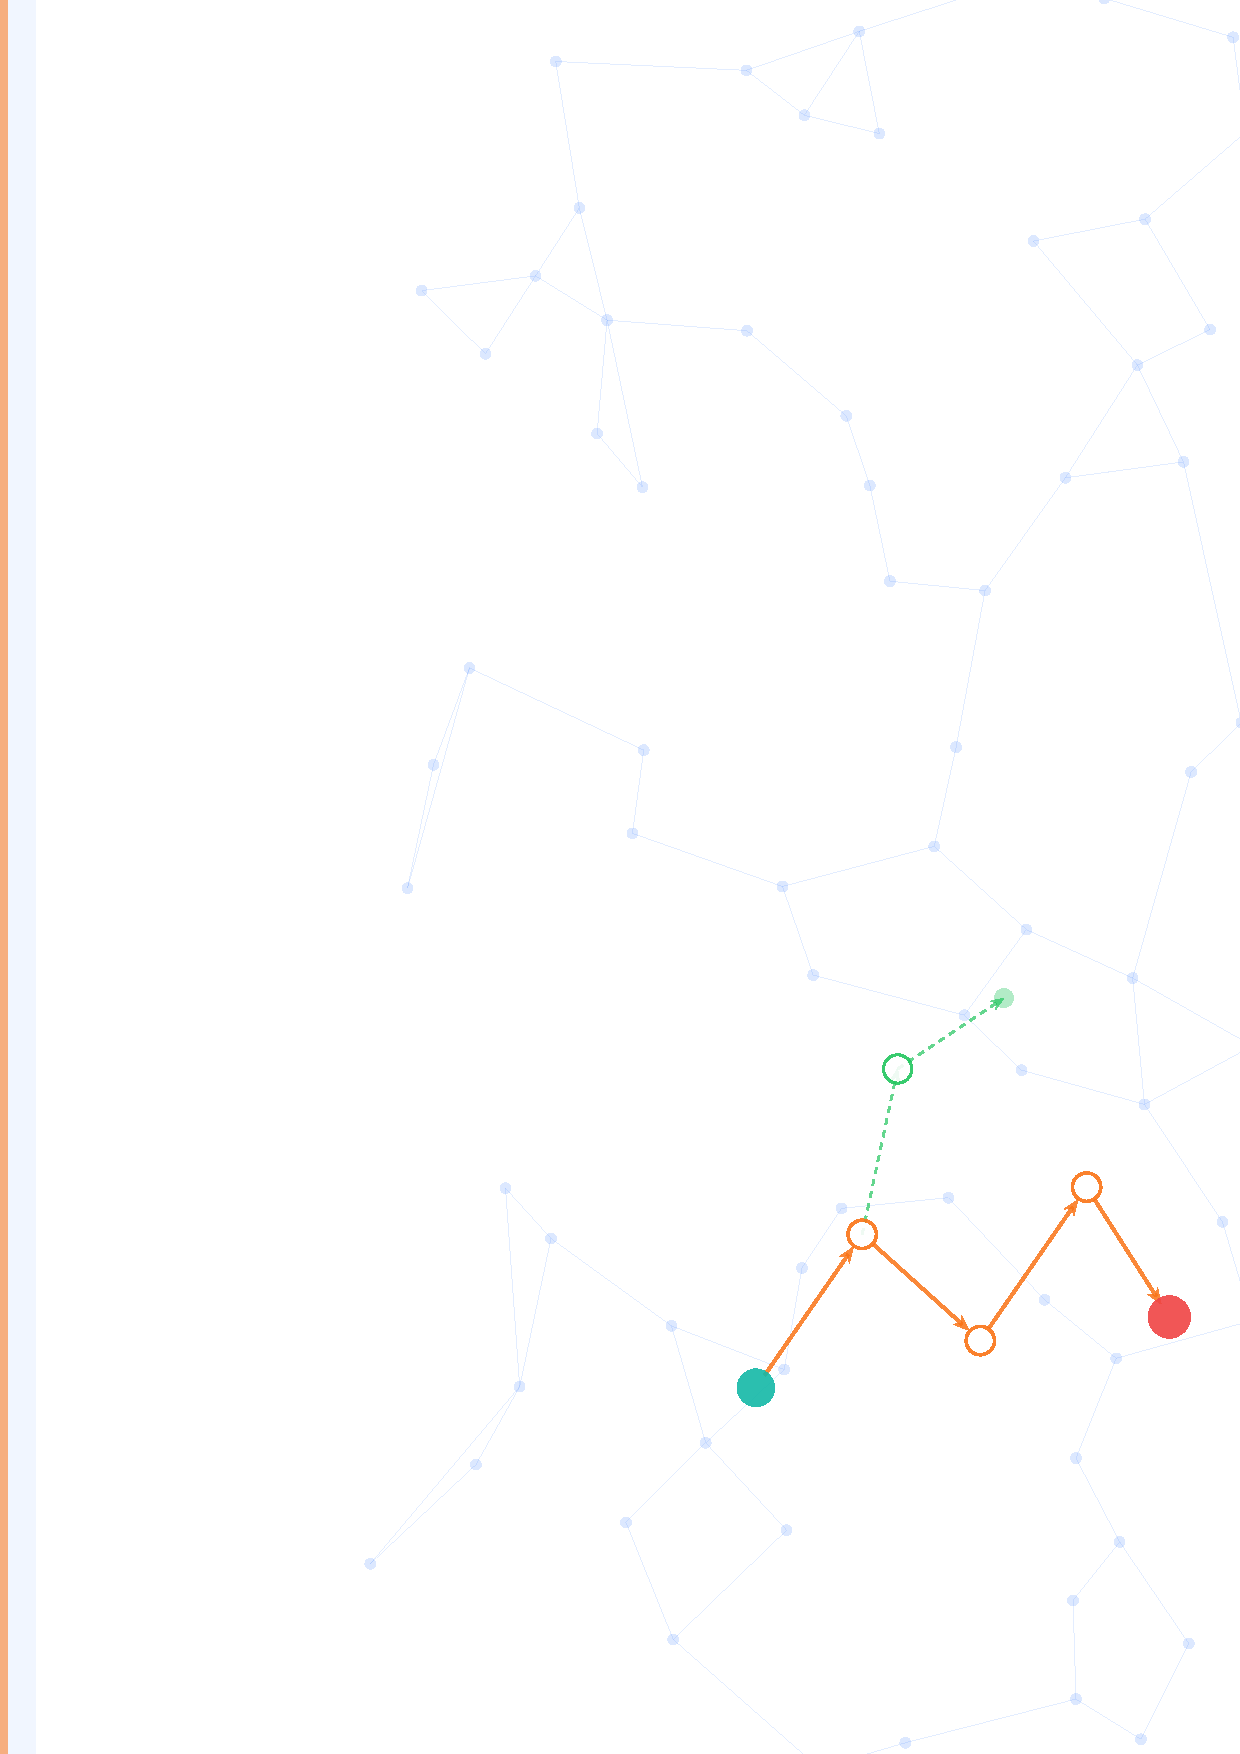
\includegraphics[width=\paperwidth,height=\paperheight]{figuras/portada/portada-fondo}}}

    \frontmatter

    % cuerpo del trabajo: un archivo por capítulo, en el orden de entrega
    \mainmatter
    %!TEX root = ../main.tex
% =============================================================
%  CAPÍTULO 1 — INTRODUCCIÓN            (Entrega 1 · 5 % · 9/6)
% =============================================================

\chapter{Introducción}\label{cap:introduccion}

\begin{guia}[Guía de la cátedra: qué se evalúa en este capítulo]
\begin{enumerate}
    \item \textbf{Descripción del problema}: concreto, anclado en evidencia
          (datos duros con fuente, casos reales, competidores nombrados).
    \item \textbf{Objetivo general}: uno solo, medible, en un párrafo.
          Los \textbf{objetivos específicos} se desprenden de él y
          \emph{no} son los pasos del plan de trabajo.
    \item \textbf{Hipótesis}: explícita, formulada como pregunta o
          afirmación de investigación que pueda responderse en el
          capítulo~\ref{cap:conclusiones}.
    \item \textbf{Relevancia}: por qué importa, a quién beneficia, qué les
          falta a las soluciones existentes.
    \item \textbf{Alcance y recursos}: qué entra y qué no; stack y fuentes
          de datos previstos. El ``alcance que nunca cierra'' es el riesgo
          número uno de la materia.
\end{enumerate}
Extensión orientativa: 4 a 6 páginas. Redacción impersonal, sin ``yo
creo'', oraciones de 15 a 22 palabras, sin palabras vacías
(``claramente'', ``obviamente''). Toda cifra con su fuente citada, por
ejemplo (Autor, año).
\end{guia}

\section{Introducción y contexto}\label{sec:n1.1}

El desarrollo de software moderno exige la incorporación de controles de seguridad en las etapas iniciales del ciclo de vida (enfoque \emph{shift-left}). Tradicionalmente, la auditoría de seguridad se realiza mediante análisis dinámico en fases avanzadas de prueba o a través de analizadores estáticos basados en coincidencia de patrones de texto y firmas de vulnerabilidades conocidas.

La limitación de las herramientas basadas en patrones es que no interpretan la semántica del programa. Tienden a marcar variables como inseguras simplemente por su nombre, o bien pierden el rastro de los datos cuando estos atraviesan varias funciones, desestructuraciones o módulos. Las fallas de seguridad más difíciles de detectar no suelen ser un comando peligroso aislado en una línea, sino un problema de diseño en el modo en que la información viaja entre los componentes del sistema.

Para resolver esto, GraphSAST convierte el código fuente en un grafo dirigido que modela las llamadas, dependencias y mutaciones de las variables. De esta manera, auditar la seguridad se convierte en un problema computable de accesibilidad sobre el grafo.

\section{Definición del problema}\label{sec:n1.2}

Las herramientas SAST convencionales presentan dificultades concretas en proyectos reales:

\paragraph{Falsos positivos por falta de contexto.} Al buscar firmas o patrones de texto, alertan sobre variables que en realidad ya fueron validadas o que no reciben datos externos, y saturan al equipo con reportes que requieren revisión manual.

\paragraph{Pérdida de trazabilidad en flujos complejos.} Cuando una entrada de usuario pasa por middlewares, se asigna a propiedades de objetos o se transfiere entre módulos, los analizadores por expresiones regulares pierden el recorrido del dato.

\paragraph{Dificultad para interpretar reportes planos.} Las listas tradicionales de advertencias muestran la línea del fallo, pero obligan al programador a reconstruir mentalmente todo el camino que siguió la variable desde su origen.

Estas limitaciones definen la pregunta de investigación: ¿puede un analizador basado en grafos de flujo de datos detectar vulnerabilidades de arquitectura con mayor precisión y menor cantidad de falsos positivos que las herramientas basadas en coincidencia de patrones de texto?

\section{Objetivo}\label{sec:n1.3}

\paragraph{Objetivo general:} Desarrollar un sistema de análisis estático de código fuente (SAST) que compile la lógica de una aplicación en un grafo de flujo de datos para auditar, detectar y visualizar de forma interactiva fallas de arquitectura de software y posibles fugas de información, evaluando su precisión sobre proyectos reales.

\paragraph{Objetivos específicos.}

\begin{enumerate}[label=OE-\arabic*.,leftmargin=*]
    \item Construir el analizador sintáctico que procese código fuente TypeScript/JavaScript mediante la biblioteca ts-morph y extraiga los nodos relevantes del Árbol de Sintaxis Abstracta (AST).
    \item Diseñar e implementar el algoritmo de transformación del AST en un grafo dirigido de flujo de datos e invocaciones, con aristas FLOWS\_TO, CALLS, BINDS\_TO, RETURNS y SANITIZED\_BY.
    \item Desarrollar el motor de análisis de taint que detecte caminos source-sink no sanitizados para los patrones CWE-89, CWE-79 y CWE-78, parametrizado mediante un catálogo externo en formato JSON.
    \item Persistir el grafo compilado en la base de datos Neo4j y exponer las consultas de accesibilidad mediante el lenguaje Cypher.
    \item Construir la interfaz web interactiva (TypeScript con Cytoscape.js) que visualice la topología del programa y resalte los recorridos de riesgo detectados.
    \item Validar el prototipo contra un banco de pruebas de casos sintéticos y proyectos reales, midiendo precisión, exhaustividad, falsos positivos y falsos negativos frente a una herramienta de referencia.
\end{enumerate}

\section{Barreras}\label{sec:n1.4}

\begin{itemize}
    \item Complejidad del análisis de lenguajes reales: la construcción de un analizador robusto para un lenguaje moderno implica el tratamiento de numerosas construcciones sintácticas.
    \item Escalabilidad del grafo: el tamaño del grafo crece con el código, por lo que el mantenimiento de tiempos de cómputo razonables constituye un desafío.
    \item Precisión del análisis de taint: la reducción de falsos positivos sin perder vulnerabilidades reales requiere un modelado cuidadoso de fuentes, destinos y sanitizadores.
    \item Alcance del lenguaje: la cobertura de todas las construcciones de un lenguaje resulta inviable en el tiempo del proyecto, por lo que debe acotarse a un subconjunto documentado.
\end{itemize}

\section{Relevancia del proyecto}\label{sec:n1.5}

Las vulnerabilidades de seguridad conllevan un alto costo. Una herramienta capaz de detectar fallas de arquitectura antes de la ejecución, con menor ruido que los analizadores tradicionales y con una visualización comprensible, aporta valor directo a los equipos de desarrollo. En el plano académico, el proyecto integra teoría de grafos, análisis de lenguajes de programación y ciberseguridad aplicada, y produce un artefacto verificable sobre código real.

El trabajo se vincula asimismo con las disciplinas de aseguramiento de la calidad del software (Quality Assurance). Mientras las pruebas funcionales validan el comportamiento dinámico del sistema en ejecución, el análisis estático mediante grafos ofrece un control preventivo sobre el diseño y la arquitectura en una etapa previa a la compilación y el despliegue, lo que sitúa a GraphSAST como complemento del testing tradicional dentro del ciclo de aseguramiento de la calidad.

\section{Hipótesis de investigación}\label{sec:n1.6}

\paragraph{H1.} La representación del código fuente como un grafo de flujo de datos permite identificar vulnerabilidades de arquitectura y recorridos de riesgo con mayor precisión que los analizadores basados en coincidencias aisladas de patrones de texto.

\paragraph{H2.} El análisis de taint estructurado sobre el grafo reduce la tasa de falsos positivos respecto de la detección basada en expresiones regulares.

\paragraph{H3.} La visualización topológica del recorrido del dato facilita la interpretación del riesgo por parte del equipo de desarrollo frente a los listados de errores en texto plano.

\section{Enfoque}\label{sec:n1.7}

El proyecto se enmarca en una investigación aplicada con validación empírica. El prototipo se construye de manera incremental (analizador $\rightarrow$ grafo $\rightarrow$ consultas $\rightarrow$ visualización) y se evalúa cuantitativamente contra un banco de pruebas compuesto por casos sintéticos con fallas conocidas y proyectos reales de código abierto con vulnerabilidades documentadas, midiendo precisión, exhaustividad, falsos positivos, falsos negativos y tiempo de análisis.

\section{Recursos}\label{sec:n1.8}

\begin{itemize}
    \item \textbf{Software: }biblioteca de parsing ts-morph, base de datos de grafos Neo4j, biblioteca de visualización Cytoscape.js, entorno de testing Vitest y control de versiones Git.
    \item \textbf{Datos: }repositorios públicos con vulnerabilidades documentadas y casos sintéticos construidos para la validación.
    \item \textbf{Hardware: }equipo de desarrollo personal.
    \item \textbf{Humanos: }el alumno como responsable del desarrollo y la validación.
\end{itemize}

    \glsresetall % las siglas se vuelven a expandir completas a partir de acá
    %!TEX root = ../main.tex
% =============================================================
%  CAPÍTULO 2 — METODOLOGÍA             (Entrega 2 · 5 % · 5/5)
% =============================================================

\chapter{Metodología y procedimientos}\label{cap:metodologia}

\begin{guia}[Guía de la cátedra: qué se evalúa en este capítulo]
La cátedra exige \textbf{dos metodologías}. El error más común es
entregar solo una.
\begin{enumerate}
    \item \textbf{Metodología de la investigación}: área temática,
          planteamiento y delimitación del problema, marco teórico
          previsto, diseño concreto (fases), indicadores medibles con
          fuente y umbral, técnicas de recolección, instrumentos, datos,
          procesamiento, análisis crítico y síntesis. Tipo de
          investigación: en general, aplicada.
    \item \textbf{Metodología de dirección del proyecto}: marco de trabajo
          justificado, alcance y entregables, cronograma con fechas reales
          (Gantt con hitos que coinciden con las entregas), costos, riesgos
          (referencia al capítulo~\ref{cap:riesgos}), calidad, recursos y
          satisfacción de las partes interesadas.
    \item \textbf{Declaración de uso de IA}: qué tareas fueron asistidas y
          cómo se verificaron. Los prompts se guardan en una carpeta
          compartida con la cátedra.
\end{enumerate}
Extensión orientativa: 6 a 10 páginas. Referencias habituales:
Hernández Sampieri et al. (2014) para investigación y \citet{pmi2021}
para gestión.
\end{guia}

\section{Metodología de la investigación}\label{sec:n2.1}

\subsection{Área temática}\label{sec:n2.1.1}

Ciberseguridad aplicada y análisis de programas: análisis estático de código (SAST), representación del programa mediante grafos y análisis de flujo de datos (taint analysis).

\subsection{Planteamiento del problema}\label{sec:n2.1.2}

¿Puede un analizador basado en grafos de flujo de datos detectar vulnerabilidades de arquitectura con mayor precisión y menos falsos positivos que las herramientas basadas en coincidencia de patrones de texto?

\subsection{Delimitación de la investigación}\label{sec:n2.1.3}

El motor se enfoca en el lenguaje base TypeScript/JavaScript y en tres patrones de riesgo definidos según el catálogo CWE (CWE-89 Inyección SQL, CWE-79 Cross-Site Scripting y CWE-78 Inyección de Comandos). No se incluyen la corrección automática de código ni la integración como complemento (plugin) de entornos de desarrollo comerciales.

\section{Marco teórico}\label{sec:n2.2}

El proyecto se apoya en la teoría de grafos, en los métodos de compilación (análisis sintáctico y árboles de sintaxis abstracta) y en el análisis de flujo de control y de datos. El concepto central es el análisis de taint: el seguimiento de los datos no confiables desde su punto de entrada (source) hasta los puntos críticos donde se utilizan (sink), verificando si fueron sanitizados en el trayecto. Bajo este planteo, la seguridad se formaliza como un problema de accesibilidad sobre un grafo dirigido: existe una vulnerabilidad cuando hay un camino desde un source hasta un sink que no atraviesa un sanitizer.

\section{Diseño concreto de investigación}\label{sec:n2.3}

\subsection{Indicadores}\label{sec:n2.3.1}

\begin{table}[H]
    \centering
    \caption{Indicadores de evaluación del prototipo}
    \label{tab:indicadores}
    \small
    \begin{tabularx}{\textwidth}{l L L}
        \toprule
        \tb{Indicador} & \tb{Definición operativa} & \tb{Medición prevista} \\
        \midrule
        Precisión (Precision) & Proporción de vulnerabilidades reales sobre el total de alertas emitidas. & TP / (TP + FP) \\
        Exhaustividad (Recall) & Proporción de vulnerabilidades reales detectadas sobre el total existente. & TP / (TP + FN) \\
        Falsos positivos (FP) & Alertas generadas sobre código seguro o sanitizado. & Conteo de instancias marcadas erróneamente. \\
        Falsos negativos (FN) & Vulnerabilidades reales presentes que el sistema no detecta. & Conteo de omisiones. \\
        Tiempo de análisis & Tiempo de cómputo para procesar el AST, construir el grafo y ejecutar las consultas por cada 1.000 líneas de código (KLOC). & Medición en segundos mediante scripts de benchmarking. \\
        \bottomrule
    \end{tabularx}
\end{table}

\subsection{Técnicas de recolección de datos}\label{sec:n2.3.2}

Selección de repositorios públicos con vulnerabilidades documentadas y construcción de casos sintéticos con fallas controladas.

\subsection{Instrumentos de recolección de datos}\label{sec:n2.3.3}

Banco de pruebas versionado, scripts de evaluación automatizada y planilla de registro de resultados por caso.

\subsection{Datos}\label{sec:n2.3.4}

Código fuente de los proyectos de prueba, etiquetas de las vulnerabilidades esperadas y mediciones de desempeño del analizador.

\subsection{Procesamiento de los datos}\label{sec:n2.3.5}

Ejecución del analizador sobre cada caso, generación del grafo, ejecución de las consultas de detección y registro de aciertos, falsos positivos y falsos negativos.

\subsection{Análisis de los datos}\label{sec:n2.3.6}

Cálculo de las métricas de desempeño, comparación contra la herramienta de referencia y análisis de los tiempos de cómputo en función del tamaño del código.

\subsection{Síntesis y conclusiones}\label{sec:n2.3.7}

Se evaluarán las hipótesis H1-H3 a partir de los resultados, determinando si el enfoque por grafos mejora la detección y reduce el ruido respecto del análisis por patrones.

\section{Detalle del proyecto}\label{sec:n2.4}

\subsection{Alcance}\label{sec:n2.4.1}

Incluye: motor para el lenguaje base TypeScript/JavaScript, detección de tres patrones de riesgo arquitectónico (CWE-89, CWE-79 y CWE-78), persistencia del grafo, visualización interactiva y banco de pruebas con evaluación reproducible.

No incluye: corrección o refactorización automática del código, ni integración nativa como complemento de entornos de desarrollo comerciales.

\subsection{Tiempos}\label{sec:n2.4.2}

El cronograma se organiza en etapas de desarrollo, validación y redacción, ajustables al calendario académico.

\begin{table}[H]
    \centering
    \caption{Cronograma de desarrollo e implementación}
    \label{tab:hitos}
    \small
    \begin{tabularx}{\textwidth}{l L l}
        \toprule
        \tb{Etapa / Hito} & \tb{Entregable} & \tb{Período estimado} \\
        \midrule
        Hito 1 & Analizador y extracción del Árbol de Sintaxis Abstracta (AST). & Mes 1-2 \\
        Hito 2 & Algoritmo de construcción del grafo de flujo de datos. & Mes 3-4 \\
        Hito 3 & Motor de consultas (taint analysis) e integración con la base de datos de grafos. & Mes 5-6 \\
        Hito 4 & Interfaz web interactiva de visualización. & Mes 7-8 \\
        Hito 5 & Validación con proyectos reales, benchmarking y redacción de la memoria final. & Mes 9-10 \\
        \bottomrule
    \end{tabularx}
\end{table}

\subsection{Costos}\label{sec:n2.4.3}

El proyecto se plantea como un prototipo académico de bajo costo, priorizando herramientas libres, documentación pública y recursos propios.

\begin{table}[H]
    \centering
    \caption{Costos estimados del proyecto}
    \label{tab:costos}
    \small
    \begin{tabularx}{\textwidth}{l L L}
        \toprule
        \tb{Recurso} & \tb{Tipo} & \tb{Costo estimado} \\
        \midrule
        Hardware & Equipo de cómputo personal de desarrollo. & Sin costo adicional \\
        Software y base de datos & ts-morph, Neo4j Community, Cytoscape.js, Vite, Vitest. & Licencias open source / gratuitas \\
        Datos de prueba & Repositorios públicos (OWASP, NIST SARD, GitHub). & Acceso público sin costo \\
        Total estimado & — & USD 0,00 \\
        \bottomrule
    \end{tabularx}
\end{table}

\subsection{Riesgos}\label{sec:n2.4.4}

\begin{table}[H]
    \centering
    \caption{Riesgos principales y mitigación}
    \label{tab:riesgos-iniciales}
    \small
    \begin{tabularx}{\textwidth}{L l l L}
        \toprule
        \tb{Riesgo} & \tb{Probabilidad} & \tb{Impacto} & \tb{Mitigación} \\
        \midrule
        Complejidad excesiva en el análisis del lenguaje & Media & Alto & Emplear bibliotecas de parsing maduras y acotar las construcciones sintácticas soportadas a un subconjunto documentado. \\
        Degradación del rendimiento al escalar el grafo & Media & Medio & Optimizar los índices en la base de datos, acotar la profundidad de búsqueda en los recorridos y limitar el análisis de dependencias externas. \\
        Generación elevada de falsos positivos & Media & Alto & Refinar la definición de sources, sinks y sanitizadores en el catálogo, e incorporar verificaciones de contexto en el motor de consultas. \\
        \bottomrule
    \end{tabularx}
\end{table}

\subsection{Calidad}\label{sec:n2.4.5}

La calidad se asegura mediante un banco de pruebas versionado, una evaluación automatizada y reproducible, y pruebas unitarias del software (Vitest) por módulo.

\subsection{Recursos}\label{sec:n2.4.6}

Humanos: el alumno. Tecnológicos: biblioteca de parsing (ts-morph), base de datos de grafos (Neo4j), biblioteca de visualización (Cytoscape.js) y entorno de testing (Vitest). Materiales: equipo de desarrollo personal.

\subsection{Satisfacción}\label{sec:n2.4.7}

El grado de satisfacción se mide por la precisión alcanzada y la reducción de falsos positivos respecto de la herramienta de referencia, y por la claridad de la visualización para identificar el recorrido del riesgo.

    %!TEX root = ../main.tex
% =============================================================
%  CAPÍTULO 3 — MARCO TEÓRICO Y ESTADO DEL ARTE
%                                       (Entrega 3 · 10 % · 28/7)
% =============================================================

\chapter{Síntesis de la literatura consultada}\label{cap:marco-teorico}

\begin{guia}[Guía de la cátedra: qué se evalúa en este capítulo]
\begin{enumerate}
    \item \textbf{Estado del arte}: investigaciones nacionales,
          internacionales y productos similares, por separado. De cada
          trabajo: qué hizo y qué resultados obtuvo, con métricas.
    \item \textbf{Brechas identificadas}: qué falta en lo existente y
          justifica \emph{este} proyecto. Es lo que separa un estado del
          arte de un listado. Incluir también los resultados negativos de
          la literatura.
    \item \textbf{Bases teóricas}: desarrollan las variables del título y su
          relación. Cada concepto termina explicando cómo se usa en el
          proyecto (teoría instrumental, no de relleno). Citas canónicas
          antes que tutoriales.
    \item \textbf{Marco conceptual}: conceptos que se nombran pero no se
          desarrollan. Los términos del glosario se marcan con
          \verb|\gls{}|, por ejemplo \gls{g:mvp} y \gls{prototipo}.
    \item \textbf{Calidad bibliográfica}: papers, tesis y libros de
          editoriales serias, con datos completos. Wikipedia y blogs restan.
    \item \textbf{Entrevistas a especialistas} (si las hay): fecha, nombre,
          cargo y aporte; transcripción en el apéndice~\ref{apx:entrevista}.
\end{enumerate}
Errores que la cátedra marca: falta de coherencia interna, bibliografía
superficial, información irrelevante o redundante. Es uno de los
capítulos más extensos (orientativo: 20 a 30 páginas).
\end{guia}

\section{Estado del Arte}\label{sec:n3.1}

\subsection{Investigación Nacional}\label{sec:n3.1.1}

En el ámbito académico nacional existen antecedentes directos en análisis estático de programas y, en particular, en análisis de contaminación (taint analysis) aplicado a JavaScript. La producción más relevante proviene del Departamento de Computación de la Facultad de Ciencias Exactas y Naturales de la Universidad de Buenos Aires (FCEyN-UBA) y del Instituto de Investigación en Ciencias de la Computación (ICC, UBA-CONICET), cuyas líneas de investigación se orientan al análisis automático de programas para su comprensión, verificación y validación.

Dentro de esa línea de trabajo, \citet{balbi2023} desarrolla una investigación centrada en la inferencia automática de especificaciones de taint analysis para el lenguaje JavaScript. El trabajo parte de la premisa de que la efectividad del análisis de contaminación no depende únicamente del motor de rastreo, sino de la calidad de las especificaciones que definen qué elementos del programa constituyen puntos de entrada (sources) o de riesgo (sinks). La solución propuesta combina un método basado en aprendizaje automático con el motor de análisis estático CodeQL, empleado como infraestructura de consulta subyacente.

Esta investigación se articula con producción científica de proyección internacional. \citet{dutta2022} presentan InspectJS en el 44th International Conference on Software Engineering (ICSE-SEIP), trabajo que aborda la inferencia de especificaciones de taint para JavaScript mediante similitud de código y retroalimentación del usuario. Los autores sostienen que el mecanismo de rastreo de contaminación se implementa una única vez en el motor y luego se parametriza con distintos conjuntos de sources, sinks y sanitizers, lo que permite detectar categorías diversas de vulnerabilidades sin modificar la lógica interna del analizador. Este principio de desacoplamiento entre el motor de análisis y el catálogo de reglas constituye un fundamento directo del diseño de catálogo externo en formato JSON adoptado en el presente proyecto.

En el plano de la investigación aplicada, se registran trabajos nacionales que emplean el análisis estático como instrumento de auditoría sobre productos concretos. La Universidad Argentina de la Empresa (UADE) desarrolló una investigación orientada a evaluar las características de seguridad de videojuegos basados en NFT Gaming (2021-2022), combinando el análisis estático del código fuente en busca de vulnerabilidades con el análisis dinámico de los datos recopilados por las aplicaciones \citep{villan2022}.

Como ámbito de difusión científica, el Simposio Argentino de Ingeniería de Software (ASSE), integrado a las Jornadas Argentinas de Informática (JAIIO) organizadas por la Sociedad Argentina de Informática e Investigación Operativa (SADIO) desde 1961, constituye el foro nacional de referencia para la producción en ingeniería de software y ha sido consultado como fuente de antecedentes locales.

\subsection{Brechas Identificadas en la Investigación Nacional}\label{sec:n3.1.2}

El relevamiento de la literatura nacional permite delimitar con precisión el aporte del presente proyecto:

\paragraph{Dependencia de motores industriales preexistentes:} los antecedentes nacionales de investigación fundamental operan sobre infraestructuras de análisis ya construidas (particularmente CodeQL) y concentran su innovación en la capa de inferencia de especificaciones. La construcción propia del recorrido posterior al análisis sintáctico —la transformación del árbol en grafo de flujo de datos, su persistencia y el motor de consultas autónomo— permanece fuera del alcance de estos trabajos, que la asumen como un componente disponible.

\paragraph{Ausencia de implementaciones académicas reproducibles de extremo a extremo:} no se identifican en el ámbito nacional desarrollos académicos de código abierto que documenten e implementen de manera integral la compilación directa del código fuente a un grafo de propiedades persistido, junto con el motor de consultas de accesibilidad y un banco de pruebas reproducible por terceros.

\paragraph{Orientación aplicada desacoplada del diseño del analizador:} los trabajos de investigación aplicada locales emplean herramientas comerciales o de código abierto existentes como instrumentos de auditoría sobre software final, sin abordar el diseño algorítmico del motor de detección ni la evaluación cuantitativa de su precisión frente a enfoques alternativos.

\paragraph{Escasa exploración de la visualización topológica del riesgo:} la representación interactiva del recorrido del dato contaminado sobre la topología del programa, orientada a reducir el esfuerzo de interpretación del hallazgo por parte del equipo de desarrollo, no aparece tratada como objeto de estudio en los antecedentes nacionales relevados.

\subsection{Investigaciones Internacionales}\label{sec:n3.1.3}

A nivel internacional, la representación del código mediante grafos y el análisis de flujo de datos cuentan con antecedentes teóricos y empíricos fundamentales:

\paragraph{Code Property Graphs (CPG):} \citet{yamaguchi2014} formalizaron la representación unificada del código fuente combinando en una misma estructura de grafo el Árbol de Sintaxis Abstracta (AST), el Grafo de Flujo de Control (CFG) y el Grafo de Dependencia de Datos (DDG). Este trabajo mostró que la detección de vulnerabilidades puede expresarse como un problema de consulta de accesibilidad sobre grafos.

\paragraph{Object Dependence Graphs (ODG):} \citet{li2022} desarrollaron un modelo basado en grafos de dependencia de objetos para detectar vulnerabilidades en el ecosistema Node.js / JavaScript, demostrando que el rastreo de objetos en lenguajes dinámicos permite abordar patrones de riesgo no detectados por el análisis estático convencional.

\paragraph{Estudios comparativos de herramientas SAST en Node.js:} \citet{brito2023} evaluaron empíricamente la efectividad de herramientas de análisis estático sobre paquetes reales del ecosistema Node.js, caracterizando sus limitaciones de cobertura y precisión.

\subsection{Productos Similares}\label{sec:n3.1.4}

En la industria del software existen herramientas consolidadas que aplican principios de análisis de flujo de datos e inspección de código:

\begin{table}[H]
    \centering
    \caption{Comparación de herramientas SAST similares}
    \label{tab:comparativa}
    \small
    \begin{tabularx}{\textwidth}{l L L L}
        \toprule
        \tb{Herramienta} & \tb{Motor de Análisis} & \tb{Alcance y Enfoque} & \tb{Diferenciación con GraphSAST} \\
        \midrule
        CodeQL (GitHub / Semmle) & Motor relacional basado en grafos interpretados con lenguaje declarativo QL. & Plataforma profesional multilenguaje de alcance industrial. & Requiere infraestructura y compilación pesada; GraphSAST implementa un motor liviano enfocado en TypeScript/JavaScript con persistencia nativa en base de datos de grafos y visualización web interactiva. \\
        Semgrep & Motor de coincidencia de patrones sintácticos abstractos con soporte de taint mode. & Análisis rápido en pipelines de CI/CD basado en reglas declarativas en YAML. & Su enfoque principal es la ejecución de reglas en línea de comandos; no persiste la topología completa del programa en una base de datos de grafos para consultas de arquitectura. \\
        Joern & Plataforma de código abierto basada en Code Property Graphs (CPG). & Análisis estático avanzado enfocado en C/C++ y Java utilizando la base OverflowDB. & Orientado a análisis por consola mediante entorno REPL (Scala); GraphSAST simplifica la inspección mediante un panel web con renderizado dinámico de nodos. \\
        \bottomrule
    \end{tabularx}
\end{table}

\section{Marco Teórico}\label{sec:n3.2}

En consonancia con la metodología académica establecida, se definen en primer lugar las variables de investigación y su relación teórica:

\paragraph{Variable independiente ($V_1$).} representación del código fuente mediante grafos de flujo de datos (Data Flow Graphs).

\paragraph{Variable dependiente ($V_2$).} detección estática de vulnerabilidades de arquitectura de software y precisión en el análisis de contaminación (Taint Analysis).

\paragraph{Relación entre las Variables:} la hipótesis central de este trabajo sostiene que transformar la estructura sintáctica del código fuente en una representación matemática en forma de grafo dirigido permite formular la detección de vulnerabilidades como un problema formal de accesibilidad (reachability), mejorando la precisión y reduciendo la tasa de falsos positivos en comparación con los analizadores estáticos basados en coincidencia de patrones de texto.

\subsection{Análisis Estático de Código Fuente (SAST) y \enquote{Building Security In}}\label{sec:n3.2.1}

El análisis estático de código fuente consiste en la evaluación del código de una aplicación sin requerir su ejecución dinámica \citep{nielson1999}. En la ingeniería de software, \citet{mcgraw2006} formalizó el principio de incorporar prácticas de seguridad de manera intrínseca desde las fases iniciales del ciclo de vida del desarrollo de software (SDLC), enfoque que la industria denominaría posteriormente bajo el término Shift-Left Security. Detectar y corregir defectos de diseño y vulnerabilidades durante la fase de codificación evita que la deuda técnica de seguridad se propague hacia los entornos de prueba o producción, reduciendo los costos de remediación.

\subsection{Compiladores, Análisis Léxico, Parsing y Árboles de Sintaxis Abstracta (AST)}\label{sec:n3.2.2}

La teoría clásica de compiladores establece que el procesamiento del código fuente comienza con la fase de análisis léxico (scanning), donde la secuencia lineal de caracteres se convierte en una serie de tokens, seguida por el análisis sintáctico (parsing), que construye una representación jerárquica denominada Árbol de Sintaxis Abstracta (Abstract Syntax Tree - AST) \citep{aho2006}. El AST representa la estructura gramatical del programa en forma de árbol.

En el marco de este proyecto, el proceso de parsing se fundamenta en la API del compilador oficial de TypeScript a través de la biblioteca ts-morph. Esta herramienta permite consumir código fuente escrito en JavaScript/TypeScript y extraer una representación estructurada compuesta por nodos sintácticos (tales como declaraciones de funciones, asignaciones de variables, llamadas a métodos e identificadores).

\subsection{Representación del Código mediante Grafos: Call Graph y Data Flow Graph (DFG)}\label{sec:n3.2.3}

Aunque el AST proporciona la estructura sintáctica del programa, no modela de forma explícita las relaciones de dependencia ni el recorrido de los datos a través de las diferentes funciones y módulos \citep{yamaguchi2014}. Para superar esta limitación, la literatura propone construir dos representaciones sobre el AST:

\paragraph{Call Graph (Grafo de Invocaciones):} grafo dirigido donde los nodos corresponden a funciones o métodos y las aristas dirigidas representan llamadas efectivas entre ellos, permitiendo realizar un análisis tanto intraprocedural (dentro de una misma función) como interprocedural (entre distintos archivos y módulos).

\paragraph{Data Flow Graph - DFG (Grafo de Flujo de Datos):} grafo dirigido $G = (V, E)$ donde el conjunto de vértices $V$ representa variables, operaciones e identificadores, y el conjunto de aristas dirigidas $E$ modela la propagación y mutación de los valores.

En la fundamentación de este trabajo, el Grafo de Flujo de Datos formaliza las relaciones entre nodos mediante los siguientes tipos de aristas dirigidas:

\begin{itemize}
    \item \textbf{FLOWS\_TO:} indica la transferencia o asignación directa del valor de una variable a otra.
    \item \textbf{CALLS:} representa la invocación de una función o método con paso de parámetros.
    \item \textbf{BINDS\_TO:} modela la vinculación semántica entre parámetros formales y argumentos reales.
    \item \textbf{RETURNS:} representa el retorno de un valor desde el ámbito de una función hacia el contexto invocador.
    \item \textbf{SANITIZED\_BY:} modela la intercepción y neutralización del dato por parte de una función de validación o limpieza.
\end{itemize}

\begin{figure}[H]
    \centering
    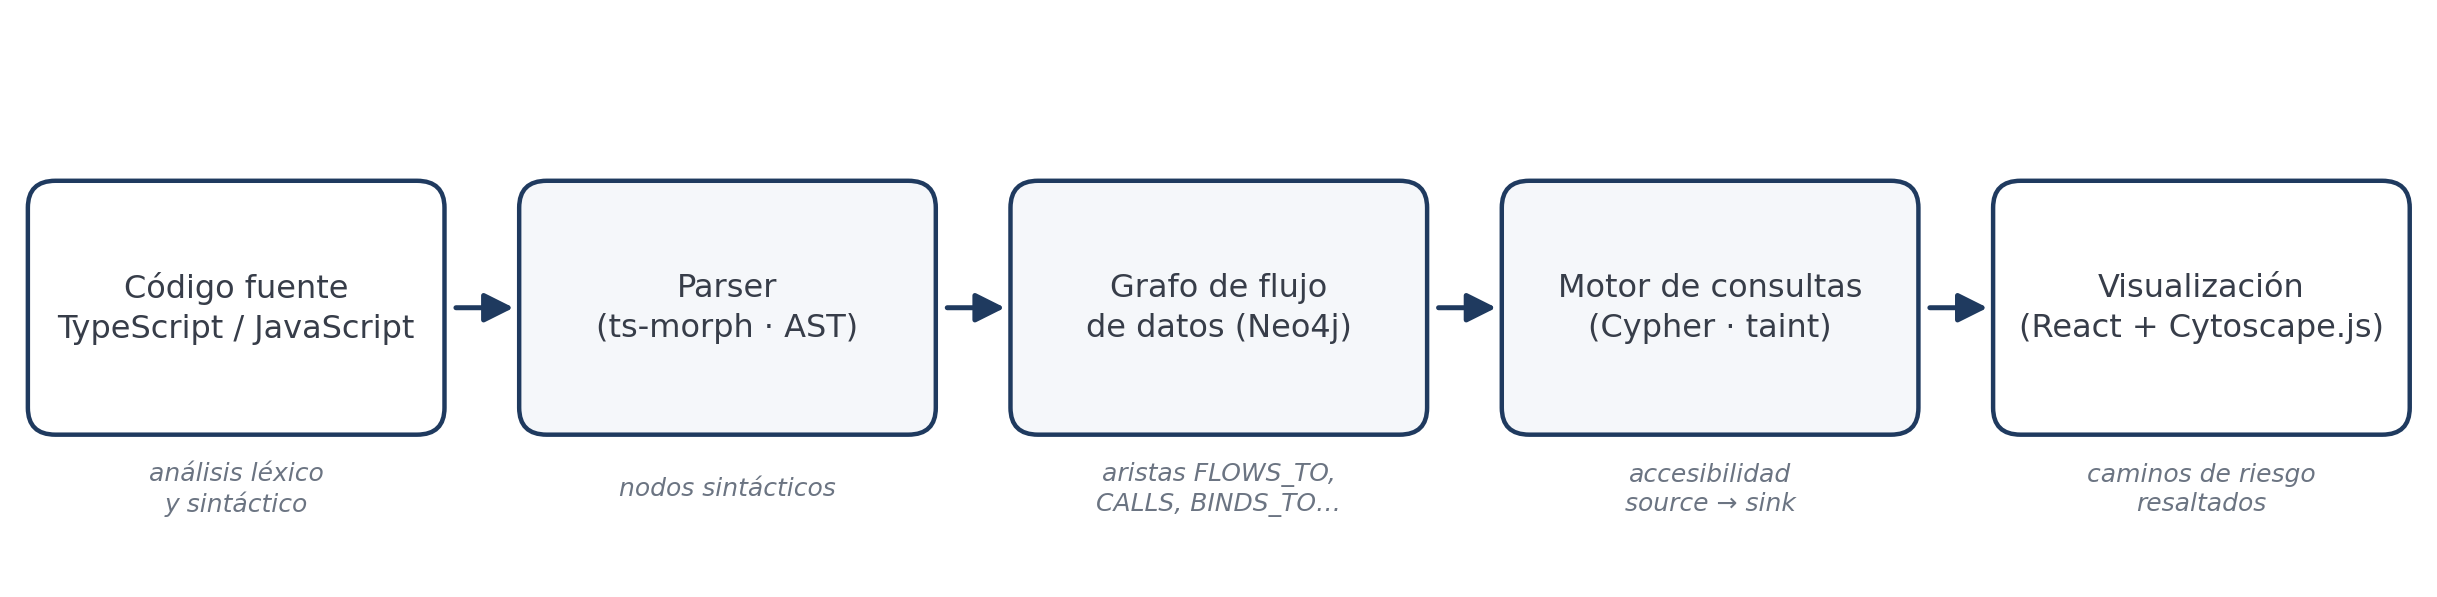
\includegraphics[width=\textwidth]{figuras/flujo-general.png}
    \caption{Flujo general de procesamiento de GraphSAST: código fuente, parser, grafo de flujo de datos, consultas y visualización}
    \label{fig:flujo-general}
\end{figure}

\subsection{Análisis de Contaminación (Taint Analysis)}\label{sec:n3.2.4}

El análisis de contaminación (taint analysis) es un método formal fundamentado en la teoría del flujo de información \citep{denning1976,sabelfeld2003,nielson1999} para verificar si datos provenientes de fuentes no confiables pueden alcanzar operaciones sensibles sin una sanitización intermedia adecuada. El modelo teórico se define mediante la tupla $(S, K, F)$:

\paragraph{Source ($S$, origen).} conjunto de nodos que representan puntos de entrada de información externa al programa no controlada por el sistema (por ejemplo, parámetros HTTP req.body, req.query, o entradas de usuario).

\paragraph{Sink ($K$, destino).} conjunto de nodos que representan operaciones o funciones críticas donde la utilización de un dato no seguro genera una vulnerabilidad (por ejemplo, consultas SQL db.query(), ejecución de comandos child\_process.exec(), o renderizado en interfaz).

\paragraph{Sanitizer ($F$, sanitizador).} conjunto de nodos u operaciones que aplican filtros, codificaciones o validaciones que remueven la condición de contaminación del dato.

Desde la perspectiva de la teoría de grafos, una vulnerabilidad de seguridad se define formalmente como un problema de accesibilidad (reachability): existe una vulnerabilidad si y solo si en el grafo $G$ existe un camino dirigido $p = (v_1, v_2, \ldots, v_n)$ tal que $v_1 \in S$, $v_n \in K$ y $\forall v_i \in p,\ v_i \notin F$.

\begin{figure}[H]
    \centering
    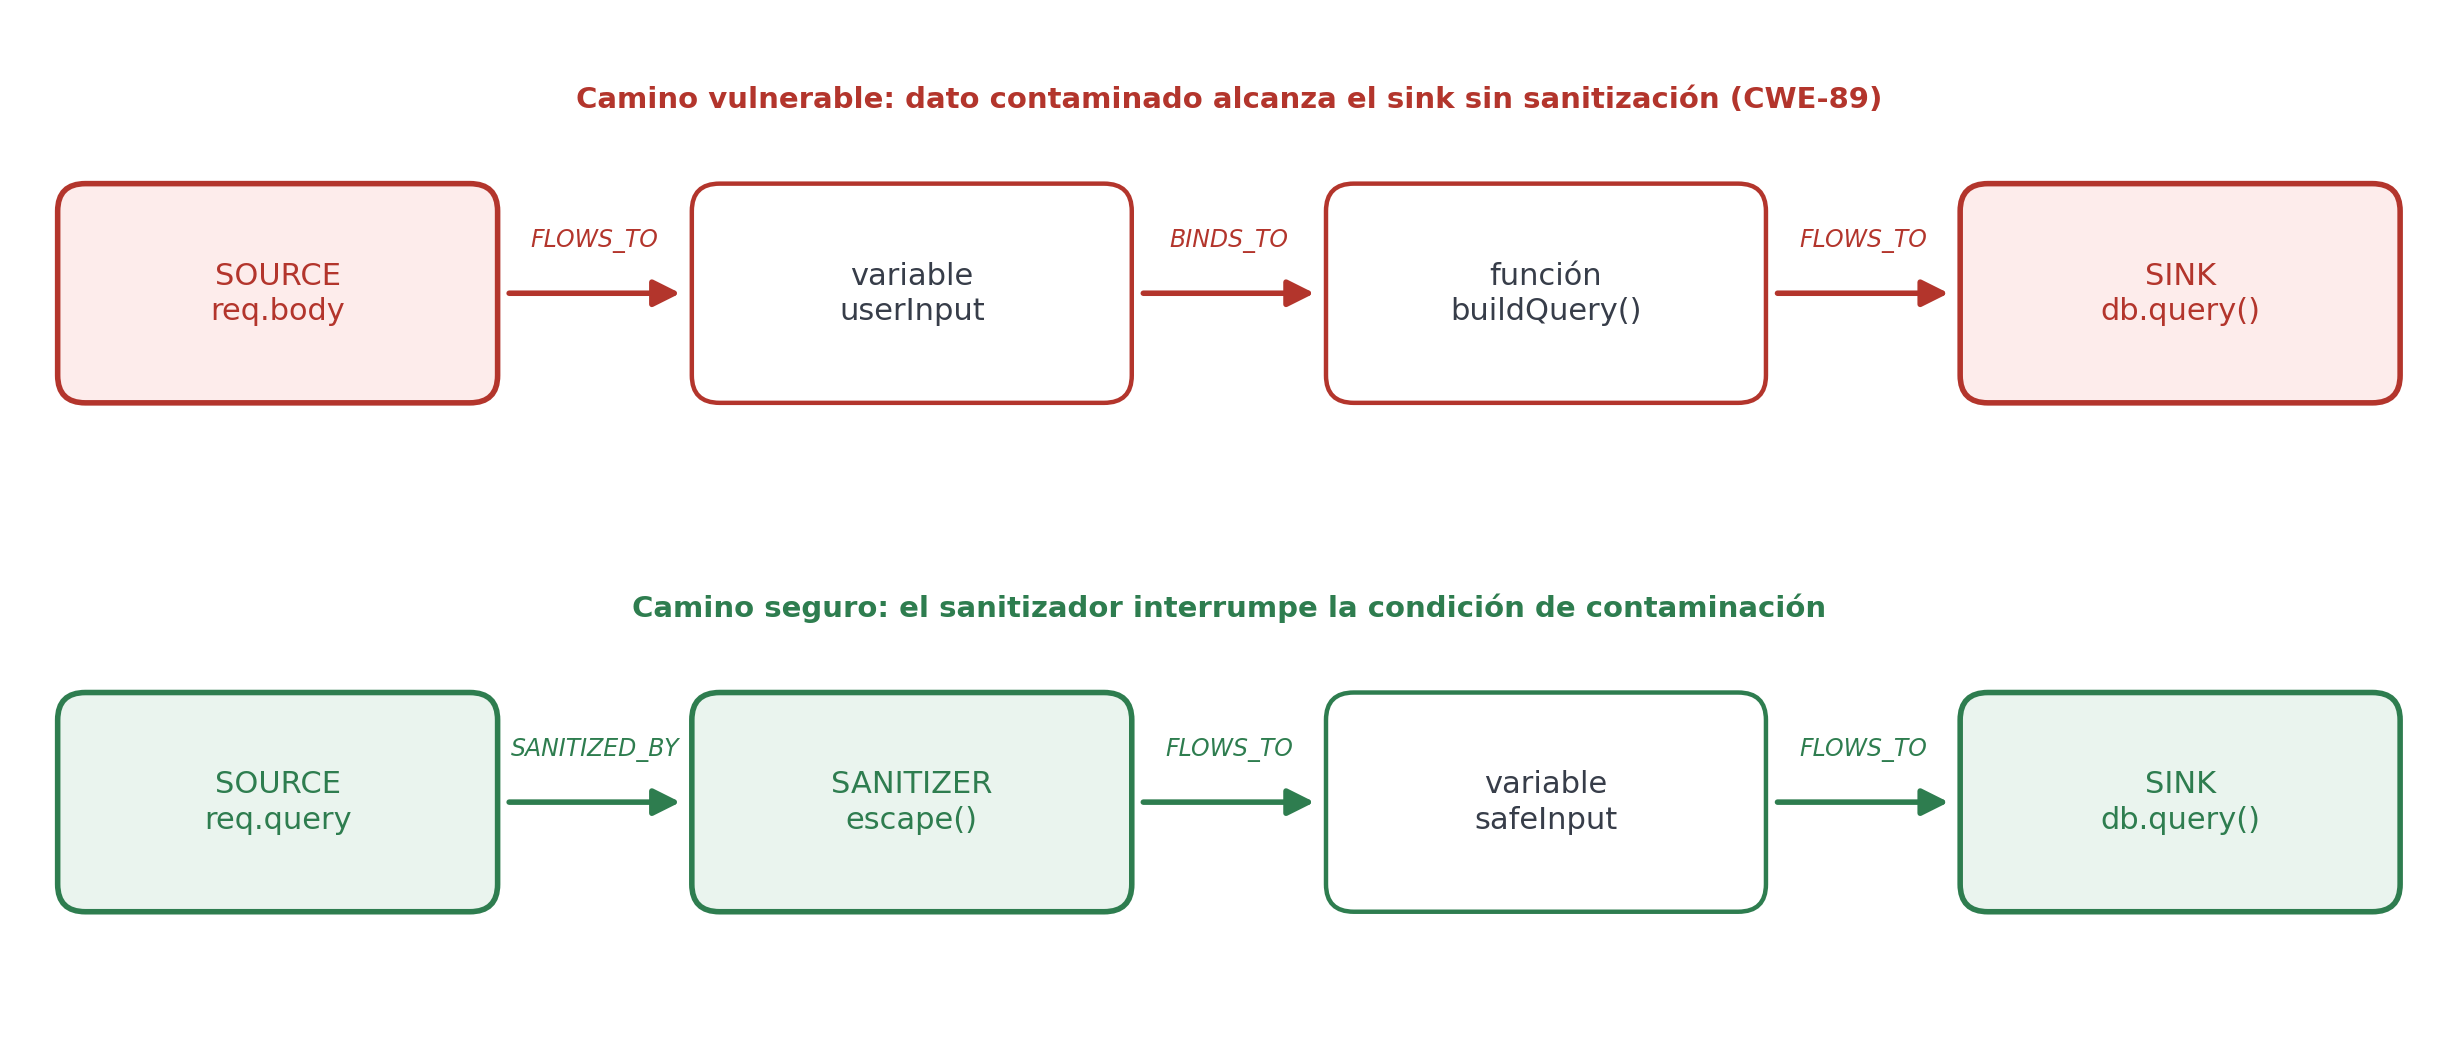
\includegraphics[width=0.9\textwidth]{figuras/source-sink.png}
    \caption{Recorrido source-sink utilizado en el análisis de taint}
    \label{fig:source-sink}
\end{figure}

\subsection{Bases de Datos Orientadas a Grafos y Motor de Consultas (Neo4j y Cypher)}\label{sec:n3.2.5}

Una base de datos orientada a grafos es un sistema de gestión de bases de datos diseñado para almacenar y consultar estructuras de red compuestas por nodos, aristas y propiedades \citep{robinson2013}. Su ventaja técnica fundamental frente a las bases de datos relacionales en la ejecución de recorridos locales reside en la propiedad de adyacencia sin índices (index-free adjacency), donde cada nodo mantiene referencias directas hacia sus nodos vecinos, permitiendo explorar caminos sin realizar operaciones costosas de cruce (joins).

Para la aplicación en este proyecto, se adopta Neo4j como motor de persistencia del grafo compilado y el lenguaje Cypher como motor de consultas declarativo. Cypher permite expresar patrones de accesibilidad de longitud variable entre nodos de tipo Source y Sink, recorriendo de forma combinada las relaciones de flujo de datos, invocación, vinculación de parámetros y retorno, y descartando aquellos caminos en los que interviene una operación de sanitización.

\subsection{Catálogo de Vulnerabilidades de Arquitectura (CWE)}\label{sec:n3.2.6}

La clasificación de vulnerabilidades se fundamenta en el estándar internacional Common Weakness Enumeration (CWE) de la organización MITRE \citep{mitrecwe}. En este trabajo, el motor de detección se enfoca en tres patrones de riesgo arquitectónico:

\paragraph{CWE-89 (SQL Injection):} ocurre cuando datos no sanitizados de una source fluyen hacia la construcción de consultas SQL dinámicas en un sink de base de datos.

\paragraph{CWE-79 (Cross-Site Scripting - XSS):} ocurre cuando datos no confiables alcanzan salidas del navegador o respuestas HTTP sin la debida codificación.

\paragraph{CWE-78 (Command Injection):} ocurre cuando entradas externas fluyen hacia funciones de ejecución de comandos del sistema operativo (exec, spawn).

\subsection{Visualización de Software e Interfaz Interactiva de Grafos}\label{sec:n3.2.7}

La disciplina de visualización de software (Software Visualization) sostiene que la representación gráfica interactiva de las estructuras y flujos internos del programa reduce la carga cognitiva en la comprensión de la arquitectura y la identificación de fallas \citep{diehl2007}. La integración de herramientas de renderizado de grafos como Cytoscape.js en entornos web modernos permite transformar los hallazgos de seguridad en diagramas interactivos donde los caminos críticos Source $\rightarrow$ Sink se resaltan sobre la topología del código, facilitando el diagnóstico por parte del desarrollador.

\section{Marco Conceptual}\label{sec:n3.3}

\subsection{Vulnerabilidad de Arquitectura}\label{sec:n3.3.1}

Defecto de seguridad cuya existencia no se manifiesta en una sentencia aislada del código, sino en la forma en que los componentes del sistema se vinculan entre sí y en el recorrido que la información describe a través de ellos. A diferencia de las vulnerabilidades localizadas —identificables mediante la inspección de una única línea o expresión—, una vulnerabilidad de arquitectura requiere reconstruir la propagación del dato a través de múltiples funciones, módulos o capas de abstracción para poder ser detectada. Su identificación exige, en consecuencia, una representación del programa que exceda el ámbito de la sentencia individual.

\subsection{Deuda Técnica de Seguridad}\label{sec:n3.3.2}

Especialización del concepto de deuda técnica que cuantifica el costo diferido y el riesgo acumulado en un sistema de software debido a decisiones de diseño o deficiencias de seguridad no resueltas en el código fuente. Una alta deuda técnica de seguridad incrementa la superficie de ataque del sistema.

\subsection{Indicadores de Calidad del Analizador: Precisión, Exhaustividad, Falsos Positivos y Negativos}\label{sec:n3.3.3}

Conjunto de métricas estadísticas utilizadas para medir el desempeño de un sistema SAST:

\paragraph{Falso positivo (FP).} alerta reportada por el analizador sobre un fragmento de código que en realidad es seguro o está correctamente sanitizado.

\paragraph{Falso negativo (FN).} vulnerabilidad real presente en el código fuente que el analizador omite detectar.

\paragraph{Precisión (Precision):} proporción de vulnerabilidades reales detectadas sobre el total de alertas emitidas por la herramienta:

\[ \mathit{Precision} = \frac{TP}{TP + FP} \]

\paragraph{Exhaustividad (Recall):} proporción de vulnerabilidades reales detectadas sobre el total de vulnerabilidades existentes en el programa:

\[ \mathit{Recall} = \frac{TP}{TP + FN} \]

\subsection{Accesibilidad (Reachability) en Grafos Dirigidos}\label{sec:n3.3.4}

Propiedad matemática de la teoría de grafos que determina si existe una secuencia de aristas dirigidas que conecte un nodo de origen $u$ con un nodo de destino $v$. En el contexto del análisis estático, se utiliza para verificar formalmente si existe flujo de información entre dos puntos del programa.

\subsection[Sensibilidad en el Análisis de Programas]{Sensibilidad en el Análisis de Programas\newline (Flow-, Context- y Path-Sensitivity)}\label{sec:n3.3.5}

Clasificación teórica que define el grado de precisión y el nivel de abstracción adoptado por un algoritmo de análisis estático \citep{nielson1999}:

\paragraph{Sensibilidad al Flujo (Flow-sensitivity):} un análisis es sensible al flujo si tiene en cuenta el orden de ejecución de las sentencias del programa. Un análisis insensible al flujo considera las sentencias como un conjunto no ordenado.

\paragraph{Sensibilidad al Contexto (Context-sensitivity):} un análisis es sensible al contexto si distingue entre las diferentes invocaciones de una misma función según la pila de llamadas (call stack) desde donde fue emitida, evitando mezclar los flujos de datos de distintas llamadas.

\paragraph{Sensibilidad al Camino (Path-sensitivity):} un análisis es sensible al camino si evalúa la validez de los predicados o condiciones lógicas de las ramificaciones (if, switch), diferenciando rutas de ejecución factibles de aquellas que son inalcanzables.

    %!TEX root = ../main.tex
% =============================================================
%  CAPÍTULO 4 — MARCO TECNOLÓGICO       (Entrega 4 · 10 % · 25/8)
% =============================================================

\chapter{Marco tecnológico}\label{cap:marco-tecnologico}

\begin{guia}[Guía de la cátedra: qué se evalúa en este capítulo]
Documenta el \emph{cómo}. No es un manual de uso: es la justificación
de cada elección tecnológica. Regla: nada ``porque sí''.
\begin{enumerate}
    \item \textbf{Arquitectura}: diagrama con componentes y conexiones,
          responsabilidad y tecnología de cada uno, flujo de datos y
          justificación del estilo arquitectónico con alternativas
          evaluadas (Sommerville, 2016).
    \item \textbf{Prototipo o \gls{g:mvp}}: cuál es y por qué; alcance
          implementado vs.\ simulado; capturas o enlace; cómo se probó.
    \item \textbf{Stack}: por tecnología, nombre, versión, capa, por qué
          (madurez, comunidad, costo, conocimiento del equipo) y qué
          alternativas se descartaron.
    \item \textbf{Infraestructura y base de datos}: dónde se aloja cada
          componente, escalabilidad, costos (enlazados al
          capítulo~\ref{cap:economica}), motor y modelo de datos.
    \item \textbf{Diseño y \gls{ux}}: quién lo usa, mockups, decisiones de
          diseño y \textbf{cómo se validó con usuarios} (la cátedra lo marca
          como importante; cuestionario en el apéndice~\ref{apx:encuesta}).
    \item \textbf{Seguridad, calidad y despliegue}: autenticación, control
          de acceso, cifrado, plan de pruebas, repositorio, \gls{cicd} y
          monitoreo.
\end{enumerate}
\end{guia}

\section{Arquitectura del sistema}\label{sec:n4.1}

El sistema se diseñó como un pipeline por etapas sucesivas y desacopladas. Esta estructura modular permite que cada componente cumpla un rol único dentro del procesamiento: el análisis sintáctico genera el AST, los constructores crean los nodos y aristas de la representación intermedia, y el motor de taint opera sobre el grafo final. La división simplifica además la estrategia de pruebas, ya que permite aislar y validar cada fase mediante pruebas unitarias independientes sin necesidad de ejecutar el pipeline completo para verificar un módulo interno.

La decisión se refleja además en la estrategia de pruebas. Al ejecutar la suite de tests, cada etapa se valida de forma independiente, lo que permite identificar con precisión en qué componente del pipeline se produce una falla. Una arquitectura monolítica impediría este nivel de aislamiento, dado que mezclaría el análisis sintáctico con el análisis semántico y forzaría a probar el sistema como una unidad indivisible.

\subsection{Organización en paquetes}\label{sec:n4.1.1}

El proyecto se organiza como un monorepo gestionado mediante espacios de trabajo de npm, compuesto por dos paquetes con responsabilidades diferenciadas. El paquete de núcleo concentra la totalidad del motor de análisis: análisis sintáctico, construcción de la representación intermedia, generación del grafo y detección de recorridos vulnerables. El paquete de visualización implementa la interfaz web y consume los resultados producidos por el núcleo, que expone además un punto de entrada sin dependencias de Node.js para ejecutar el mismo motor en el navegador. Esta separación permite que el motor de análisis opere de manera independiente de cualquier interfaz gráfica.

\subsection{Flujo de procesamiento}\label{sec:n4.1.2}

El procesamiento se inicia con los archivos fuente que el usuario selecciona en la versión web o indica en la interfaz de línea de comandos. Cada archivo es transformado en un árbol de sintaxis abstracta. A partir de dicho árbol se construye una representación intermedia compuesta por nodos tipados. Sobre esa representación operan tres constructores de aristas que se ejecutan de manera independiente sobre el mismo conjunto de nodos: el generador del grafo de llamadas, el analizador de flujo de datos intra-procedural y el analizador de flujo inter-procedural. La unión de los nodos y de las aristas producidas por los tres constructores conforma el grafo dirigido que constituye la representación central del programa. A continuación, la etapa de enlace entre archivos resuelve las llamadas a funciones importadas desde otros archivos del proyecto y agrega las aristas de invocación y de asociación de argumentos correspondientes, de modo que los grafos de los archivos conectados por llamadas se unen en un único grafo. Sobre dicho grafo opera el motor de análisis de contaminación, cuyos resultados se presentan en el módulo de visualización o en los reportes de la interfaz de línea de comandos.

\begin{figure}[H]
    \centering
    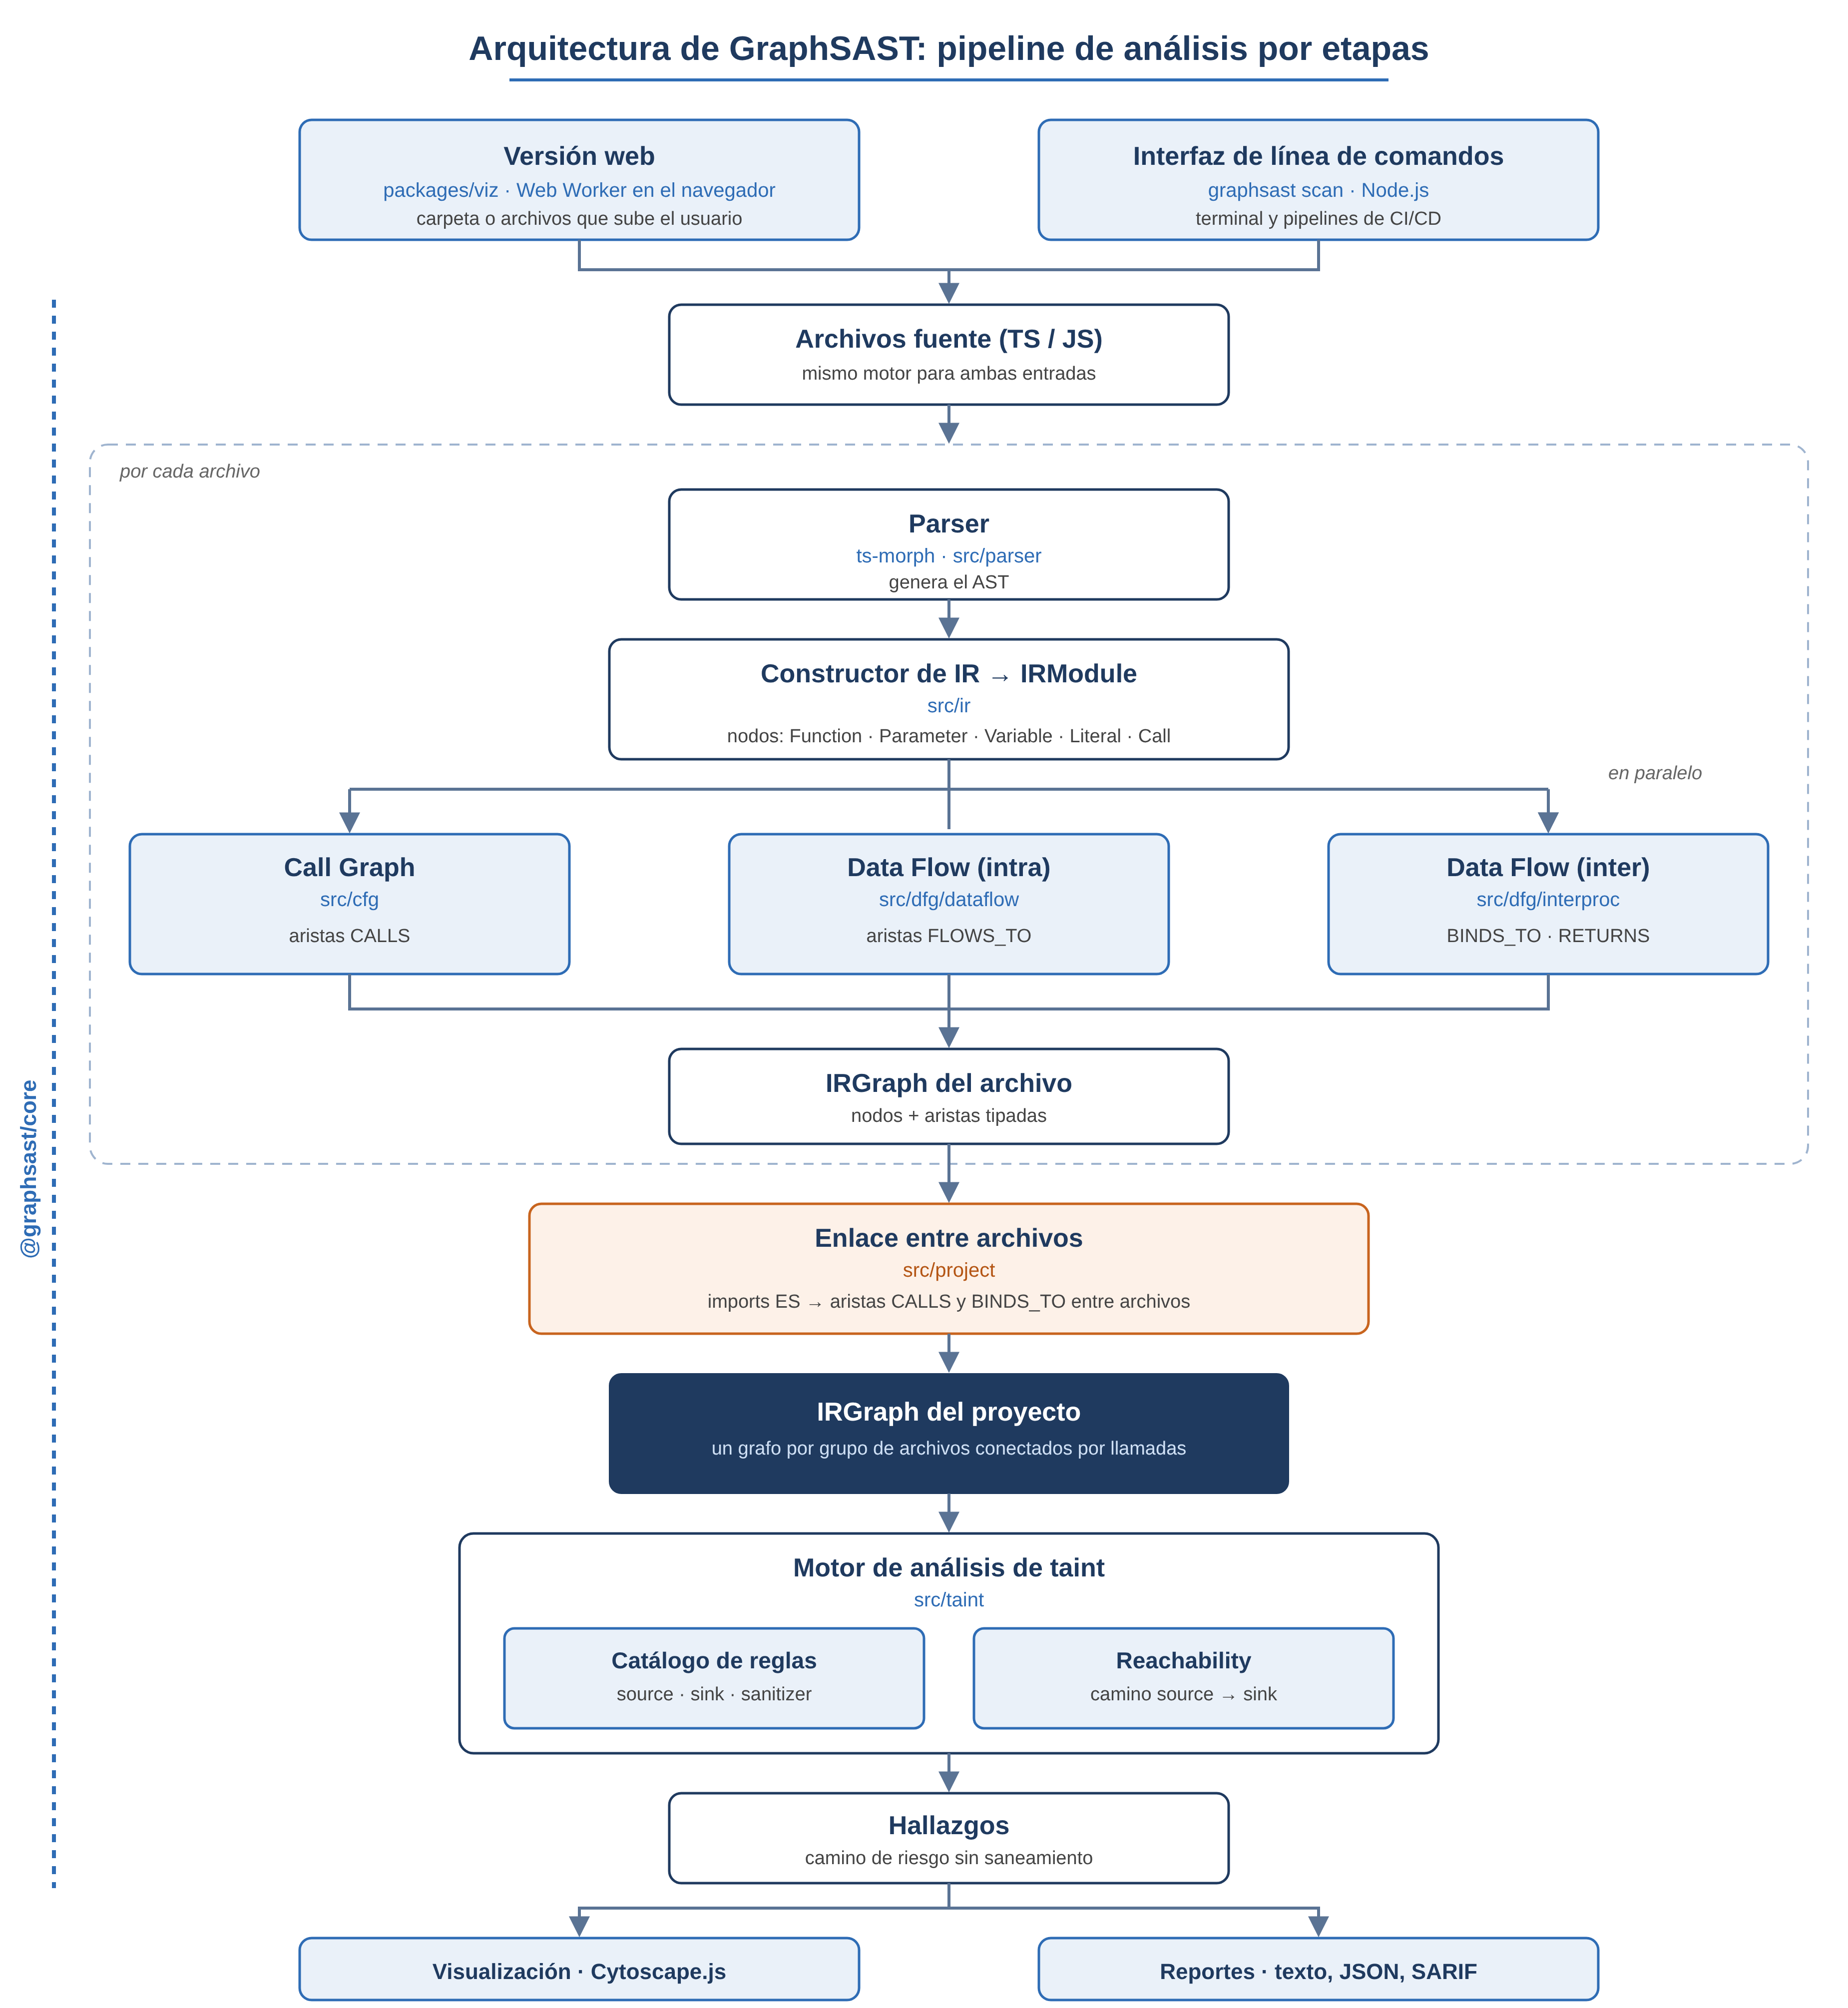
\includegraphics[width=0.7\textwidth]{figuras/arquitectura.png}
    \caption{Arquitectura de GraphSAST: pipeline de análisis por etapas, desde los archivos del proyecto hasta la visualización y los reportes, con enlace entre archivos}
    \label{fig:arquitectura}
\end{figure}

\section{Prototipo y alcance de lo construido}\label{sec:n4.2}

\subsection{Estado del desarrollo}\label{sec:n4.2.1}

El sistema se encuentra actualmente en estado de prototipo funcional. Se ejecuta como aplicación web en el navegador y procesa de forma satisfactoria los casos de prueba, aunque su alcance se define como prototipo y no como producto mínimo viable, ya que aún no fue evaluado por usuarios externos y ciertas características necesarias para su comercialización, como la gestión de suscripciones, forman parte de etapas futuras.

\subsection{Funcionalidades implementadas}\label{sec:n4.2.2}

El prototipo ejecuta el pipeline completo de análisis sobre los archivos de un proyecto: análisis sintáctico, construcción de la representación intermedia, generación del grafo de llamadas, análisis de flujo de datos intra e inter-procedural, y detección de recorridos desde puntos de entrada hacia operaciones sensibles sin saneamiento intermedio. La detección se resuelve mediante dos motores intercambiables: un recorrido en anchura sobre el grafo en memoria, empleado por defecto, y una consulta declarativa en Cypher ejecutada sobre el grafo persistido en Neo4j, que descarta los caminos que atraviesan un nodo de saneamiento y acota la profundidad de búsqueda. Los resultados se presentan mediante visualización interactiva del grafo, con resaltado del camino de riesgo y vinculación con las líneas de código correspondientes. El análisis sigue el dato de un archivo a otro cuando una función importada desde otro archivo del proyecto lo recibe como argumento. La versión web analiza una carpeta o un conjunto de archivos elegidos por el usuario, y la interfaz de línea de comandos analiza rutas del disco, emite reportes en texto, JSON y SARIF, y devuelve códigos de salida que permiten detener un pipeline de integración continua cuando se detectan hallazgos.

\subsection{Catálogo de detección}\label{sec:n4.2.3}

Se implementaron las tres debilidades definidas en el diseño arquitectónico, seleccionadas por constituir la tríada canónica del análisis de contaminación y por integrar el listado de debilidades más críticas publicado por MITRE, a las que se sumó la inyección NoSQL (CWE-943), habitual en aplicaciones Node.js que emplean bases de datos documentales como MongoDB:

\begin{table}[H]
    \centering
    \caption{Debilidades cubiertas por el catálogo de detección implementado}
    \label{tab:catalogo}
    \small
    \begin{tabularx}{\textwidth}{l L r r}
        \toprule
        \tb{Debilidad} & \tb{Descripción} & \tb{Sinks} & \tb{Sanitizers} \\
        \midrule
        CWE-89 & Inyección SQL & 5 & 5 \\
        CWE-78 & Inyección de comandos del sistema operativo & 6 & 4 \\
        CWE-79 & Cross-Site Scripting (XSS) & 6 & 5 \\
        CWE-943 & Inyección NoSQL & 6 & 4 \\
        \bottomrule
    \end{tabularx}
\end{table}

Las operaciones sensibles registradas corresponden a llamadas habituales del ecosistema analizado: controladores de bases de datos relacionales, mapeadores objeto-documento, ejecución de procesos del sistema operativo y manipulación del modelo de objetos del documento. Las operaciones de saneamiento reconocidas comprenden tanto funciones genéricas de validación y escapado como bibliotecas específicas del dominio.

\subsection{Verificación y resultados}\label{sec:n4.2.4}

El desarrollo cuenta con una suite de pruebas automatizadas organizadas según la etapa del pipeline que verifican, lo que permite validar cada componente de forma aislada. La aplicación incorpora asimismo dos casos de demostración que difieren en una sola línea: un fragmento en el que el identificador recibido en la URL cruza de una función a otra y llega a una consulta a base de datos, y el mismo fragmento con una operación de saneamiento intermedia. Los demás escenarios, como los flujos dentro de una misma función, las operaciones sensibles alcanzadas por literales, las entradas de Express, la inyección de comandos y el XSS, se cubren en el banco de pruebas descrito más adelante.

La figura siguiente presenta el análisis de un caso vulnerable. El dato ingresa por el parámetro de una función, se asigna a una variable intermedia, se transfiere como argumento a otra función y alcanza una operación de consulta a base de datos sin haber atravesado ninguna operación de saneamiento. El sistema identifica el recorrido y lo resalta sobre el grafo, indicando además las líneas de código involucradas.

\begin{figure}[H]
    \centering
    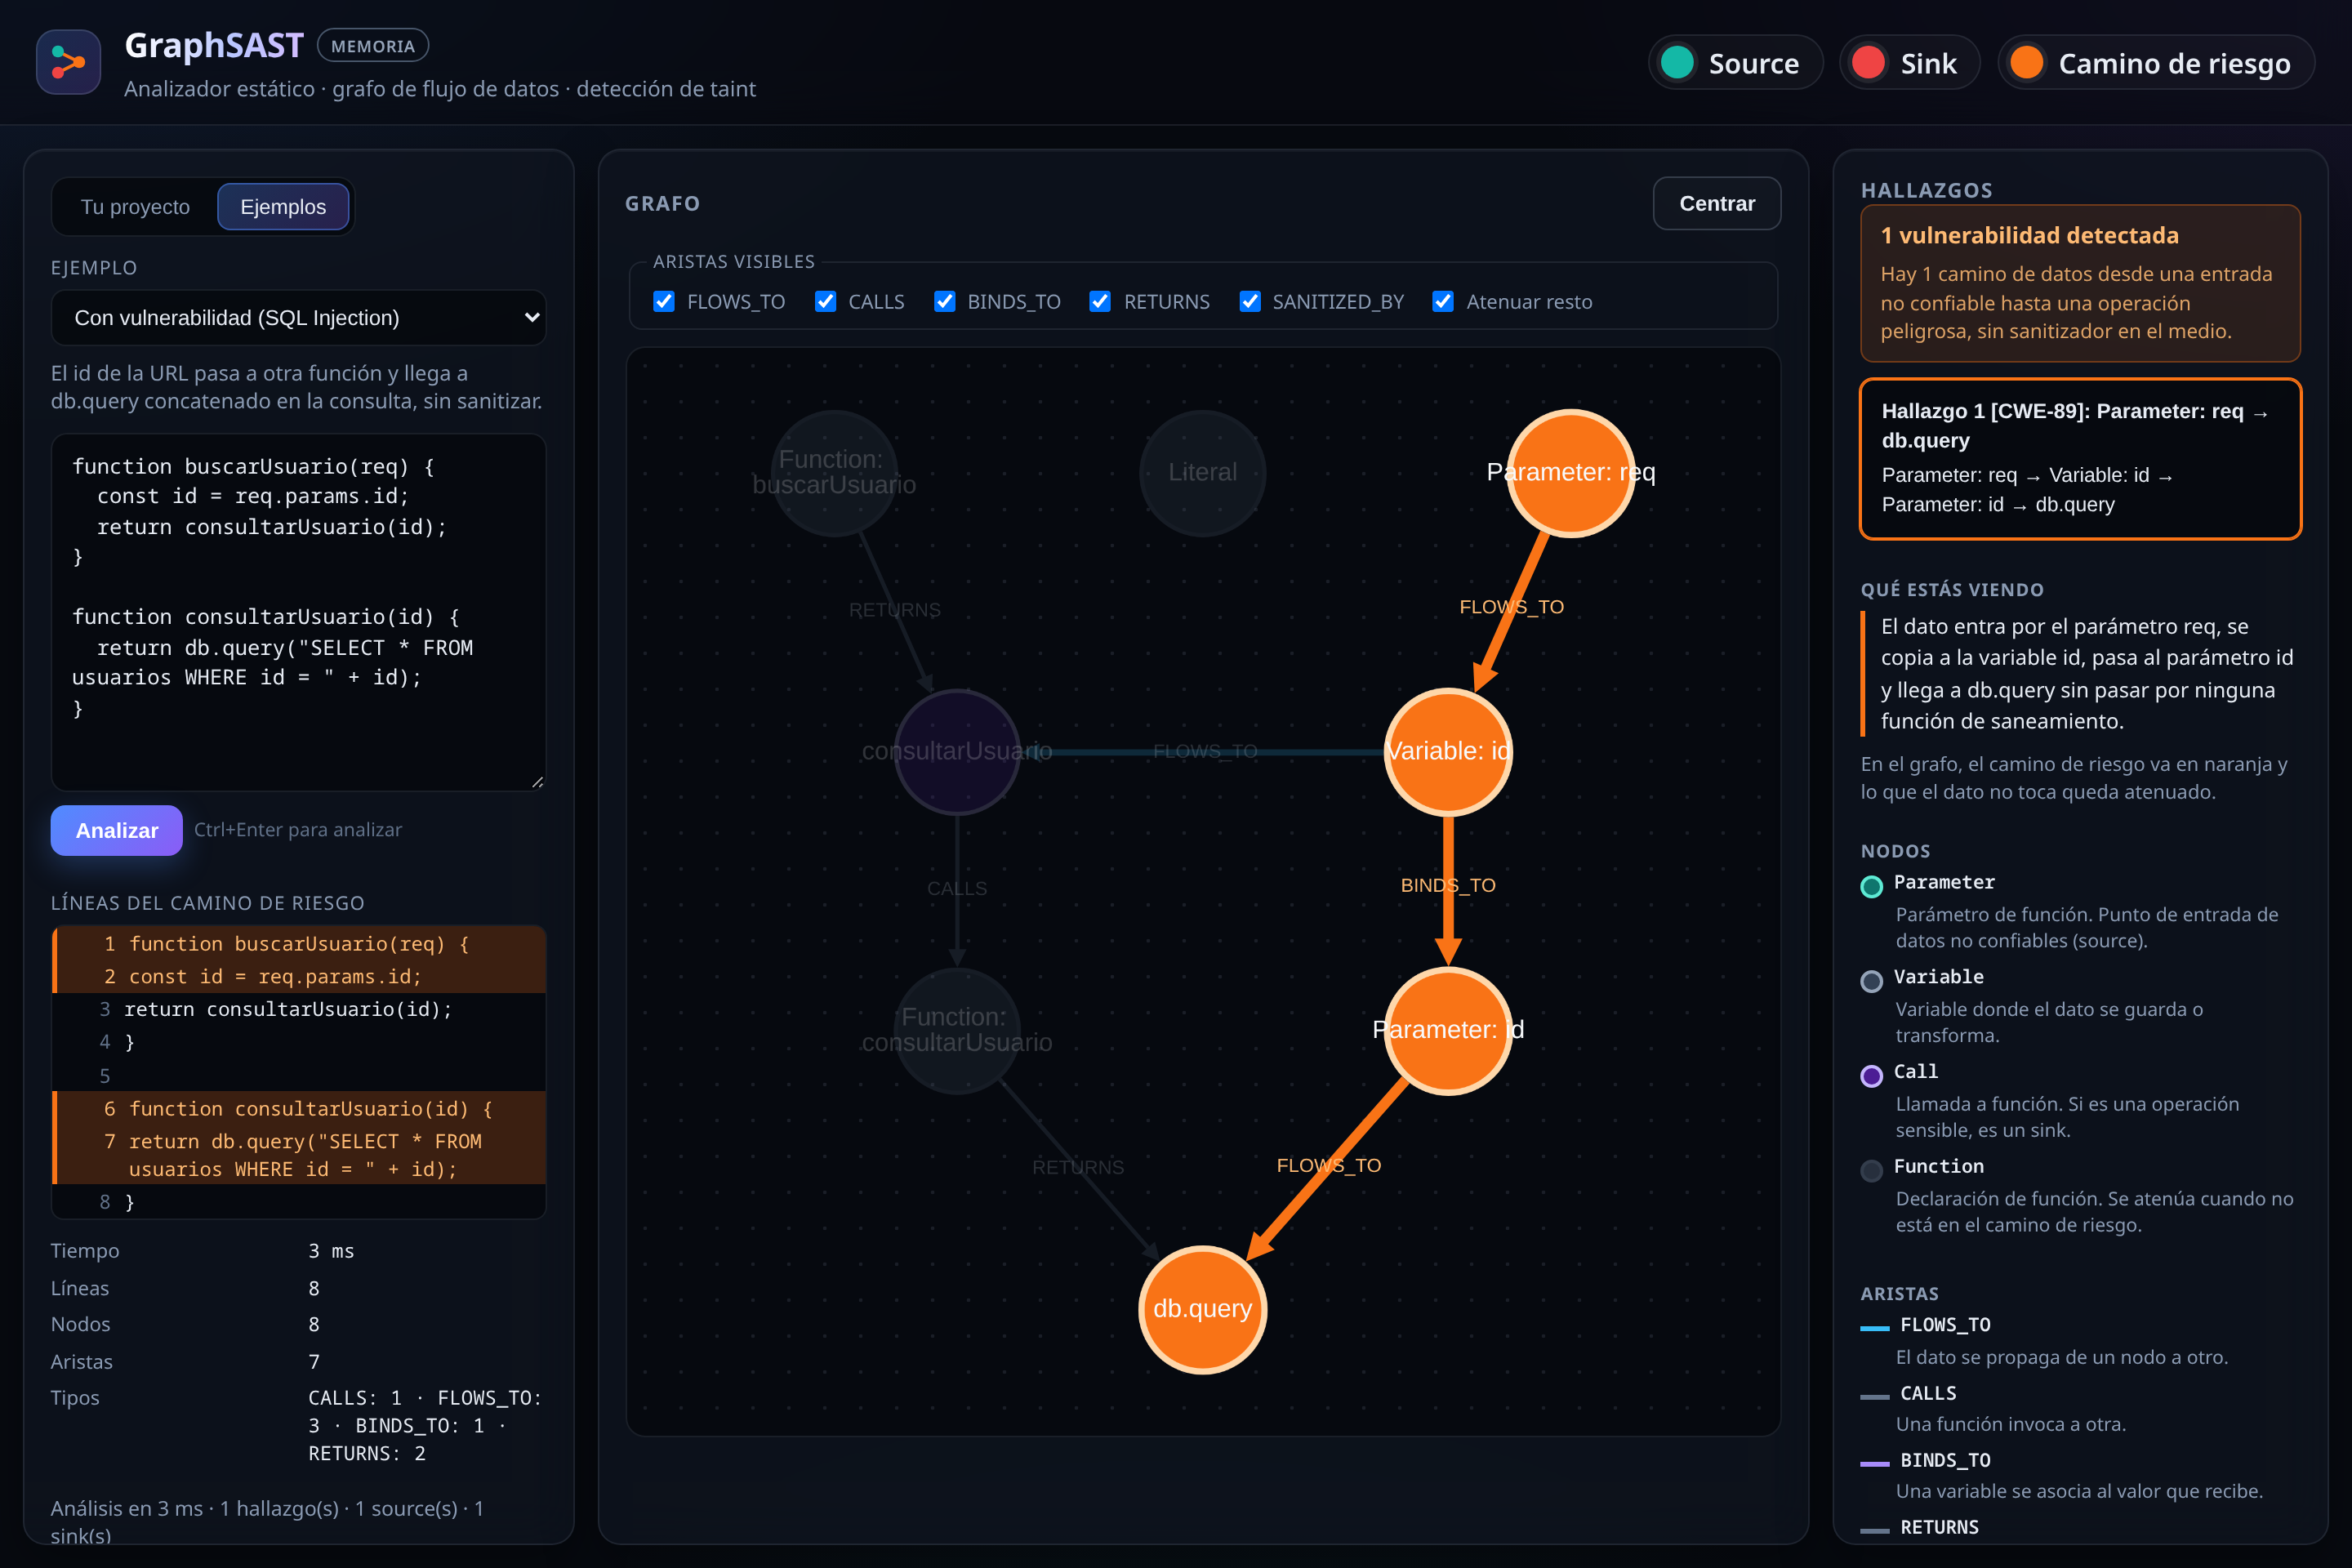
\includegraphics[width=0.9\textwidth]{figuras/deteccion.png}
    \caption{Detección de vulnerabilidad (CWE-89): el dato fluye desde el parámetro de entrada hasta la operación de consulta sin saneamiento intermedio. El camino de riesgo se resalta en la visualización}
    \label{fig:deteccion}
\end{figure}

El comportamiento ante un dato correctamente validado resulta particularmente relevante para las hipótesis del trabajo. En el caso siguiente, el mismo patrón de flujo incorpora una operación de saneamiento intermedia. El sistema reconoce la presencia de un punto de entrada y de una operación sensible —los identifica y los diferencia cromáticamente— pero descarta el hallazgo al verificar el saneamiento en el recorrido. Una herramienta basada en coincidencia de patrones señalaría la operación como vulnerable, dado que carece de la capacidad de determinar si el dato fue procesado en el trayecto.

\begin{figure}[H]
    \centering
    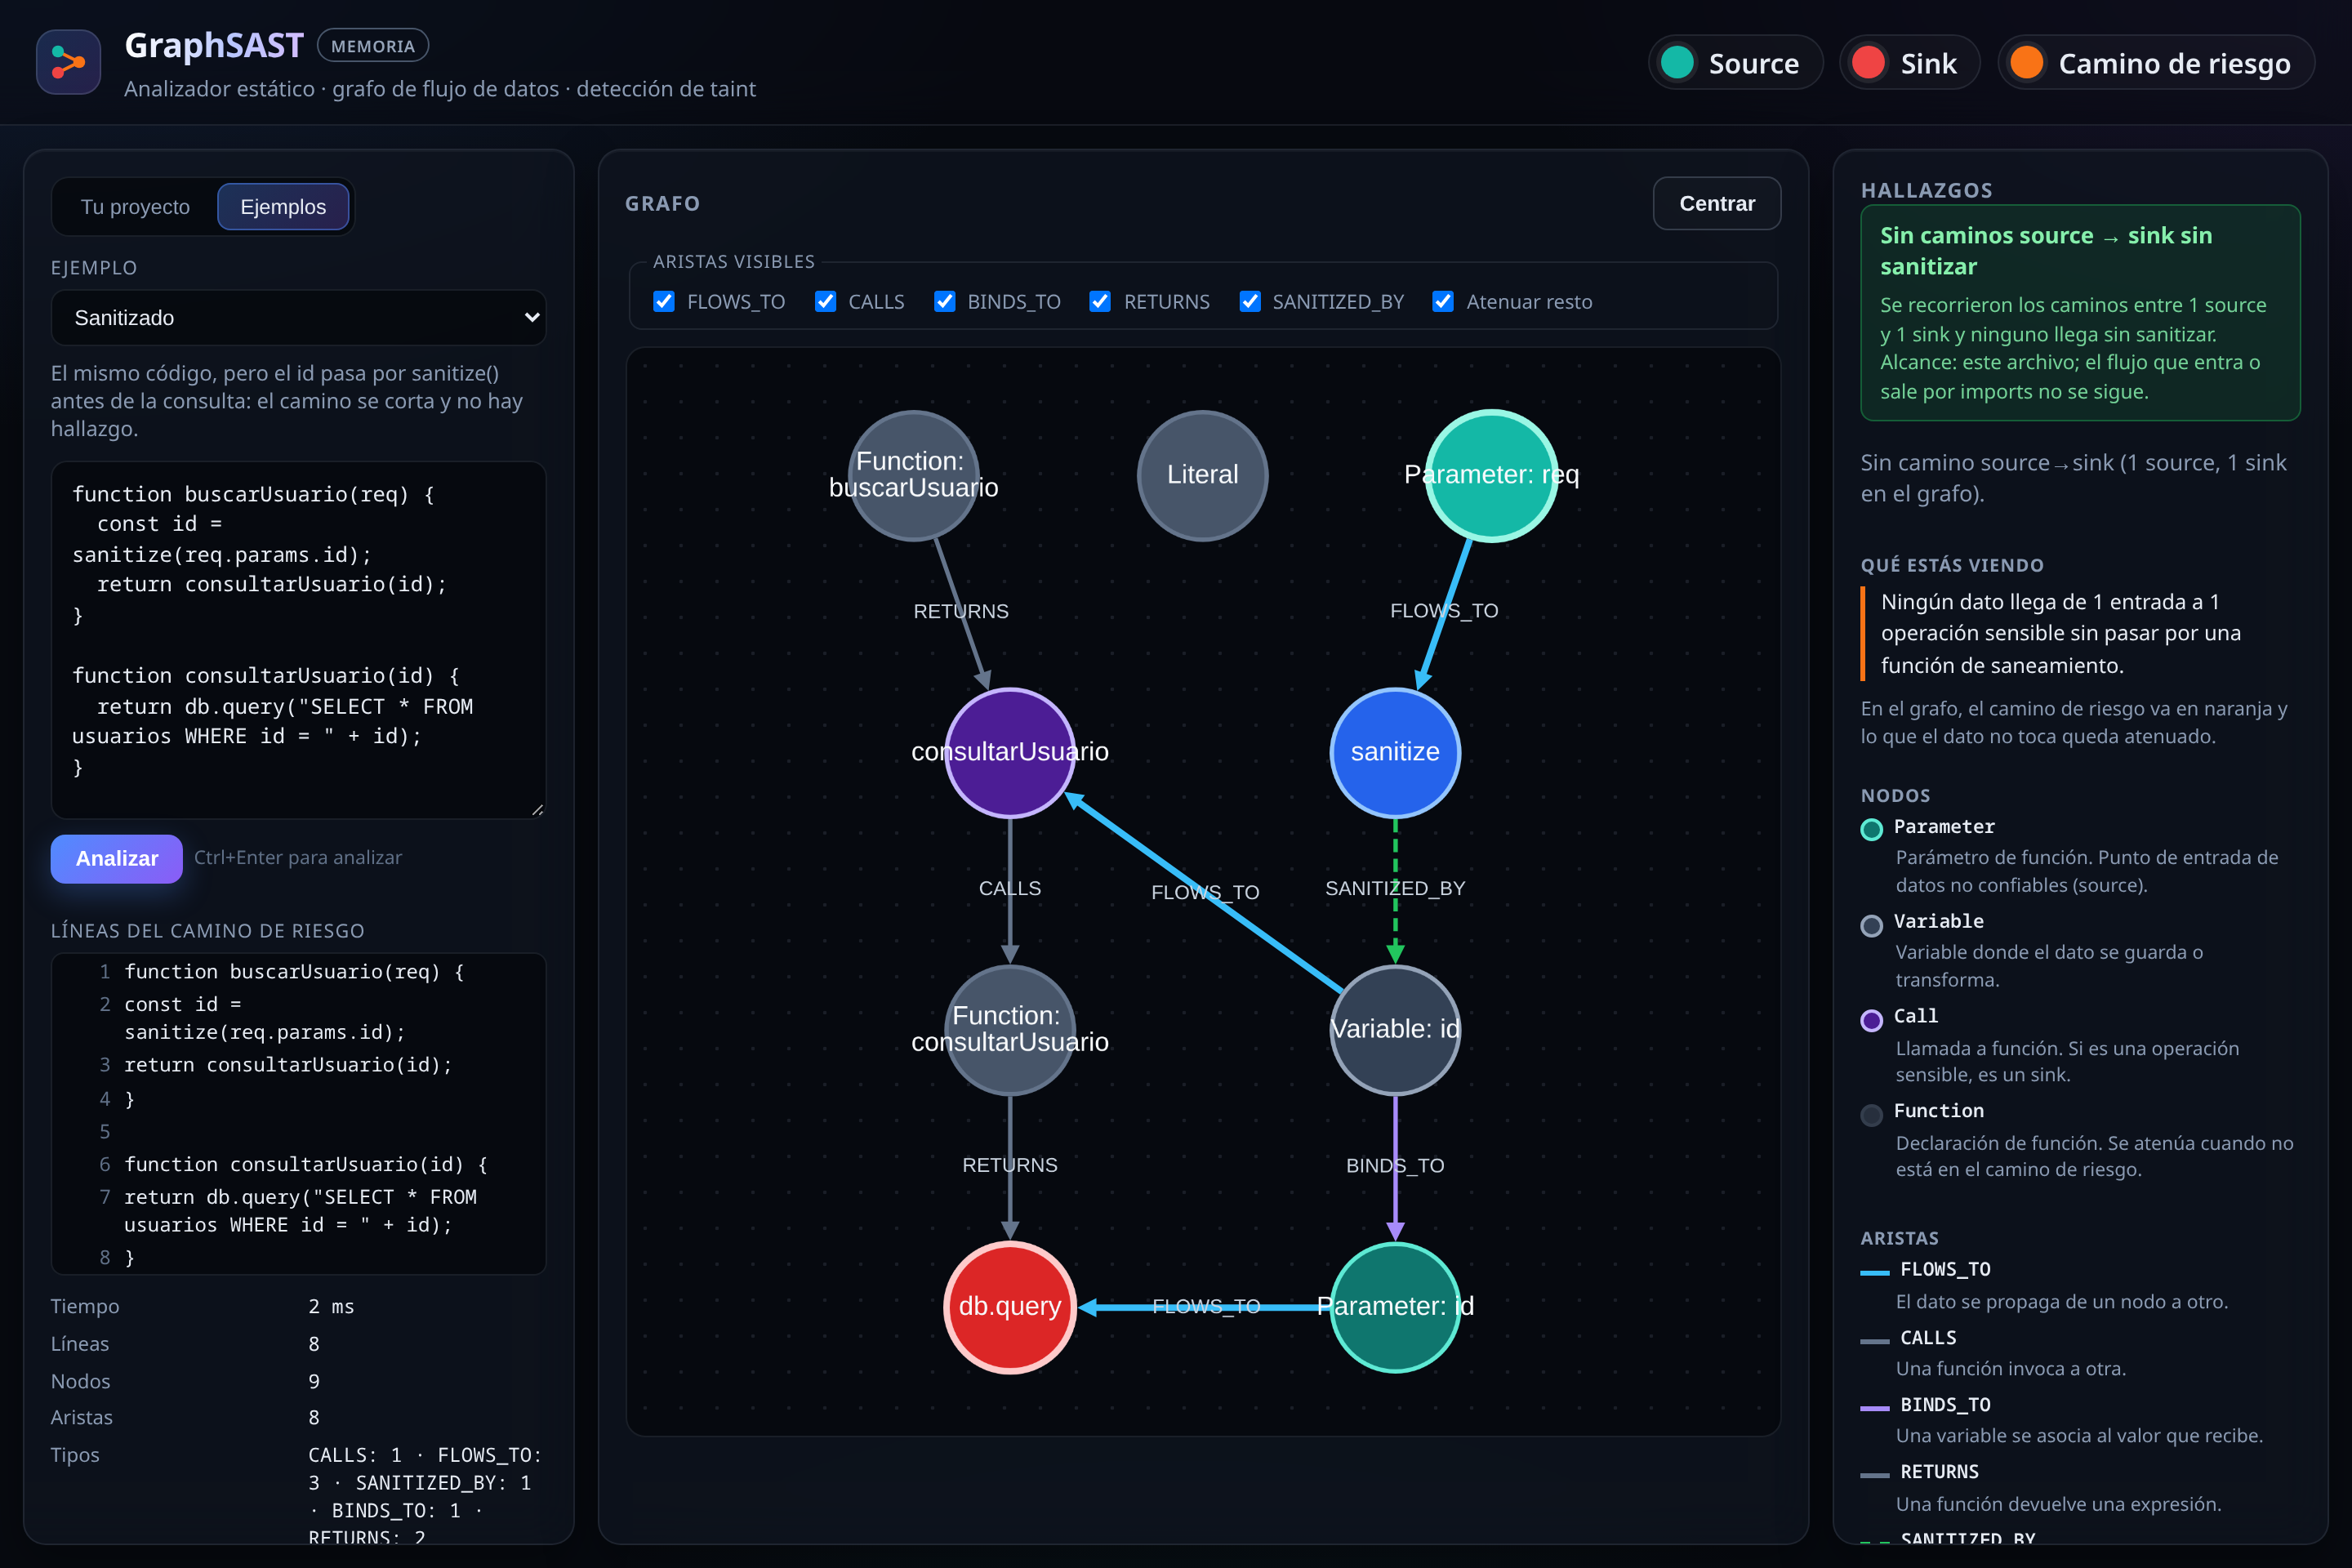
\includegraphics[width=0.9\textwidth]{figuras/saneado.png}
    \caption{Caso saneado: el mismo patrón de flujo con una operación de saneamiento intermedia. El sistema identifica el origen y el destino sensible, pero descarta el hallazgo al constatar el saneamiento en el recorrido}
    \label{fig:saneado}
\end{figure}

La interfaz expone asimismo las métricas correspondientes a cada ejecución, que incluyen el tiempo de análisis, la cantidad de líneas procesadas, y el número de nodos y aristas generados en el grafo, discriminados por tipo de relación. Los tiempos registrados sobre los casos de prueba se ubican en el orden de las decenas de milisegundos.

\begin{figure}[H]
    \centering
    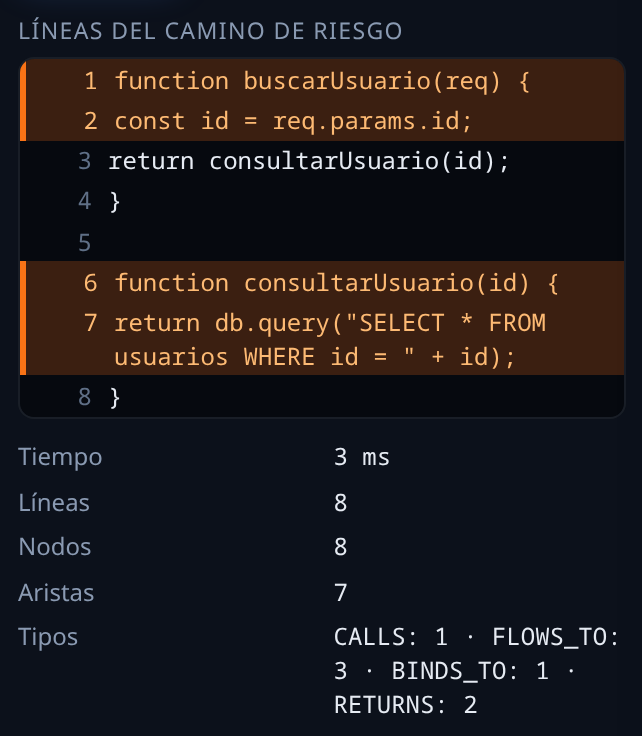
\includegraphics[width=0.5\textwidth]{figuras/metricas.png}
    \caption{Panel de métricas y líneas del camino de riesgo correspondientes al análisis ejecutado}
    \label{fig:metricas}
\end{figure}

La evaluación cuantitativa se ejecuta sobre un banco de pruebas etiquetado y reproducible desde la línea de comandos, integrado por cuarenta y tres casos de verdad conocida (veintinueve vulnerables y catorce seguros) que cubren recorridos intra e inter-procedurales, casos saneados, operaciones sensibles alcanzadas por literales constantes y entradas propias de Express. Además de las tres debilidades del catálogo, el banco incorpora casos de validación insuficiente de la entrada (CWE-20) que alcanzan operaciones sensibles ya catalogadas. Cada caso se clasifica de forma binaria según el sistema emita o no hallazgos, lo que permite construir la matriz de confusión y derivar los indicadores definidos en el Capítulo~\ref{cap:metodologia}.

\begin{table}[H]
    \centering
    \caption{Resultados del banco de pruebas sintético (43 casos; tiempos: mediana de cinco ejecuciones)}
    \label{tab:banco-sintetico}
    \small
    \begin{tabularx}{\textwidth}{L l}
        \toprule
        \tb{Indicador} & \tb{Valor obtenido} \\
        \midrule
        Verdaderos positivos (TP) & 29 \\
        Falsos positivos (FP) & 0 \\
        Verdaderos negativos (TN) & 14 \\
        Falsos negativos (FN) & 0 \\
        Precisión & 1,00 \\
        Exhaustividad (Recall) & 1,00 \\
        F1 & 1,00 \\
        Tiempo total de análisis & 52 ms \\
        Tiempo por línea de código & 0,27 ms \\
        \bottomrule
    \end{tabularx}
\end{table}

Corresponde delimitar el alcance de estos valores. Se obtienen sobre un corpus sintético reducido, construido por el propio autor y acotado a las construcciones sintácticas que el analizador cubre, por lo que no constituyen evidencia de desempeño sobre proyectos reales ni admiten generalización. Su función en esta instancia es la de una prueba de regresión que verifica que el motor no emite alertas sobre los casos correctamente saneados ni omite los recorridos vulnerables conocidos. La comparación cuantitativa con una herramienta de referencia, prevista en el diseño de investigación del Capítulo~\ref{cap:metodologia}, permanece pendiente. La validación frente a vulnerabilidades documentadas se presenta a continuación.

Para contrastar el sistema con vulnerabilidades reales se empleó un corpus de seis advisories del ecosistema npm publicados en la base de datos de advisories de GitHub, relevados el 1 de septiembre de 2026 y congelados para que la medición resulte reproducible, restringidos a las debilidades del catálogo. Para cada caso se descargan del registro de npm la versión vulnerable del paquete y la versión que corrige la falla, se analizan ambas contando solo los hallazgos de la debilidad del advisory y se registran dos resultados: si la versión vulnerable presenta hallazgos (detección) y si la corrección del mantenedor reduce su cantidad (discriminación). La discriminación constituye la evidencia fuerte, dado que indica que el hallazgo se vincula con la vulnerabilidad y no con un patrón presente en todo el paquete.

\begin{table}[H]
    \centering
    \caption{Validación sobre vulnerabilidades documentadas del ecosistema npm (6 casos)}
    \label{tab:advisories}
    \footnotesize
    \begin{tabularx}{\textwidth}{>{\hsize=1.3\hsize}L r l r c >{\hsize=.7\hsize}L}
        \toprule
        \tb{Paquete (vulnerable $\rightarrow$ corregida)} & \tb{CWE} & \tb{Advisory} & \tb{Archivos} & \tb{\makecell{Hallazgos\\(vuln. $\rightarrow$ corr.)}} & \tb{Resultado} \\
        \midrule
        @hypequery/clickhouse 2.5.0 $\rightarrow$ 2.5.1 & 89 & GHSA-6wcc-39rp-hh9p & 0 & — & Sin código fuente publicado \\
        @anthropic-ai/claude-code 2.1.162 $\rightarrow$ 2.1.163 & 78 & GHSA-7835-87q9-rgvv & 3 & 0 $\rightarrow$ 0 & No detectado \\
        sanitize-html 2.17.4 $\rightarrow$ 2.17.5 & 79 & GHSA-vccv-cmxp-4j9h & 1 & 0 $\rightarrow$ 0 & No detectado \\
        sanitize-html 2.17.6 $\rightarrow$ 2.17.7 & 79 & GHSA-g8qq-57p8-ggw5 & 1 & 0 $\rightarrow$ 0 & No detectado \\
        defuddle 0.19.0 $\rightarrow$ 0.19.1 & 79 & GHSA-jg4p-g6xj-4qmf & 0 & — & Sin código fuente publicado \\
        dompurify 3.4.12 $\rightarrow$ 3.4.13 & 79 & GHSA-55q2-fjhq-7xh7 & 7 & 1 $\rightarrow$ 1 & Detectado, sin discriminación \\
        \bottomrule
    \end{tabularx}
\end{table}

El sistema detectó uno de los seis casos (16,7 \%) y ninguno con discriminación: el único hallazgo, en DOMPurify, se mantiene en la versión corregida, por lo que no corresponde a la vulnerabilidad reportada. El análisis de los casos explica el resultado. En dos paquetes, @hypequery/clickhouse y defuddle, el registro de npm solo contiene código compilado en la carpeta dist, que el evaluador excluye por tratarse de código generado; como verificación complementaria se analizó también esa carpeta, sin cambios en la conclusión: ningún hallazgo en el primero y tres hallazgos idénticos en ambas versiones del segundo. El paquete de @anthropic-ai/claude-code publica únicamente un envoltorio de instalación. En cuanto a la naturaleza de las fallas, las de sanitize-html y DOMPurify residen en la lógica interna de esas bibliotecas de saneamiento, como la validación incompleta de esquemas de URI o la eliminación de nodos del documento, y consisten en omisiones de sus propias reglas de filtrado; la de @hypequery/clickhouse es un error en su función de escapado de parámetros; la de defuddle consiste en interpolar atributos sin escapar al construir HTML como texto, una operación que el catálogo no registra como destino sensible; y la de inyección de comandos se origina en una confusión de rutas que habilita el escape del entorno aislado. Ninguna adopta la forma de un recorrido desde una entrada no confiable hasta una operación sensible del catálogo, que es la clase de vulnerabilidad que el modelo de accesibilidad detecta.

En consecuencia, esta validación no permite afirmar la efectividad del sistema sobre código real, y tampoco la refuta: el corpus se compone de bibliotecas cuyas fallas quedan fuera del modelo de amenaza del analizador. La validación pendiente debe orientarse a aplicaciones que reciben entradas de usuario y las conducen hacia bases de datos, procesos del sistema o el documento, que es el escenario para el que la herramienta fue diseñada, y ampliar la cantidad de casos hasta admitir conclusiones cuantitativas.

\subsection{Limitaciones del alcance actual}\label{sec:n4.2.5}

\paragraph{Alcance del análisis entre archivos.} El dato se sigue de un archivo a otro cuando un archivo invoca una función declarada con function en otro archivo del proyecto e importada mediante import de módulos ES con ruta relativa. No se siguen las importaciones mediante require, las funciones flecha o asignadas a constantes, los métodos de clase, los alias de rutas de TypeScript ni los paquetes de terceros; en esos casos cada archivo se analiza por separado. Por la misma razón, las aplicaciones organizadas en clases o con funciones flecha, habituales en Express y NestJS, quedan cubiertas de forma parcial.

\paragraph{Motor de consultas por defecto.} El sistema implementa los dos motores de resolución previstos en el diseño arquitectónico: el recorrido en memoria y la consulta declarativa en Cypher sobre el grafo persistido en Neo4j. El motor sobre base de datos opera, no obstante, de manera opcional, dado que requiere una instancia activa y la configuración de la variable de entorno correspondiente; en ausencia de dicha instancia la aplicación recurre al recorrido en memoria, que constituye el modo de operación por defecto. La paridad entre ambos motores se verificó sobre casos sintéticos y no sobre proyectos de escala.

\paragraph{Validación con usuarios.} No se realizaron pruebas de usabilidad con usuarios externos, instancia requerida para la validación de la hipótesis relativa a la utilidad de la visualización.

\subsection{Próximos pasos}\label{sec:n4.2.6}

Se prevé la consolidación del motor sobre base de datos de grafos como modo de operación habitual, la ampliación del catálogo de reglas y de los patrones de llamada que resuelve el análisis entre archivos, y la integración de la interfaz de línea de comandos en pipelines de integración continua como complemento de la versión web. Esta modalidad resulta coherente con el enfoque de incorporación temprana de controles de seguridad que fundamenta el proyecto: el análisis puede ejecutarse de forma automática sobre cada cambio del código, y en ambas modalidades el código fuente no abandona la infraestructura del usuario.

\section{Stack de software}\label{sec:n4.3}

La selección de tecnologías respondió a criterios explícitos de viabilidad, adecuación al dominio y coherencia interna del stack. La tabla siguiente resume las herramientas empleadas y la capa en la que interviene cada una.

\begin{table}[H]
    \centering
    \caption{Tecnologías empleadas en el desarrollo del prototipo}
    \label{tab:stack}
    \small
    \begin{tabularx}{\textwidth}{l l l L}
        \toprule
        \tb{Tecnología} & \tb{Versión} & \tb{Capa} & \tb{Función} \\
        \midrule
        TypeScript & 5.5 & Transversal & Lenguaje del motor y de la interfaz \\
        Node.js & — & Entorno de ejecución & Ejecución del motor de análisis \\
        Web Workers & — & Ejecución & Análisis en segundo plano en el navegador \\
        ts-morph & 23.0 & Análisis sintáctico & Generación y recorrido del AST \\
        Cytoscape.js & 3.30 & Visualización & Renderizado interactivo del grafo \\
        Vite & 5.4 & Construcción & Empaquetado y servidor de desarrollo \\
        Vitest & 2.0 & Pruebas & Ejecución de la suite automatizada \\
        npm workspaces & — & Estructura & Gestión del monorepo \\
        Neo4j & 5 Community & Persistencia & Almacenamiento del grafo compilado \\
        neo4j-driver & 6.2 & Persistencia & Cliente Bolt y ejecución de consultas Cypher \\
        Docker Compose & — & Entorno & Provisión local de la instancia de Neo4j \\
        Vercel & — & Despliegue & Publicación de la aplicación web como sitio estático \\
        \bottomrule
    \end{tabularx}
\end{table}

\subsection{Estrategia de análisis sintáctico}\label{sec:n4.3.1}

Se decidió utilizar la biblioteca ts-morph en lugar de programar un analizador sintáctico propio. Desarrollar un parser completo para la gramática de TypeScript y sus continuas actualizaciones habría consumido gran parte del tiempo del proyecto sin aportar valor diferencial. El aporte de GraphSAST está en los algoritmos de construcción del grafo de flujo de datos, el análisis de taint y la visualización del riesgo.

ts-morph simplifica la interacción con el compilador oficial de TypeScript y expone una API clara para recorrer los nodos del AST, lo que reduce de manera considerable el código necesario para navegar la estructura del programa.

\subsection{Lenguaje del motor}\label{sec:n4.3.2}

El motor se implementó en TypeScript sobre Node.js. La elección responde a tres razones: permite emplear un único lenguaje a lo largo de todo el sistema, incluida la interfaz de visualización; el sistema de tipos resulta adecuado para modelar las estructuras del grafo, en las que la distinción entre categorías de nodos y de aristas es central; y el ecosistema ofrece acceso directo a las herramientas de análisis del lenguaje objetivo. Se descartó el uso de Python, dado que el tratamiento del árbol sintáctico de TypeScript resulta menos natural fuera de su propio ecosistema, así como una solución híbrida que combinara ambos entornos, por la complejidad operativa que introduciría.

\subsection{Visualización}\label{sec:n4.3.3}

La representación gráfica se implementó con Cytoscape.js, una biblioteca JavaScript orientada específicamente a la construcción y visualización interactiva de grafos en el navegador. La selección se fundamentó en un relevamiento de herramientas del área y en la consulta con desarrolladores con experiencia previa en la materia. Se consideraron asimismo Gephi e igraph, descartadas por no resultar integrables en una aplicación web: la primera constituye una aplicación de escritorio orientada a la exploración manual de grafos, y la segunda una biblioteca de análisis destinada al cómputo de métricas antes que al renderizado interactivo. Cytoscape.js provee de manera nativa los algoritmos de disposición y el modelo de nodos y aristas requeridos por el proyecto, y cuenta con adopción consolidada en contextos de investigación y análisis de grafos.

\subsection{Herramientas de construcción y pruebas}\label{sec:n4.3.4}

El módulo de visualización emplea Vite como empaquetador y servidor de desarrollo. La elección respondió a la experiencia previa con la herramienta en proyectos de características similares, criterio que reduce la curva de aprendizaje y el riesgo de configuración en un desarrollo acotado en el tiempo. Vite ofrece además soporte nativo para TypeScript y módulos ES, lo que resulta coherente con el resto del stack. Las pruebas automatizadas se ejecutan con Vitest, seleccionado por su integración directa con Vite y por compartir su configuración, evitando duplicar la infraestructura de construcción del proyecto.

\section{Infraestructura y modelo de ejecución}\label{sec:n4.4}

El sistema se distribuye como una aplicación web estática: el servidor entrega la página y el análisis se ejecuta en el navegador del usuario. No se estructura como un servicio con procesamiento en el servidor, y esta característica condiciona los requerimientos de infraestructura, que difieren de los correspondientes a un servicio alojado convencional.

\subsection{Modelo de ejecución}\label{sec:n4.4.1}

El usuario accede a la aplicación desde el navegador y selecciona la carpeta o los archivos de su proyecto. El motor de análisis, el mismo que utiliza la interfaz de línea de comandos, se ejecuta en un proceso en segundo plano del navegador (Web Worker), de modo que la interfaz permanece operativa durante el análisis. Los archivos se leen y se analizan en el equipo del usuario: el servidor de alojamiento solo entrega los archivos estáticos de la aplicación y no recibe el código analizado. Esta propiedad resulta pertinente al dominio del proyecto: dado que la herramienta procesa código fuente potencialmente sensible, el hecho de que dicho código no abandone el entorno del usuario constituye una garantía relevante. La interfaz de línea de comandos, que ejecuta el mismo motor sobre Node.js, se mantiene para su uso en terminal y en pipelines de integración continua.

\subsection{Requerimientos}\label{sec:n4.4.2}

La versión web requiere únicamente un navegador actualizado; la interfaz de línea de comandos requiere un entorno con Node.js. No se requiere hardware especializado, servicios de terceros ni infraestructura de servidores. El desarrollo y las pruebas se realizaron sobre un equipo de escritorio de características estándar.

\subsection{Disponibilidad y escalabilidad}\label{sec:n4.4.3}

Al ejecutarse el análisis en el navegador de cada usuario, el servidor no realiza procesamiento y la carga de cada análisis recae en el equipo que lo solicita, por lo que la disponibilidad y la escalabilidad se reducen a la entrega de archivos estáticos. El factor determinante del rendimiento es el tamaño del código analizado, dado que el costo computacional del análisis crece con la cantidad de nodos y aristas del grafo generado. Como referencia, en el equipo de desarrollo el análisis en el navegador de un proyecto de 78 archivos y unas 8.500 líneas demandó alrededor de 2,8 segundos. La caracterización de dicho crecimiento forma parte de las mediciones previstas en la validación del sistema.

\section{Modelo de datos: el grafo del programa}\label{sec:n4.5}

El sistema representa el programa analizado mediante un grafo dirigido en el que los nodos corresponden a los elementos por los que circula la información y las aristas a las relaciones que se establecen entre ellos. Este modelo constituye el núcleo del aporte técnico del trabajo, dado que sobre él se resuelve la detección de vulnerabilidades.

\subsection{Nodos}\label{sec:n4.5.1}

Se definen cinco categorías de nodo. Cada nodo almacena su ubicación exacta en el código fuente —archivo, línea y columna— junto con el fragmento de texto correspondiente, lo que permite vincular cualquier elemento del grafo con su posición original en el programa.

\begin{table}[H]
    \centering
    \caption{Categorías de nodo del modelo de grafo}
    \label{tab:nodos}
    \small
    \begin{tabularx}{\textwidth}{l L}
        \toprule
        \tb{Categoría} & \tb{Elemento representado} \\
        \midrule
        Function & Declaración de función \\
        Parameter & Parámetro de entrada de una función \\
        Variable & Variable declarada \\
        Literal & Valor literal presente en el código \\
        Call & Invocación a una función u operación \\
        \bottomrule
    \end{tabularx}
\end{table}

\subsection{Aristas}\label{sec:n4.5.2}

Se definen cinco categorías de relación dirigida. La distinción entre categorías resulta determinante para el funcionamiento del sistema, dado que permite diferenciar la propagación efectiva de un valor de otras relaciones estructurales del programa.

\begin{table}[H]
    \centering
    \caption{Categorías de relación del modelo de grafo}
    \label{tab:aristas}
    \small
    \begin{tabularx}{\textwidth}{l L}
        \toprule
        \tb{Relación} & \tb{Significado} \\
        \midrule
        CALLS & Una función invoca a otra \\
        FLOWS\_TO & Un valor se propaga de un nodo a otro \\
        BINDS\_TO & Una variable se asocia al valor que recibe \\
        RETURNS & Una función devuelve una expresión \\
        SANITIZED\_BY & Un valor atraviesa una operación de saneamiento \\
        \bottomrule
    \end{tabularx}
\end{table}

\subsection{Resolución de la detección sobre el modelo}\label{sec:n4.5.3}

La identificación de una vulnerabilidad se resuelve como un problema de accesibilidad sobre el grafo: se determina si existe un camino que conecte un nodo de origen con un nodo de destino sensible sin que dicho recorrido atraviese una relación de saneamiento. Esta formulación traduce el planteo conceptual del trabajo —la seguridad entendida como accesibilidad sobre un grafo dirigido— en una operación computable sobre una estructura de datos concreta.

La relación de saneamiento cumple un rol central para evitar falsas alarmas: si una variable fue validada en el trayecto, el sistema descarta el camino. Un analizador basado en coincidencia de patrones carece de esa información y debe reportar el caso como potencialmente vulnerable.

Durante la implementación de las consultas Cypher sobre Neo4j surgió una dificultad concreta con las llamadas recursivas o cíclicas entre funciones, que generaban recorridos de longitud indefinida y demoraban el motor. Para resolverlo se acotó la profundidad de búsqueda a quince saltos entre el origen y el destino. En el recorrido en memoria ese límite es el valor por defecto de un parámetro configurable, mientras que en la consulta Cypher queda fijado en el patrón de camino. La restricción evita los recorridos indefinidos sin comprometer la detección en los flujos habituales de una aplicación web: sobre el banco de pruebas de 43 casos, el análisis completo demandó alrededor de 52 ms, aproximadamente 0,27 ms por línea de código (tabla~\ref{tab:banco-sintetico}).

\section{Diseño e interacción}\label{sec:n4.6}

\subsection{Usuario destinatario}\label{sec:n4.6.1}

La herramienta está orientada a desarrolladores y analistas que requieren auditar código fuente. El diseño asume familiaridad técnica con el lenguaje analizado y con los conceptos de seguridad involucrados, por lo que privilegia la densidad informativa sobre la simplificación de la interfaz.

\subsection{Organización de la interfaz}\label{sec:n4.6.2}

La aplicación se estructura en tres paneles simultáneos. El panel izquierdo ofrece dos modos. En el modo de proyecto, el usuario elige o arrastra una carpeta o un conjunto de archivos; la aplicación informa cuántos archivos se analizan y por qué se excluyen los demás, muestra el progreso del análisis y, al finalizar, lista los archivos con su cantidad de hallazgos junto con el contenido del archivo elegido y las líneas del camino de riesgo resaltadas (figura~\ref{fig:web-proyecto}). En el modo de ejemplos, el usuario puede ingresar un fragmento mediante un editor de texto o seleccionar uno de los dos ejemplos precargados: un fragmento con una inyección SQL y el mismo fragmento con una operación de saneamiento. El panel central presenta el grafo generado. El panel de hallazgos expone el veredicto, cada hallazgo con su debilidad, su ubicación y su recorrido, el catálogo de debilidades cubiertas y las reglas activas. La disposición simultánea responde a un criterio explícito: permitir que el usuario contraste el código, su representación como grafo y los hallazgos sin necesidad de alternar entre vistas.

\begin{figure}[H]
    \centering
    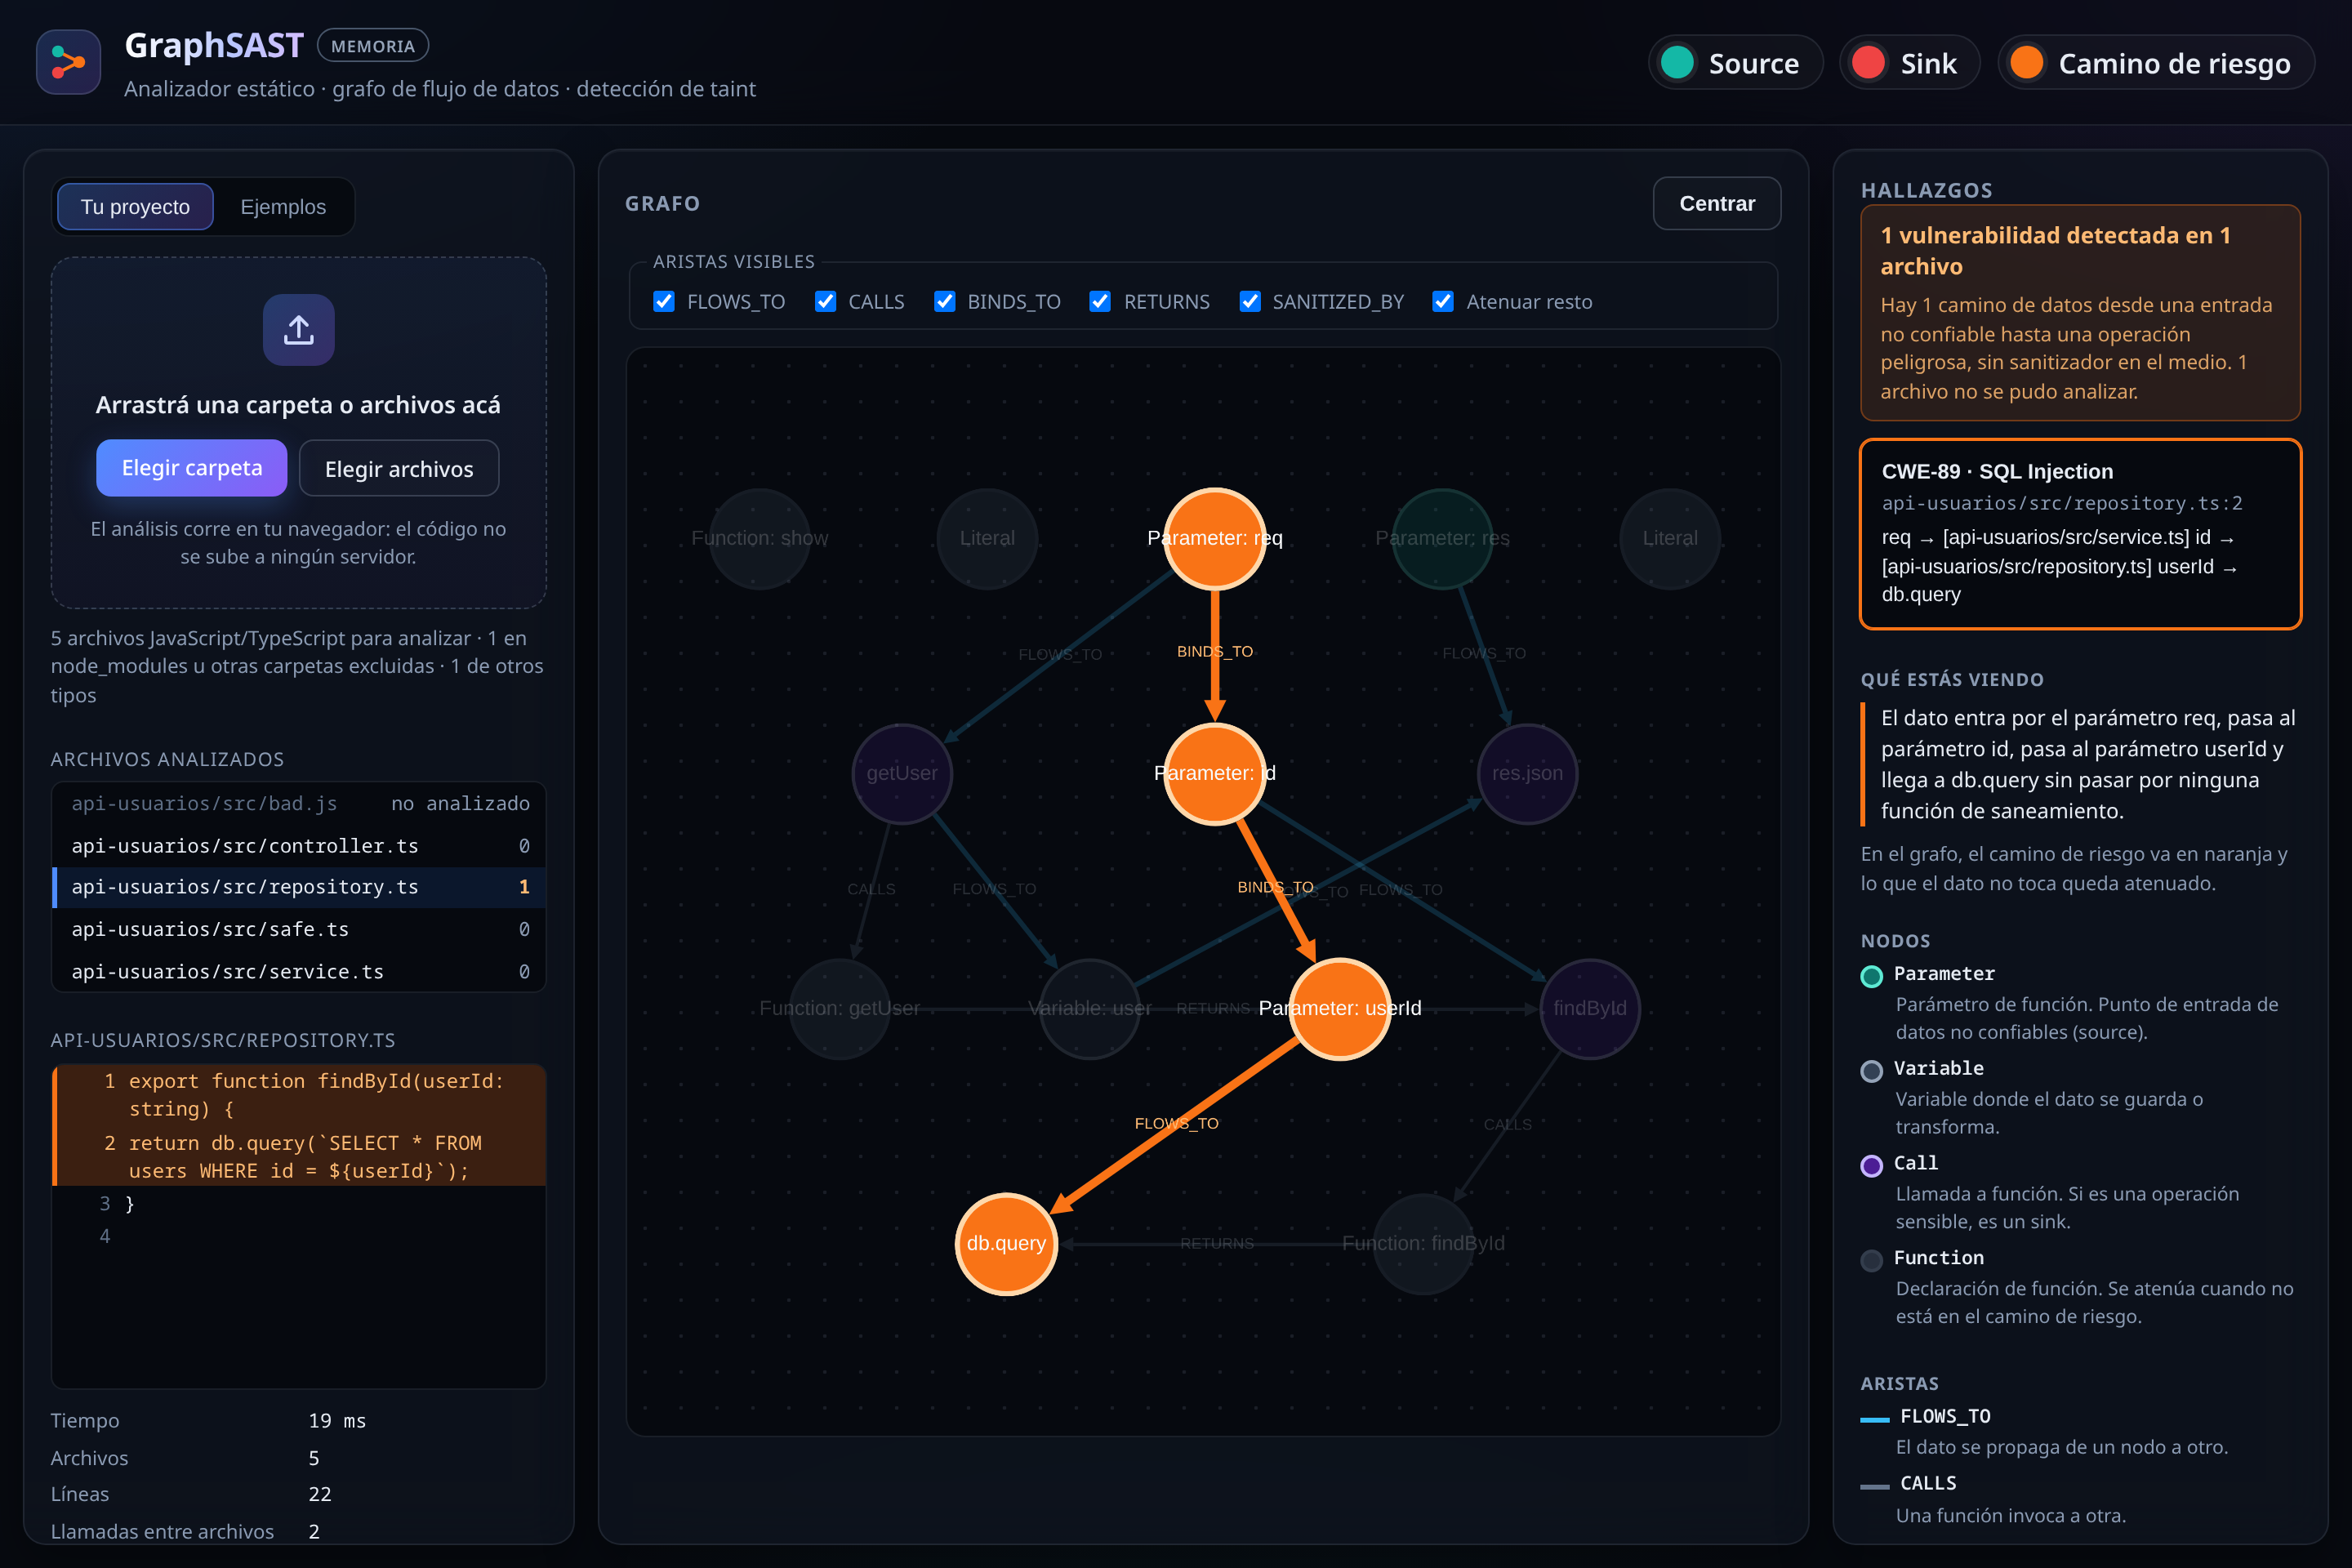
\includegraphics[width=0.9\textwidth]{figuras/web-proyecto.png}
    \caption{Versión web: análisis de un proyecto subido como carpeta. El hallazgo cruza tres archivos y se muestra el archivo del sink con las líneas del camino resaltadas}
    \label{fig:web-proyecto}
\end{figure}

\subsection{Decisiones de diseño}\label{sec:n4.6.3}

Se incorporó una codificación cromática con leyenda visible que distingue los nodos de origen, los nodos correspondientes a operaciones sensibles y el camino de riesgo identificado. Esta codificación permite interpretar el resultado de un análisis sin recurrir al texto: el contraste entre las figuras~\ref{fig:deteccion} y~\ref{fig:saneado} ilustra la diferencia entre un recorrido vulnerable y uno saneado a partir del color de los nodos y de las aristas.

El grafo admite el filtrado independiente de cada categoría de arista, junto con una opción de atenuación del resto de la estructura. Esta decisión atiende a un problema concreto de legibilidad: la superposición de relaciones de distinta naturaleza dificulta la lectura del recorrido relevante, por lo que el control sobre qué relaciones se muestran resulta necesario para interpretar grafos de cierto tamaño.

La interfaz señala además de manera explícita el modo de operación del motor mediante un indicador en el encabezado. En la versión web el análisis se resuelve siempre mediante el recorrido en memoria, dado que se ejecuta en el navegador; la consulta Cypher sobre el grafo persistido en Neo4j queda disponible a través de la API local. Esta decisión responde al criterio de que las condiciones de ejecución y las limitaciones del prototipo resulten visibles para el usuario.

\subsection{Vinculación con el código fuente}\label{sec:n4.6.4}

La interfaz presenta las líneas de código correspondientes al camino de riesgo detectado, y la selección de un nodo del grafo despliega su información asociada, incluida su ubicación en el archivo. Esta correspondencia entre la representación abstracta y el código concreto constituye el aspecto central del diseño, dado que la utilidad de la visualización depende de que el usuario pueda trasladar el hallazgo a una acción sobre el código.

\subsection{Accesibilidad y validación}\label{sec:n4.6.5}

Se incorporaron etiquetas descriptivas en los controles de la interfaz y regiones de actualización dinámica anunciables por lectores de pantalla, así como un atajo de teclado para ejecutar el análisis. No se realizaron pruebas de usabilidad con usuarios externos. La validación de la hipótesis relativa a la utilidad de la visualización requiere dicha instancia, prevista como trabajo posterior mediante sesiones de evaluación con desarrolladores.

\section{Calidad, seguridad y despliegue}\label{sec:n4.7}

\subsection{Estrategia de pruebas}\label{sec:n4.7.1}

El proyecto cuenta con una suite de pruebas automatizadas ejecutadas mediante Vitest. Las pruebas se organizan siguiendo la estructura por etapas del sistema, verificando de forma independiente el análisis sintáctico, la construcción de la representación intermedia, el grafo de llamadas, el análisis de flujo de datos, el motor de contaminación, la carga del catálogo de reglas, la generación de sentencias Cypher, la selección de motor, la construcción de informes, el análisis entre archivos y la carga de archivos de la versión web, además del módulo de visualización. La suite comprende doscientas cuarenta y siete pruebas distribuidas en veintisiete archivos. Esta organización deriva directamente de la decisión arquitectónica adoptada: la separación en etapas permite verificar cada componente de manera aislada y localizar con precisión el origen de una falla.

De modo complementario a las pruebas unitarias, la aplicación incorpora casos de demostración que reproducen patrones habituales de código y verifican el comportamiento del sistema tanto ante recorridos vulnerables como ante recorridos correctamente saneados.

\subsection{Control de versiones}\label{sec:n4.7.2}

El desarrollo se gestiona mediante Git, con repositorio alojado en GitHub: \url{https://github.com/MaxiZk/graphsast}. Los cambios se incorporan una vez verificado que la suite de pruebas se ejecuta satisfactoriamente y que la aplicación opera conforme a lo esperado, criterio que mantiene el repositorio en un estado funcional a lo largo del desarrollo.

\subsection{Consideraciones de seguridad}\label{sec:n4.7.3}

El sistema no administra cuentas de usuario, credenciales ni bases de datos remotas, por lo que no requiere esquemas de autenticación ni cifrado de datos en reposo. Una decisión clave del modelo de ejecución es que el código fuente analizado nunca se transmite fuera de la computadora del usuario: aunque la aplicación se sirve desde un servidor, el análisis se realiza en el navegador. Tratándose de código que puede contener vulnerabilidades o lógica propietaria, esa ejecución local elimina el riesgo de filtración hacia servidores externos.

\subsection{Despliegue}\label{sec:n4.7.4}

La aplicación web se publica como sitio estático en la plataforma Vercel, en \url{https://graph-sast.vercel.app/}. Vercel compila el proyecto a partir del repositorio y sirve los archivos resultantes sin funciones de servidor; se verificó sobre el sitio publicado que el análisis no genera solicitudes hacia otros dominios, de modo que el código analizado no sale del navegador. Para el desarrollo local, la ejecución requiere la instalación de las dependencias mediante el gestor de paquetes y la puesta en marcha del servidor de desarrollo.

    %!TEX root = ../main.tex
% =============================================================
%  CAPÍTULO 5 — JUSTIFICACIÓN ECONÓMICA (Entrega 5 · 15 % · 15/9)
% =============================================================

\chapter{Justificación económica}\label{cap:economica}

\begin{guia}[Guía de la cátedra: qué se evalúa en este capítulo]
Es el capítulo de mayor peso individual (15\,\%). Se evalúa como una
evaluación de proyectos de inversión:
\begin{enumerate}
    \item \textbf{Análisis de mercado y competidores}: tamaño, segmentos,
          precios de referencia.
    \item \textbf{Modelo de negocio}: B2B, B2C, B2G o interno; niveles de
          precio y fuentes de ingreso.
    \item \textbf{Inversión inicial} desglosada por rol y tiempo, más
          infraestructura.
    \item \textbf{Costos operativos} recurrentes.
    \item \textbf{Escenarios} pesimista, base y optimista, con flujo de caja
          proyectado a 3 a 5 años.
    \item \textbf{Indicadores}: \gls{van}, \gls{tir} y período de repago,
          con una tasa de descuento construida y justificada con fuentes.
    \item \textbf{Supuestos y restricciones} explícitos.
\end{enumerate}
Todo número con su origen: cotización, tarifa pública, estadística
citada o estimación propia declarada como tal.
\end{guia}

\section{Escenario de comercialización}\label{sec:n5.1}

El proyecto se evalúa bajo un modelo de suscripción, distribuido como aplicación web en la que el análisis se ejecuta en el navegador del usuario, complementada por una herramienta de línea de comandos (CLI) integrable en pipelines de integración y despliegue continuos. El abono mensual se fijó en USD 8 por usuario, equivalente a USD 96 anuales bajo facturación anualizada.

\subsection{Suscripción frente a licencia perpetua}\label{sec:n5.1.1}

La elección de la suscripción responde a dos motivos, uno financiero y otro técnico:

\paragraph{Recurrencia frente a esfuerzo continuo de reposición.} La suscripción genera un flujo de fondos predecible, en el que los usuarios captados continúan aportando en los ejercicios posteriores mientras utilicen la herramienta. Un esquema de licencia única obligaría a captar un volumen equivalente de clientes nuevos cada año solo para sostener el nivel de ingresos. A ello se suma que una herramienta de análisis estático demanda actualización periódica de reglas para cubrir nuevos patrones de vulnerabilidad y versiones de librerías, tarea de mantenimiento que se financia de manera natural con ingresos periódicos.

\paragraph{Inconsistencia de precios relativos.} A USD 8 por mes, un cliente iguala en cinco meses el valor típico de una licencia perpetua individual, estimada en torno a USD 50. Ofrecer ambas modalidades en paralelo a esos valores generaría arbitraje en contra de la suscripción, o exigiría fijar la licencia perpetua a un precio fuera de mercado.

\subsection{Público objetivo}\label{sec:n5.1.2}

El producto se orienta a tres segmentos:

\paragraph{Desarrolladores independientes.} Programadores de JavaScript y TypeScript, en entornos Node.js, Express y React, que necesitan auditar código fuente localmente para prevenir inyecciones SQL (CWE-89), inyecciones de comandos del sistema operativo (CWE-78) y Cross-Site Scripting (CWE-79) antes de enviar cambios al repositorio.

\paragraph{Equipos de desarrollo en PyMEs y empresas de reciente creación.} Grupos de tres a quince desarrolladores que buscan implementar prácticas de seguridad temprana sin la carga presupuestaria ni la infraestructura que requieren las suites corporativas.

\paragraph{Consultores de aseguramiento de calidad y seguridad de aplicaciones.} Profesionales que realizan auditorías puntuales sobre código de terceros.

\subsection{Relación entre público y precio}\label{sec:n5.1.3}

Las soluciones corporativas consolidadas del mercado operan con contratos anuales de miles de dólares y requieren servidores dedicados. Frente a ellas, USD 8 mensuales equivalen aproximadamente a una hora de desarrollo junior en Argentina, según la tarifa de referencia adoptada en la sección~\ref{sec:n5.2}. Ese orden de magnitud elimina la barrera de entrada para un profesional independiente o para el responsable técnico de una empresa pequeña, dado que la decisión de compra no requiere aprobaciones presupuestarias complejas.

\subsection{Dimensionamiento del mercado}\label{sec:n5.1.4}

\paragraph{Mercado total direccionable.} El relevamiento global de SlashData (State of the Developer Nation) y el reporte anual GitHub Octoverse ubican a JavaScript y TypeScript de forma constante a la cabeza del ranking de adopción, con una base mundial superior a los veinte millones de programadores. La distribución como aplicación web, accesible desde el navegador sin instalación, junto con la publicación de la herramienta de línea de comandos en el registro de paquetes npm, canal habitual de las herramientas de desarrollo del ecosistema JavaScript, permite alcanzar esa base sin intermediarios comerciales.

\paragraph{Mercado disponible regional.} Para dimensionar el mercado local se parte del dato publicado por el Observatorio Permanente de la Industria del Software y Servicios Informáticos (OPSSI) de CESSI, que registra 162.598 puestos de trabajo formales en el sector al primer trimestre de 2026. Dado que esa cifra comprende la totalidad de las funciones de las empresas —gestión, soporte, infraestructura y administración—, la proporción estrictamente técnica se estima a partir de los relevamientos de la Encuesta de Sueldos de Sysarmy, en los que los roles de desarrollo concentran entre el 50 \% y el 60 \% del personal técnico. Asumiendo de forma conservadora que entre un 35 \% y un 50 \% de ese personal de desarrollo trabaja sobre aplicaciones web en el ecosistema JavaScript/TypeScript, el mercado accesible local se ubica en un orden de entre 28.000 y 49.000 desarrolladores.

\paragraph{Mercado objetivo.} La proyección contempla alcanzar 20 usuarios en el primer año y escalar gradualmente hasta 300 usuarios activos en el quinto. Sobre el mercado accesible estimado, esos 300 suscriptores representan una cuota de penetración de entre el 0,6 \% y el 1,1 \%, lo que muestra que la factibilidad del flujo no descansa en metas de captación desmedidas.

\section{Inversión inicial}\label{sec:n5.2}

La inversión comprende las horas de ingeniería y los desembolsos requeridos para transformar el prototipo funcional en un producto comercializable: la aplicación web con cobro de suscripciones y acceso controlado por licencia.

\subsection{Supuestos de la estimación de horas}\label{sec:n5.2.1}

Los parámetros de dedicación correspondientes a la fase de prototipo y a las tareas pendientes hasta el lanzamiento se resumen en la tabla~\ref{tab:supuestos-horas}.

\begin{table}[H]
    \centering
    \caption{Supuestos de estimación de horas de desarrollo}
    \label{tab:supuestos-horas}
    \small
    \begin{tabularx}{\textwidth}{L L}
        \toprule
        \tb{Parámetro} & \tb{Valor adoptado} \\
        \midrule
        Período de desarrollo del prototipo & Mediados de junio a mediados de septiembre de 2026 (13 semanas) \\
        Días dedicados por semana & 3 a 4 días (promedio: 3,5) \\
        Horas diarias de trabajo & 4 a 5 horas (promedio: 4,5) \\
        Carga semanal estimada & $\approx$ 15,75 horas \\
        Horas insumidas en el prototipo & $\approx$ 205 horas (rango representativo: 156 a 260) \\
        Horas adicionales hasta producto comercializable & 400 horas (cobro de suscripciones y emisión de licencias, control de acceso en la aplicación web, publicación de la herramienta de línea de comandos en npm, documentación y pruebas con usuarios) \\
        \bottomrule
    \end{tabularx}
\end{table}

\subsection{Determinación del valor hora}\label{sec:n5.2.2}

Se adoptó un valor de USD 8 por hora como costo total para el empleador. La cifra se construye en tres pasos. La Encuesta de Sueldos 2026.01 de Sysarmy, analizada por OpenQube, reporta para la categoría Junior en Argentina una mediana salarial bruta de ARS 1.538.500 mensuales; sobre un estándar de 160 horas laborales mensuales, ello equivale a ARS 9.616 por hora de salario bruto. A dicho valor corresponde adicionar las contribuciones patronales y cargas sociales, que en el régimen argentino incrementan el costo laboral en aproximadamente un 25 \% respecto del salario bruto, con lo que el costo por hora asciende a ARS 12.020. Convertido al tipo de cambio mayorista de referencia indicado en la sección~\ref{sec:n5.4}, el valor resultante se ubica en el orden de USD 8 por hora.

Se emplea el costo total para el empleador, y no el salario bruto percibido, por tratarse de la magnitud que refleja el verdadero consumo de recursos que implica cada hora de desarrollo.

\subsection{Composición de la inversión inicial}\label{sec:n5.2.3}

En la tabla~\ref{tab:inversion} se detallan las erogaciones previstas para el Año 0.

\begin{table}[H]
    \centering
    \caption{Presupuesto de inversión inicial (Año 0)}
    \label{tab:inversion}
    \small
    \begin{tabularx}{\textwidth}{L L r}
        \toprule
        \tb{Concepto} & \tb{Cálculo} & \tb{Importe (USD)} \\
        \midrule
        Desarrollo del prototipo & 205 h $\times$ USD 8 & 1.640 \\
        Desarrollo hasta versión comercializable & 400 h $\times$ USD 8 & 3.200 \\
        Marketing y lanzamiento inicial & Sitio informativo, registro y difusión & 500 \\
        Licencias de software & Pila tecnológica de código abierto & 0 \\
        Hardware y equipamiento & Equipo informático propio disponible & 0 \\
        Infraestructura de servidores & Plan gratuito de Vercel durante el desarrollo, sin uso comercial & 0 \\
        Total inversión inicial (Año 0) &  & 5.340 \\
        \bottomrule
    \end{tabularx}
\end{table}

\section{Costos post-proyecto}\label{sec:n5.3}

Los costos operativos anuales necesarios para sostener la herramienta durante el horizonte de cinco años comprenden tres componentes.

El primero corresponde al mantenimiento técnico y al soporte. Se estiman seis horas mensuales destinadas a la atención de incidencias, la corrección de errores y la actualización del catálogo de reglas, valorizadas al costo horario adoptado, lo que arroja un costo anual fijo de USD 576.

El segundo corresponde al alojamiento y al dominio. La aplicación web se publica en Vercel, cuyo plan gratuito se limita al uso personal no comercial; la comercialización exige el plan Pro, con un abono fijo de USD 20 mensuales (USD 240 anuales) que incluye 1 TB mensual de transferencia de datos, volumen holgado para una aplicación estática cuyo análisis se ejecuta en el navegador. La validación de las licencias se resuelve con una función de servidor de consumo marginal, cuyo excedente sobre el uso incluido en el plan se factura a USD 0,60 por millón de invocaciones. La renovación del dominio .com cuesta USD 11,25 anuales en el registrador de Vercel, redondeados a USD 11.

El tercero corresponde a las comisiones de cobro. El cobro de las suscripciones y la emisión de licencias se delegan en Lemon Squeezy, que actúa como comerciante registrado (merchant of record): procesa los pagos, liquida los impuestos al consumo de cada país y emite claves de licencia que vencen junto con la suscripción, por lo que la aplicación no necesita administrar cuentas de usuario propias. Su comisión es del 5 \% más USD 0,50 por transacción, sin cargo mensual; Paddle, alternativa equivalente, aplica la misma tarifa. Con facturación anual, cada suscriptor genera una transacción de USD 96 y una comisión de USD 5,30, de modo que este rubro crece con la base de usuarios.

\begin{table}[H]
    \centering
    \caption{Costos operativos anuales post-proyecto, en dólares (Años 1 a 5)}
    \label{tab:costos-operativos}
    \small
    \begin{tabularx}{\textwidth}{L r r r r r}
        \toprule
        \tb{Rubro} & \tb{Año 1} & \tb{Año 2} & \tb{Año 3} & \tb{Año 4} & \tb{Año 5} \\
        \midrule
        Mantenimiento y soporte & 576 & 576 & 576 & 576 & 576 \\
        Alojamiento (Vercel Pro) & 240 & 240 & 240 & 240 & 240 \\
        Dominio & 11 & 11 & 11 & 11 & 11 \\
        Comisiones de cobro & 106 & 318 & 636 & 1.060 & 1.590 \\
        Costo operativo total anual & 933 & 1.145 & 1.463 & 1.887 & 2.417 \\
        \bottomrule
    \end{tabularx}
\end{table}

\section{Flujo de fondos proyectado}\label{sec:n5.4}

\subsection{Supuestos del flujo}\label{sec:n5.4.1}

\paragraph{Moneda de cuenta.} La totalidad del flujo se expresa en dólares estadounidenses, con el objeto de aislar la proyección del efecto de la inflación en moneda local. Como referencia para los costos originados en pesos se tomó el tipo de cambio mayorista de la Comunicación «A» 3500 del Banco Central de la República Argentina, que al 11 de septiembre de 2026 se ubicó en ARS 1.509,91 por dólar.

\paragraph{Ingreso por usuario.} Cada suscriptor activo abona USD 96 por año en un único pago anual, equivalentes a USD 8 mensuales. Los impuestos al consumo que liquida el procesador de pagos se suman al precio y no forman parte del ingreso.

\paragraph{Adopción progresiva.} 20 usuarios en el primer año, 60 en el segundo, 120 en el tercero, 200 en el cuarto y 300 en el quinto.

\paragraph{Cómputo temporal.} La inversión se efectúa en el momento inicial (Año 0), mientras que los cobros y los costos operativos se imputan al cierre de cada ejercicio anual.

\begin{table}[H]
    \centering
    \caption{Flujo de fondos proyectado, en dólares (Años 0 a 5)}
    \label{tab:flujo-caja}
    \small
    \begin{tabularx}{\textwidth}{l r r r r L}
        \toprule
        \tb{Año} & \tb{Usuarios} & \tb{Ingresos} & \tb{Costos} & \tb{Flujo neto} & \tb{Flujo acumulado} \\
        \midrule
        0 & — & — & — & $-$5.340 & $-$5.340 \\
        1 & 20 & 1.920 & $-$933 & 987 & $-$4.353 \\
        2 & 60 & 5.760 & $-$1.145 & 4.615 & 262 \\
        3 & 120 & 11.520 & $-$1.463 & 10.057 & 10.319 \\
        4 & 200 & 19.200 & $-$1.887 & 17.313 & 27.632 \\
        5 & 300 & 28.800 & $-$2.417 & 26.383 & 54.015 \\
        Total &  & 67.200 & $-$7.845 & 54.015 &  \\
        \bottomrule
    \end{tabularx}
\end{table}

La figura~\ref{fig:flujo-fondos} representa el mismo flujo: las barras corresponden al flujo neto de cada año y la línea, al acumulado, que cruza el cero a los 1,94 años.

\begin{figure}[H]
    \centering
    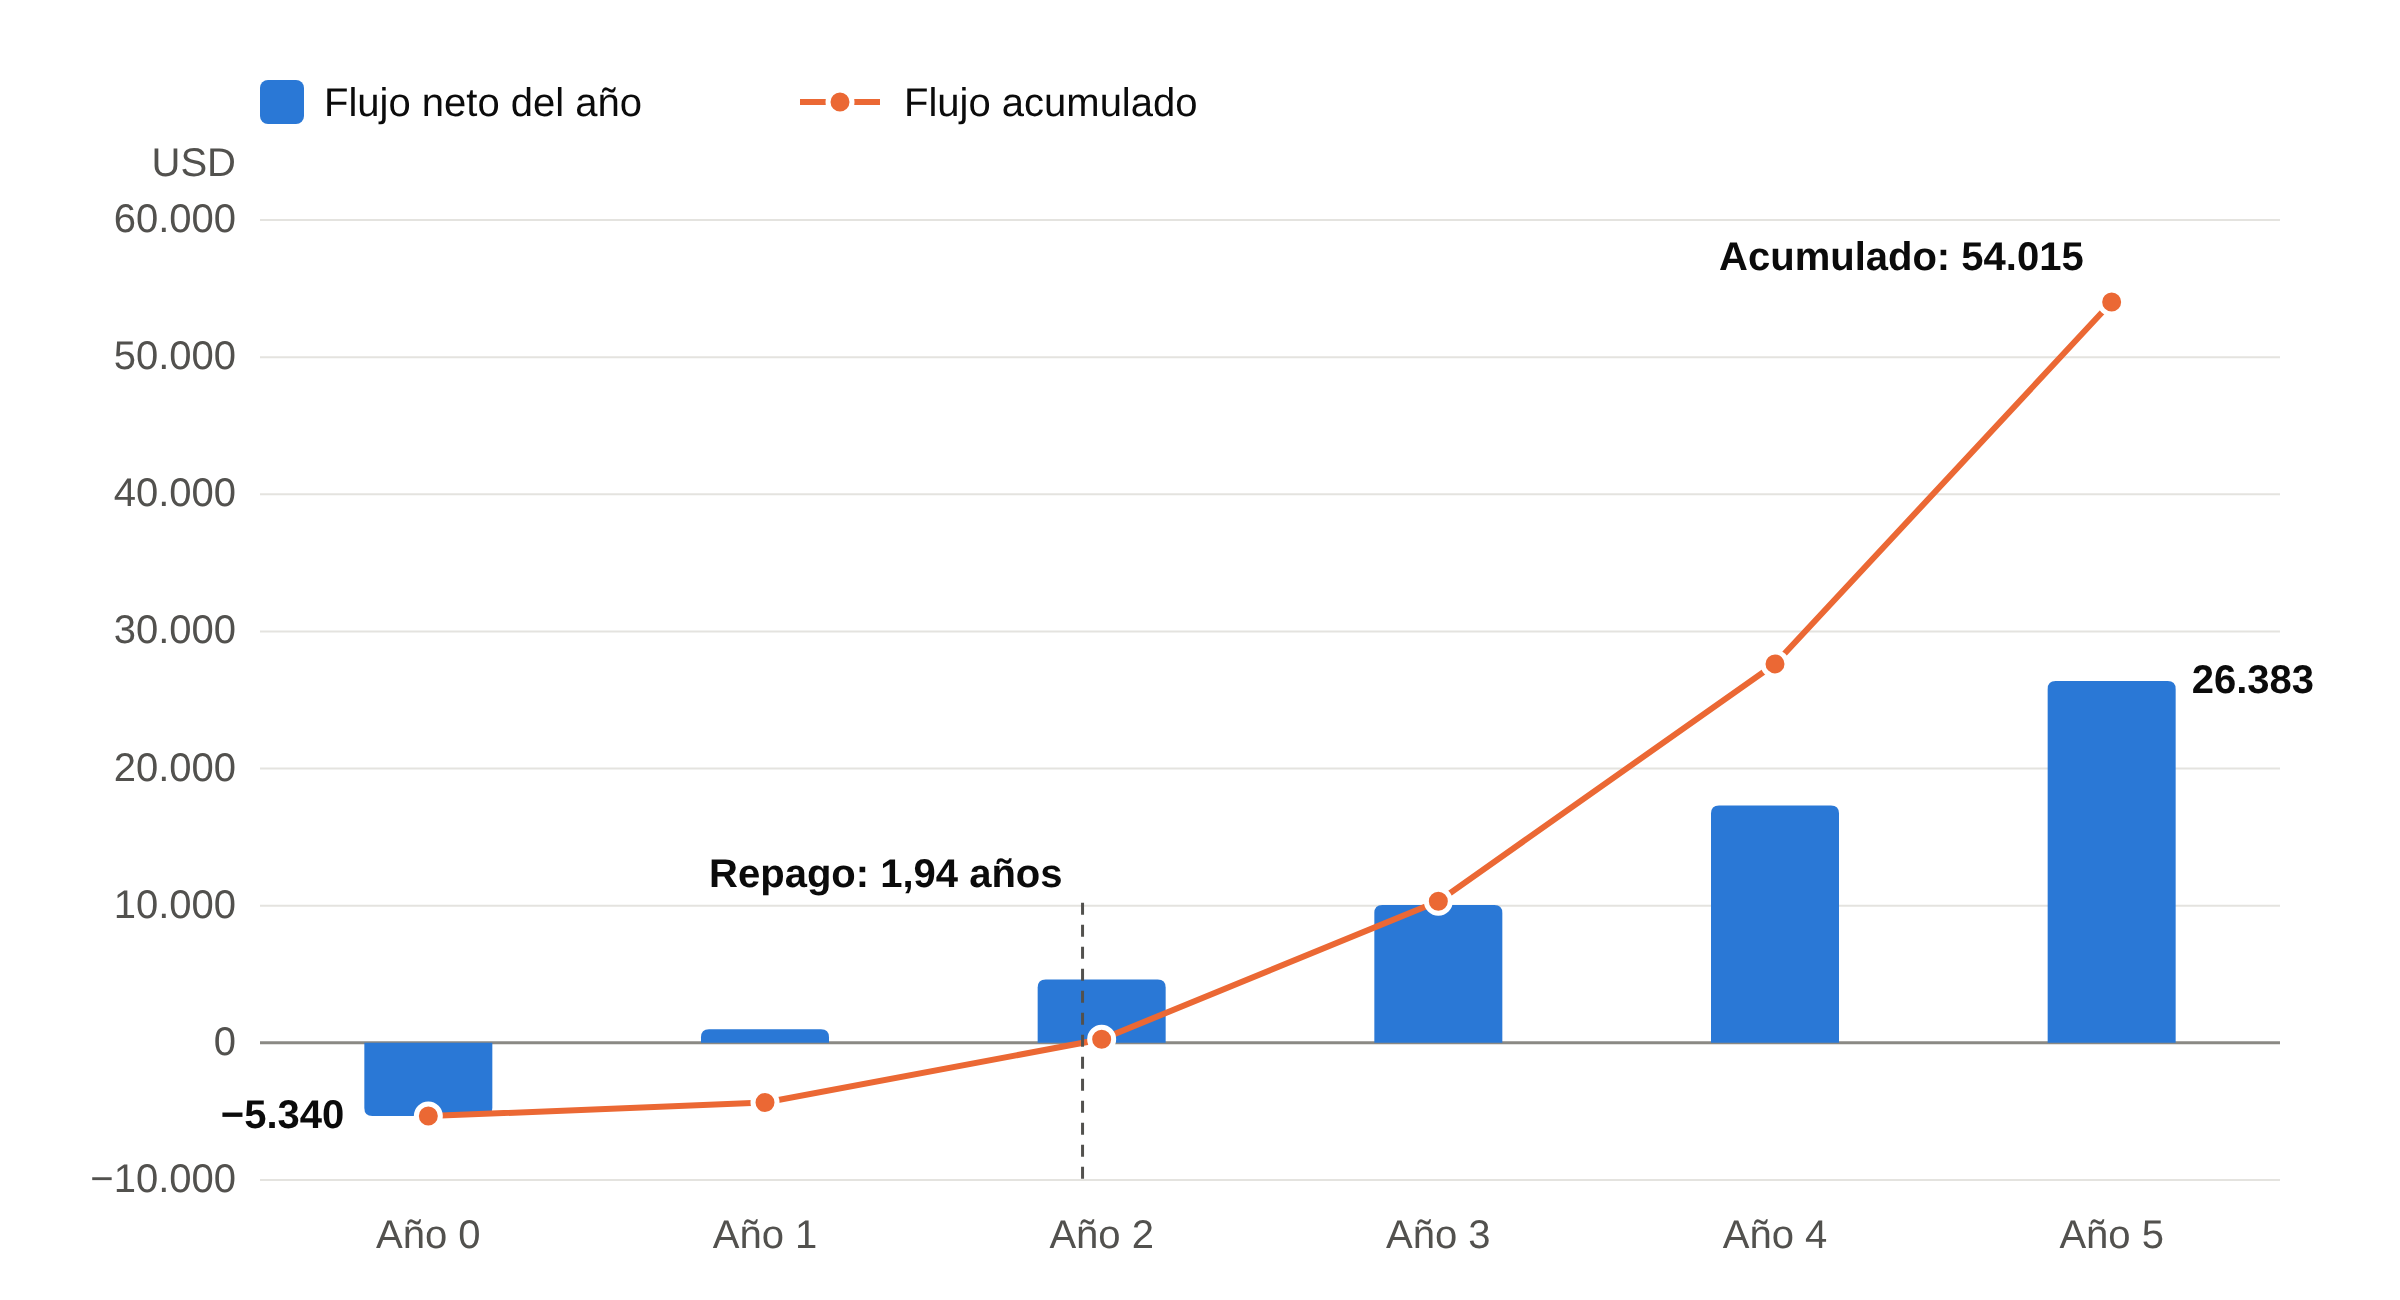
\includegraphics[width=0.9\textwidth]{figuras/flujo-fondos.png}
    \caption{Flujo de fondos neto y acumulado, en dólares (Años 0 a 5). El acumulado se vuelve positivo a los 1,94 años}
    \label{fig:flujo-fondos}
\end{figure}

\section{Tasa de descuento}\label{sec:n5.5}

Se adopta una tasa de descuento del 20 \% anual en dólares. La tasa integra los tres componentes conceptuales del costo de capital.

\paragraph{Costo de oportunidad del capital.} El rendimiento de un activo libre de riesgo en dólares, representado por los bonos del Tesoro de los Estados Unidos a diez años, se ubica en torno al 3,8 \% y el 4,3 \% anual. Una inversión diversificada de mercado en el índice S\&P 500 promedia históricamente un retorno nominal del 9 \% al 10 \% anual en moneda dura.

\paragraph{Inflación de la moneda de evaluación.} Al confeccionar el flujo en dólares se neutraliza la inflación local en pesos, e incide únicamente la meta de inflación de largo plazo del Comité Federal de Mercado Abierto de la Reserva Federal de los Estados Unidos, fijada en el 2 \% anual.

\paragraph{Riesgo específico de etapa temprana.} El proyecto consiste en una herramienta de software que parte sin antecedentes comerciales ni base instalada. La literatura de finanzas corporativas aplicada a la valuación de emprendimientos tecnológicos —en particular las bases de datos de costo de capital de Aswath Damodaran, de la Stern School of Business de la Universidad de Nueva York, y los rangos de referencia empleados para inversiones en etapa semilla— establece tasas de corte de entre el 18 \% y el 25 \% anual en dólares para proyectos tecnológicos incipientes.

Una tasa del 20 \% anual reconoce el costo de oportunidad del capital y remunera de manera adecuada la prima de riesgo asociada a un desarrollo sin tracción comercial previa.

\section{Indicadores financieros}\label{sec:n5.6}

A partir del flujo de fondos de la tabla~\ref{tab:flujo-caja}, y aplicando la tasa de descuento del 20 \%, se obtuvieron los indicadores que expone la tabla~\ref{tab:indicadores-financieros}.

\begin{table}[H]
    \centering
    \caption{Resultados de los indicadores financieros}
    \label{tab:indicadores-financieros}
    \small
    \begin{tabularx}{\textwidth}{l l L l}
        \toprule
        \tb{Indicador} & \tb{Resultado} & \tb{Criterio de decisión} & \tb{Conclusión} \\
        \midrule
        Período de repago simple & 1,94 años & Menor al horizonte de evaluación & Aceptable \\
        Período de repago descontado & 2,23 años & Menor al horizonte de evaluación & Aceptable \\
        Valor Actual Neto (20 \%) & USD 23.459 & VAN > 0 & Crea valor \\
        Tasa Interna de Retorno & 93,5 \% & TIR > 20 \% & Supera el mínimo exigido \\
        \bottomrule
    \end{tabularx}
\end{table}

\subsection{Lectura de los indicadores}\label{sec:n5.6.1}

\paragraph{Repago simple (1,94 años).} El proyecto recupera la inversión inicial durante el segundo año de operación, únicamente con sus flujos netos de caja.

\paragraph{Repago descontado (2,23 años).} Medido en dinero de hoy, el recupero se posterga aproximadamente tres meses y medio respecto del cálculo sin descontar; esa diferencia constituye el precio del tiempo.

\paragraph{Valor Actual Neto (USD 23.459).} El proyecto devuelve la inversión, remunera el 20 \% anual exigido y deja un excedente cercano a los USD 23.500, medidos en dinero de hoy.

\paragraph{Tasa Interna de Retorno (93,5 \%).} El rendimiento anual implícito supera ampliamente la tasa exigida; la tasa de corte podría elevarse hasta ese valor antes de que el proyecto dejara de convenir.

\section{Análisis de sensibilidad y escenarios}\label{sec:n5.7}

\subsection{Sensibilidad del Valor Actual Neto a la tasa de descuento}\label{sec:n5.7.1}

En la tabla~\ref{tab:sensibilidad-tasa} se evalúa la respuesta del Valor Actual Neto ante incrementos sucesivos de la tasa de corte exigida, entre el 10 \% y el 40 \% anual.

\begin{table}[H]
    \centering
    \caption{Sensibilidad del Valor Actual Neto frente a variaciones en la tasa de descuento}
    \label{tab:sensibilidad-tasa}
    \small
    \begin{tabularx}{\textwidth}{l L}
        \toprule
        \tb{Tasa de descuento} & \tb{Valor Actual Neto (USD)} \\
        \midrule
        10 \% & 35.134 \\
        15 \% & 28.636 \\
        20 \% (tasa base) & 23.459 \\
        25 \% & 19.289 \\
        30 \% & 15.895 \\
        40 \% & 10.797 \\
        \bottomrule
    \end{tabularx}
\end{table}

El Valor Actual Neto se mantiene positivo aun elevando la tasa de corte al 40 \%, lo que verifica que la viabilidad del proyecto no depende de una tasa adoptada de forma arbitraria.

\begin{figure}[H]
    \centering
    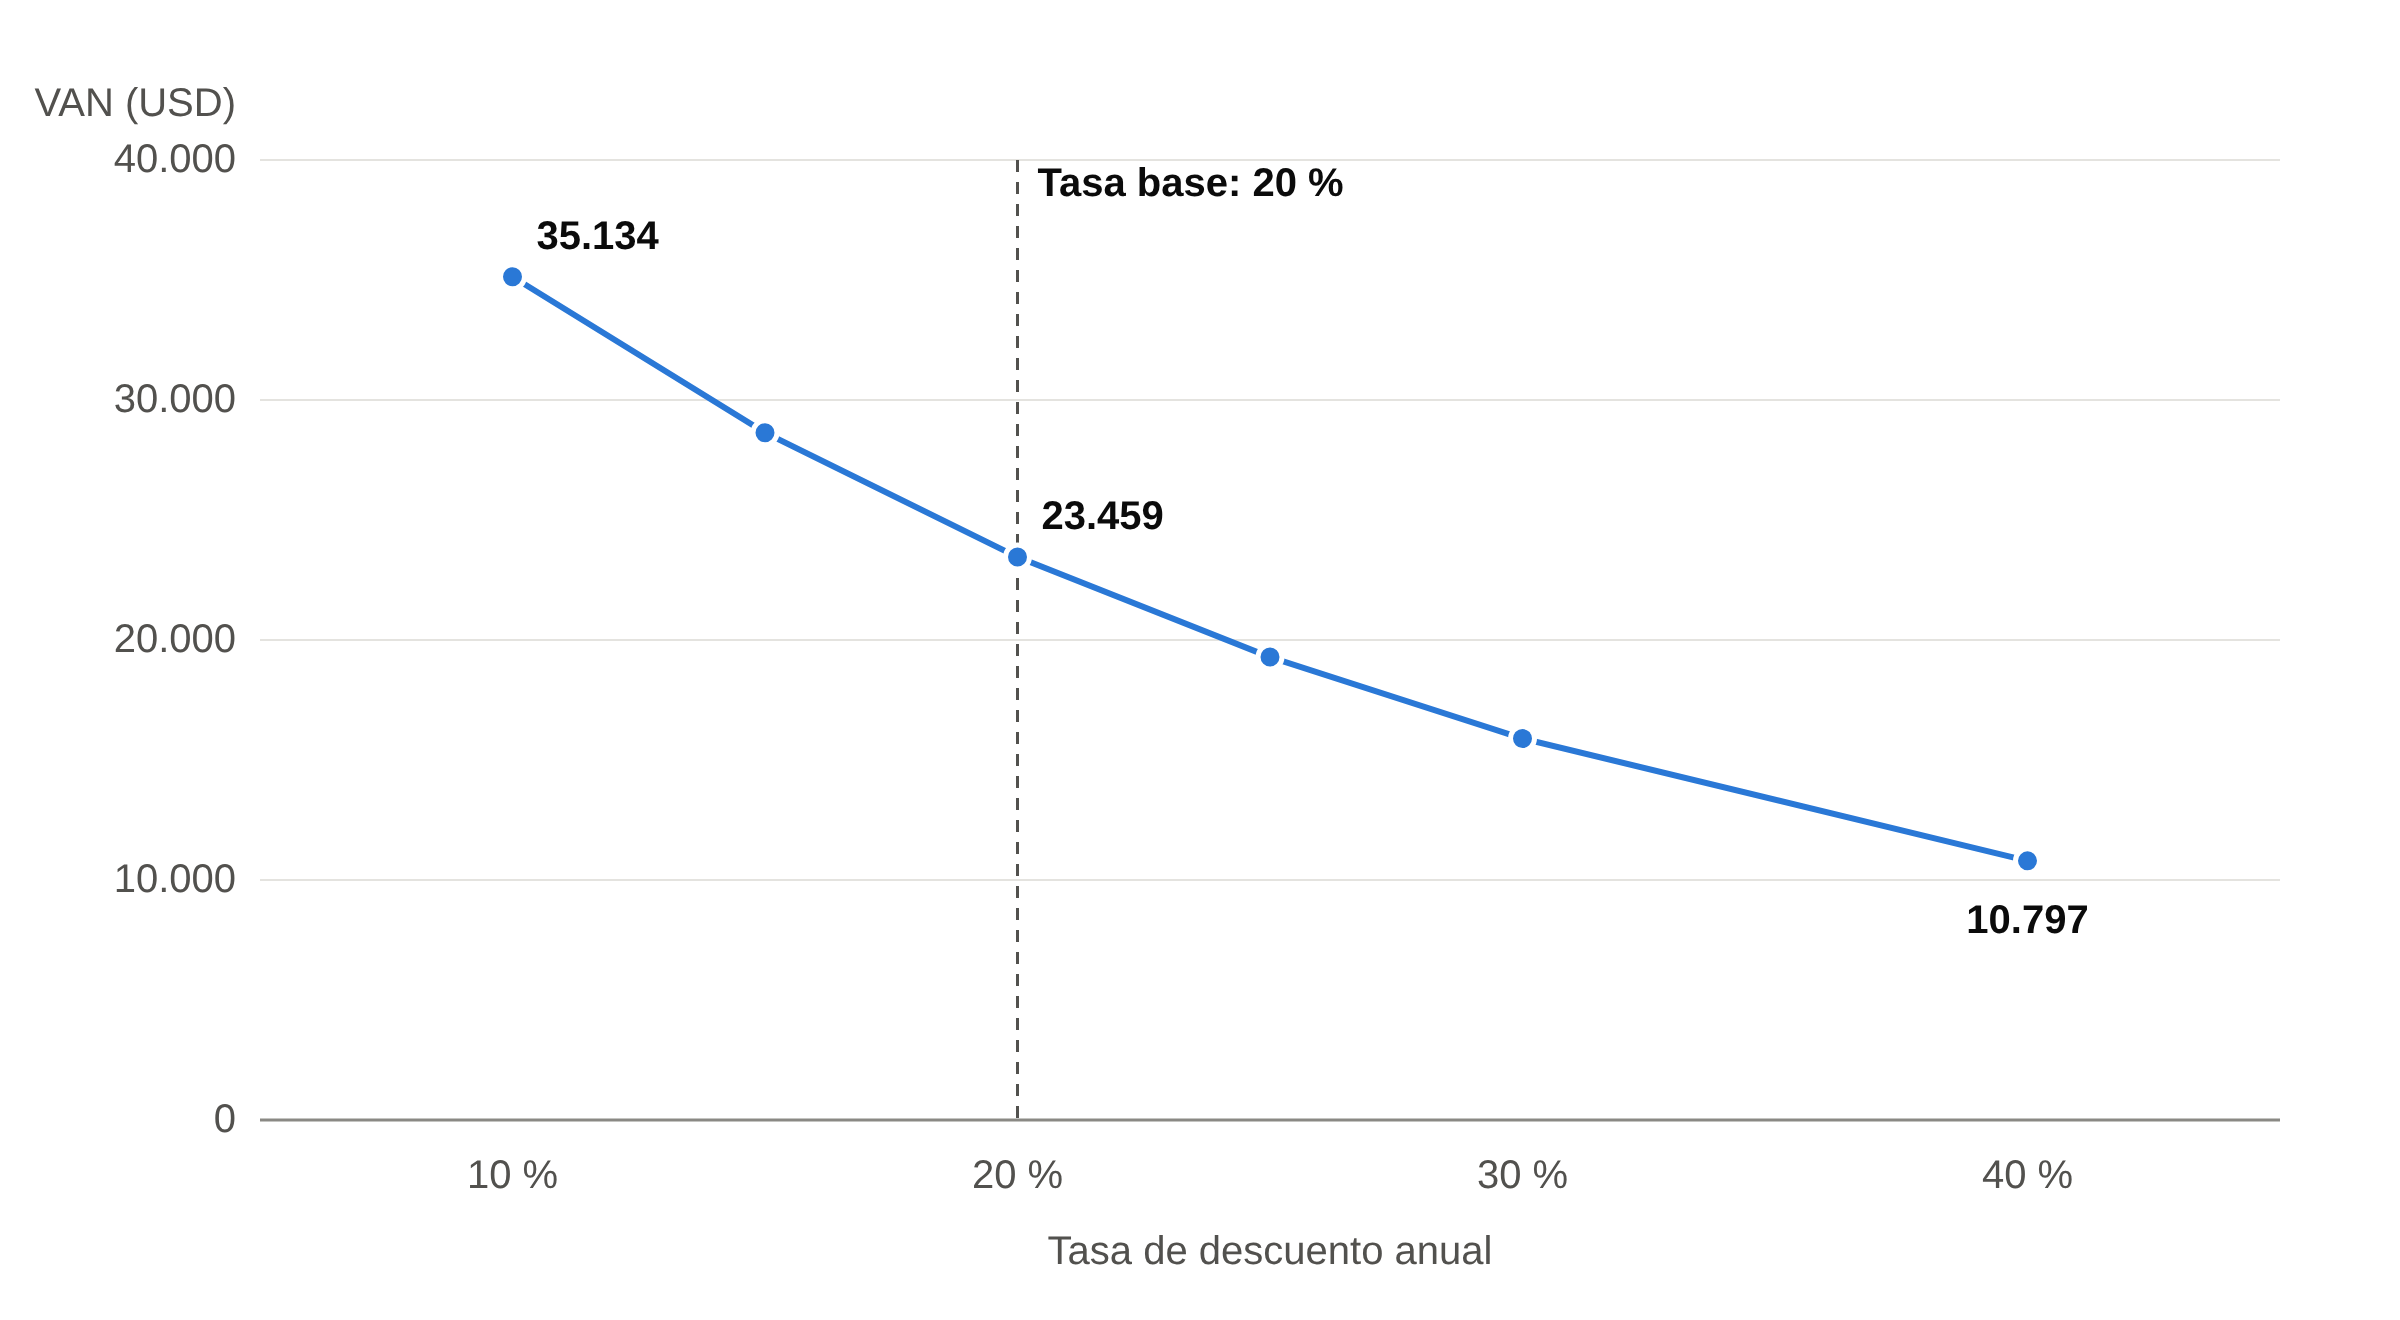
\includegraphics[width=0.9\textwidth]{figuras/van-tasa.png}
    \caption{Valor Actual Neto según la tasa de descuento anual}
    \label{fig:van-tasa}
\end{figure}

\subsection{Escenarios de adopción}\label{sec:n5.7.2}

Siendo la adopción de usuarios la variable de mayor dispersión, la tabla~\ref{tab:escenarios} modela tres situaciones: pesimista, con la mitad de los usuarios proyectados; base, con la proyección original; y optimista, con un 50 \% adicional.

\begin{table}[H]
    \centering
    \caption{Evaluación de escenarios sobre la base de usuarios}
    \label{tab:escenarios}
    \small
    \begin{tabularx}{\textwidth}{l L r r}
        \toprule
        \tb{Escenario} & \tb{Supuesto de usuarios} & \tb{VAN (USD)} & \tb{TIR} \\
        \midrule
        Pesimista & Mitad de los usuarios proyectados (10 a 150) & 7.823 & 51,7 \% \\
        Base & Proyección original adoptada (20 a 300) & 23.459 & 93,5 \% \\
        Optimista & 50 \% adicional sobre la base (30 a 450) & 39.096 & 125,5 \% \\
        \bottomrule
    \end{tabularx}
\end{table}

En el escenario pesimista, captando únicamente la mitad de los usuarios proyectados, el Valor Actual Neto resulta positivo en USD 7.823 y la Tasa Interna de Retorno alcanza el 51,7 \%, superando por 31,7 puntos porcentuales la tasa mínima exigida. El proyecto cuenta, por lo tanto, con margen para absorber desvíos en la captación sin comprometer su conveniencia financiera.

\section{Conclusión}\label{sec:n5.8}

El análisis muestra que el proyecto resulta viable desde el punto de vista económico: los cuatro indicadores calculados señalan rentabilidad positiva dentro del horizonte de cinco años. No obstante, esa viabilidad queda supeditada a condiciones concretas que corresponde declarar.

\subsection{Condición crítica}\label{sec:n5.8.1}

La variable determinante es la captación de usuarios. La inversión de capital es reducida y los costos operativos resultan bajos gracias a que el análisis se ejecuta en el navegador de cada usuario y el servidor solo entrega archivos estáticos. En consecuencia, el riesgo del proyecto no reside en la estructura de costos sino, de manera prácticamente exclusiva, en alcanzar la masa crítica inicial de suscriptores.

\subsection{Magnitud de la Tasa Interna de Retorno}\label{sec:n5.8.2}

El valor obtenido para la Tasa Interna de Retorno responde a la naturaleza económica de los productos de software: una vez cubiertas las horas fijas de desarrollo, el costo marginal de atender a un suscriptor adicional resulta prácticamente nulo. La magnitud del indicador debe interpretarse en ese marco y no como una expectativa de rentabilidad garantizada.

\subsection{Limitaciones del modelo}\label{sec:n5.8.3}

La evaluación incorpora tres simplificaciones que conviene explicitar. En primer lugar, no se incluye una partida continua de costo de adquisición de clientes más allá del gasto de lanzamiento, por asumirse un crecimiento orgánico a través de comunidades técnicas, foros de seguridad y el registro de paquetes npm. En segundo lugar, no se modeló una tasa explícita de deserción: la cantidad de usuarios de cada período se toma como el saldo neto resultante entre altas y cancelaciones. En tercer lugar, se supone facturación anual: si los suscriptores pagaran mes a mes, cada uno generaría doce transacciones y la comisión anual por usuario pasaría de USD 5,30 a USD 10,80, con lo que el Valor Actual Neto descendería a USD 21.563 y la Tasa Interna de Retorno al 89,1 \%; tampoco se incluyeron los cargos adicionales menores que el procesador advierte para algunas transacciones realizadas fuera de Estados Unidos. La incorporación de estos factores reduciría los indicadores obtenidos, si bien el margen que muestra el escenario pesimista sugiere que la conclusión general se mantendría.

\subsection{Conclusión general}\label{sec:n5.8.4}

Bajo la condición de que la efectividad técnica del análisis sustente la recomendación entre desarrolladores y se sostenga la adopción mínima correspondiente al escenario pesimista, el proyecto se justifica económicamente para su ejecución.

    %!TEX root = ../main.tex
% =============================================================
%  CAPÍTULO 6 — ANÁLISIS DE RIESGOS     (Entrega 6 · 5 % · 29/9)
% =============================================================

\chapter{Análisis de riesgos}\label{cap:riesgos}

\begin{guia}[Guía de la cátedra: qué espera ver en este capítulo]
Formato obligatorio de cada riesgo: \textbf{``Debido a [causa], podría
ocurrir [evento], lo que provocaría [efecto]''}. Sin causa es un miedo,
no un riesgo.
\begin{enumerate}
    \item \textbf{Tabla de riesgos} con ID, descripción causa--evento--efecto,
          naturaleza, etapa, probabilidad (1--5), impacto (1--5),
          \gls{exposicion} (1--25), respuesta, responsable y contingencia;
          ordenada por exposición descendente. Con los 6 a 8 primeros bien
          tratados alcanza; el resto se monitorea.
    \item Al menos un riesgo de \textbf{cada naturaleza} (alcance, técnicos,
          recursos, terceros, datos y cumplimiento) y de \textbf{cada etapa}
          (antes de arrancar, durante, pasaje a producción, operación).
    \item Al menos un riesgo \textbf{externo} (``si no tienen ninguno, no
          miraron para afuera'') y al menos uno con respuesta
          \textbf{aceptar} bien justificado (``aceptar se escribe; ignorar
          se paga'').
    \item \textbf{Supuestos y restricciones} separados de los riesgos. Cada
          supuesto que falla se convierte en riesgo.
    \item Que sean propios: ``un riesgo copiado de internet se nota a tres
          metros''.
\end{enumerate}
Los siete que matan proyectos: alcance que nunca cierra (el número uno
de la materia), pérdida de la fuente de datos, equipo que se desarma,
tecnología que no da, inviabilidad de costo, barrera legal o ética,
nadie a cargo. Y la pregunta de jurado: ¿quién lo mantiene cuando
ustedes se reciben? Marco de referencia: \citet{pmi2021}.
\end{guia}

Este capítulo identifica, evalúa y planifica la respuesta a los riesgos del proyecto en su estado actual: un prototipo funcional publicado, con la validación sobre código real y con usuarios todavía en curso, y con cuatro entregas por delante hasta la entrega final del 17 de noviembre. Reemplaza y amplía la tabla~\ref{tab:riesgos-iniciales} del capítulo~\ref{cap:metodologia}, que registraba tres riesgos técnicos identificados durante la planificación. Varios de los riesgos que se presentan no son hipotéticos: surgieron durante el desarrollo, y en esos casos se indica la evidencia que los originó.

\section{Enfoque y escalas de evaluación}\label{sec:n6.1}

El marco de referencia es la guía del \citet{pmi2021}, que trata el riesgo como un evento o una condición incierta que, si ocurre, afecta al menos uno de los objetivos del proyecto. Cada riesgo se redacta con una estructura de causa, evento y efecto: «Debido a [causa], podría ocurrir [evento], lo que provocaría [efecto]». La causa es la condición presente que lo origina y sobre la que se puede actuar; el evento, lo que podría suceder; y el efecto, su consecuencia sobre los objetivos.

La probabilidad (P) y el impacto (I) se califican en una escala de 1 a 5, y la exposición (E) se obtiene como su producto, con valores entre 1 y 25. La tabla~\ref{tab:exposicion} fija los niveles de exposición: baja hasta 5, media entre 6 y 10, y alta desde 12.

\paragraph{Probabilidad.} 1 muy improbable; 2 poco probable; 3 posible; 4 probable; 5 muy probable.

\paragraph{Impacto.} 1 insignificante, sin efecto visible en los entregables; 2 menor, un retrabajo acotado dentro de la misma semana; 3 moderado, afecta la calidad de un entregable sin comprometer su fecha; 4 importante, compromete una entrega o una hipótesis; 5 severo, compromete la aprobación del proyecto o la defensa.

\begin{table}[H]
    \centering
    \caption{Matriz de exposición: probabilidad por impacto}
    \label{tab:exposicion}
    \small
    \begin{tabular}{l c c c c c}
        \toprule
        \tb{Probabilidad / Impacto} & \tb{1 Insignif.} & \tb{2 Menor} & \tb{3 Moderado} & \tb{4 Importante} & \tb{5 Severo} \\
        \midrule
        \tb{5 Muy probable} & \riesgoBajo{5} & \riesgoMedio{10} & \riesgoAlto{15} & \riesgoAlto{20} & \riesgoAlto{25} \\
        \tb{4 Probable} & \riesgoBajo{4} & \riesgoMedio{8} & \riesgoAlto{12} & \riesgoAlto{16} & \riesgoAlto{20} \\
        \tb{3 Posible} & \riesgoBajo{3} & \riesgoMedio{6} & \riesgoMedio{9} & \riesgoAlto{12} & \riesgoAlto{15} \\
        \tb{2 Poco probable} & \riesgoBajo{2} & \riesgoBajo{4} & \riesgoMedio{6} & \riesgoMedio{8} & \riesgoMedio{10} \\
        \tb{1 Muy improbable} & \riesgoBajo{1} & \riesgoBajo{2} & \riesgoBajo{3} & \riesgoBajo{4} & \riesgoBajo{5} \\
        \bottomrule
    \end{tabular}
\end{table}

Para cada riesgo se elige una de cuatro respuestas: evitar, que elimina la causa, por ejemplo modificando el alcance; mitigar, que reduce la probabilidad o el impacto; transferir, que traslada el riesgo a un tercero con mayor capacidad de absorberlo; y aceptar, que convive con el riesgo en forma documentada, con un responsable y un plan de contingencia. Los riesgos se clasifican además por su naturaleza (alcance, técnica, recursos, terceros, datos y cumplimiento), por la etapa en la que pueden materializarse (antes de arrancar, durante el desarrollo, en el pasaje a producción y durante la operación) y según su origen sea interno o externo al proyecto.

\section{Supuestos y restricciones}\label{sec:n6.2}

Los supuestos son condiciones que se dan por ciertas sin haberlas verificado; las restricciones, límites que el proyecto no puede modificar. Se registran por separado porque no son riesgos, aunque cada supuesto que deja de cumplirse se convierte en uno. La tabla~\ref{tab:supuestos-restricciones} indica con qué riesgo o sección se vincula cada uno.

\begin{table}[H]
    \centering
    \caption{Supuestos (S) y restricciones (C) del proyecto}
    \label{tab:supuestos-restricciones}
    \small
    \begin{tabularx}{\textwidth}{l L l}
        \toprule
        \tb{ID} & \tb{Supuesto o restricción} & \tb{Vínculo} \\
        \midrule
        S-01 & Los usuarios de la versión web cuentan con un navegador actualizado, con soporte para Web Workers y módulos ES. & R-12 \\
        S-02 & Las operaciones sensibles que emplean las aplicaciones analizadas coinciden con las registradas en el catálogo: consultas SQL, ejecución de procesos, escritura en el documento y métodos de Mongoose. & R-01, R-08 \\
        S-03 & Existen aplicaciones Node.js deliberadamente vulnerables, con vulnerabilidades documentadas y una licencia que permite analizarlas, como OWASP NodeGoat (licencia Apache-2.0). & R-02 \\
        S-04 & Se consiguen entre cinco y ocho desarrolladores dispuestos a participar de la validación de la hipótesis H3 entre el 5 y el 9 de octubre. & R-06 \\
        S-05 & Vercel mantiene las condiciones y el precio del plan Pro (USD 20 mensuales) durante el horizonte de evaluación. & Capítulo 5 (Tabla 14) \\
        S-06 & El procesador de pagos admite vendedores radicados en Argentina y mantiene su comisión del 5 \% más USD 0,50 por transacción. & Capítulo 5 (Tabla 14) \\
        C-01 & Restricción: el proyecto tiene un único integrante, con una dedicación parcial de tres a cuatro días por semana. & R-11 \\
        C-02 & Restricción: las fechas son fijas; capítulo 7 el 13 de octubre, capítulo 8 el 20 de octubre, documento integrado el 27 de octubre, sistema congelado el 3 de noviembre y entrega final el 17 de noviembre. & R-03 \\
        C-03 & Restricción: durante el desarrollo no hay presupuesto; se emplean herramientas libres y planes gratuitos. & R-09 \\
        C-04 & Restricción: el código analizado no puede salir del equipo del usuario, por lo que el análisis se ejecuta en el navegador o en la interfaz de línea de comandos, sin procesamiento en un servidor. & R-12 \\
        C-05 & Restricción: el alcance se limita a JavaScript y TypeScript y a las cuatro familias de debilidades del catálogo. & R-01 \\
        \bottomrule
    \end{tabularx}
\end{table}

\section{Matriz de riesgos}\label{sec:n6.3}

La tabla~\ref{tab:matriz-riesgos} registra los doce riesgos identificados, ordenados por exposición descendente. Cubren las seis naturalezas y las cuatro etapas; tres son de origen externo (R-06, R-07 y R-09) y uno se acepta en forma explícita (R-11). Los ocho primeros, de exposición alta, se desarrollan en la sección~\ref{sec:n6.4}; los restantes se revisan según lo indicado en la sección~\ref{sec:n6.7}.

\begin{landscape}
\footnotesize
\begin{xltabular}{\linewidth}{l >{\hsize=1.5\hsize}L >{\raggedright\arraybackslash}p{1.9cm} >{\raggedright\arraybackslash}p{1.6cm} c c c >{\hsize=0.9\hsize}L p{0.9cm} >{\hsize=0.6\hsize}L}
    \caption{Matriz de riesgos ordenada por exposición. P: probabilidad; I: impacto; E: exposición}
    \label{tab:matriz-riesgos} \\
    \toprule
    \tb{ID} & \tb{Descripción (causa, evento, efecto)} & \tb{Naturaleza} & \tb{Etapa} & \tb{P} & \tb{I} & \tb{E} & \tb{Respuesta} & \tb{Resp.} & \tb{Contingencia} \\
    \midrule
    \endfirsthead
    \toprule
    \tb{ID} & \tb{Descripción (causa, evento, efecto)} & \tb{Naturaleza} & \tb{Etapa} & \tb{P} & \tb{I} & \tb{E} & \tb{Respuesta} & \tb{Resp.} & \tb{Contingencia} \\
    \midrule
    \endhead
    \bottomrule
    \endfoot
    R-01 & Debido a que el motor solo resuelve llamadas a funciones declaradas con function e importadas mediante módulos ES, podría ocurrir que en aplicaciones Express escritas con funciones flecha, clases o require el analizador no siga el recorrido del dato, lo que provocaría una exhaustividad baja sobre código real y dejaría sin sustento a la hipótesis H1 fuera del banco sintético. & Técnica & Durante & 4 & 5 & \riesgoAlto{20} & Mitigar: incorporar al alcance congelado solo las funciones flecha asignadas a constantes y los callbacks de rutas de Express; declarar el resto como limitación. & Autor & Presentar H1 como validada sobre el subconjunto soportado, con la exhaustividad desglosada por construcción. \\
    R-02 & Debido a que los advisories de npm corresponden mayormente a bibliotecas publicadas como código compilado o con fallas en su propia lógica de filtrado, podría ocurrir que el corpus de vulnerabilidades reales no tenga casos evaluables por el modelo de origen y destino, lo que provocaría no poder medir el desempeño sobre código real. & Datos & Durante & 5 & 4 & \riesgoAlto{20} & Mitigar: sumar aplicaciones deliberadamente vulnerables con vulnerabilidades documentadas, como OWASP NodeGoat, etiquetadas antes de analizarlas. & Autor & Declarar la validación sobre código real como preliminar en los capítulos 7 y 8. \\
    R-03 & Debido a que cada construcción no soportada que aparece en un caso de prueba se percibe como una mejora pendiente del motor, podría ocurrir que el alcance técnico siga creciendo después del congelamiento, lo que provocaría llegar a la defensa con funciones incompletas y sin tiempo para integrar el documento. & Alcance & Durante & 4 & 4 & \riesgoAlto{16} & Evitar: cerrar la lista de mejoras el 13 de octubre; lo posterior pasa a trabajo futuro. & Autor & Volver a la última versión etiquetada estable. \\
    R-04 & Debido a que los destinos sensibles se reconocen por el nombre de la función invocada, podría ocurrir que llamadas homónimas sin relación con el riesgo se reporten como vulnerabilidades, lo que provocaría falsos positivos que contradicen la propuesta de valor del sistema. & Técnica & Operación & 4 & 3 & \riesgoAlto{12} & Mitigar: calificar los destinos por el objeto receptor o el módulo importado, por ejemplo exec de child\_process. & Autor & Documentar las reglas afectadas como de baja confianza. \\
    R-05 & Debido a que las dependencias del proyecto registran vulnerabilidades conocidas, podría ocurrir que el jurado o un usuario las detecte en el repositorio, lo que provocaría una pérdida de credibilidad especialmente grave para una herramienta de seguridad. & Cumplimiento & Pasaje a producción & 4 & 3 & \riesgoAlto{12} & Mitigar: revisar las alertas, actualizar las dependencias y fijar sus versiones antes del 3 de noviembre. & Autor & Documentar en el README las alertas pendientes y su impacto real. \\
    R-06 & Debido a que la validación de H3 depende de desarrolladores externos que participan en forma voluntaria, podría ocurrir que no se reúnan participantes suficientes en la semana prevista, lo que provocaría no poder contrastar la hipótesis sobre la visualización. & Terceros (externo) & Durante & 3 & 4 & \riesgoAlto{12} & Mitigar: convocatoria anticipada, sesiones remotas de veinte minutos y un protocolo breve. & Autor & Estudio reducido declarado preliminar, complementado con la entrevista a un experto. \\
    R-07 & Debido a que existen herramientas consolidadas con análisis de flujo de datos, como Semgrep y CodeQL, gratuitas en determinadas condiciones de uso, podría ocurrir que los desarrolladores no estén dispuestos a pagar una suscripción, lo que provocaría una captación inferior a la proyectada en el capítulo 5. & Recursos (externo) & Operación & 3 & 4 & \riesgoAlto{12} & Mitigar: posicionar el producto por el análisis desde el navegador sin instalación y por la visualización del recorrido, y relevar la disposición a pagar en la validación con usuarios. & Autor & Reformular el modelo hacia un esquema gratuito con funciones pagas. \\
    R-08 & Debido a que el catálogo de orígenes, destinos y sanitizadores depende de APIs de bibliotecas que evolucionan y el autor es su único mantenedor, podría ocurrir que después de la entrega el catálogo quede desactualizado, lo que provocaría falsos negativos crecientes. & Datos & Operación & 4 & 3 & \riesgoAlto{12} & Transferir: publicar el código con licencia abierta y documentar cómo extender el catálogo en JSON para recibir contribuciones. & Autor & Indicar en el README la fecha de la última revisión del catálogo. \\
    R-09 & Debido a que la versión publicada depende de Vercel y de la conectividad del aula, podría ocurrir que el sitio no esté disponible durante la defensa, lo que impediría mostrar el sistema funcionando al jurado. & Terceros (externo) & Pasaje a producción & 2 & 5 & \riesgoMedio{10} & Mitigar: ejecución local preparada y video de la demostración grabado la semana anterior. & Autor & Mostrar el video y ejecutar la versión local. \\
    R-10 & Debido a que el repositorio no declara una licencia, podría ocurrir que el código no pueda reutilizarse ni mantenerse legalmente por terceros, lo que provocaría la falta de continuidad del proyecto e incumpliría un requisito de la cátedra. & Cumplimiento & Antes de arrancar & 5 & 2 & \riesgoMedio{10} & Evitar: agregar una licencia MIT, compatible con las licencias MIT y Apache-2.0 de las dependencias principales. & Autor & No aplica: la respuesta elimina la causa. \\
    R-11 & Debido a que el proyecto tiene un único integrante con dedicación parcial, podría ocurrir una enfermedad o una sobrecarga en las semanas previas a la entrega, lo que provocaría atrasos en las entregas 7 y 8. & Recursos & Durante & 2 & 4 & \riesgoMedio{8} & Aceptar: no hay reemplazo posible; el margen de cuatro semanas entre la entrega 8 y la final absorbe una semana de atraso, y el avance queda versionado. & Autor & Priorizar el documento sobre nuevas funciones y solicitar una prórroga con evidencia. \\
    R-12 & Debido a que el análisis se ejecuta en el navegador con el compilador de TypeScript, un módulo de unos 5,9 MB, y mantiene en memoria el grafo del proyecto, podría ocurrir que en proyectos grandes o en equipos modestos el análisis tarde demasiado o agote la memoria de la pestaña, lo que provocaría que el usuario no obtenga resultados. & Técnica & Operación & 2 & 3 & \riesgoMedio{6} & Mitigar: excluir dependencias y archivos de más de 1 MB, mostrar el progreso y ofrecer la interfaz de línea de comandos para proyectos grandes. & Autor & Analizar el proyecto con la interfaz de línea de comandos. \\
\end{xltabular}
\end{landscape}

\section{Tratamiento de los riesgos principales}\label{sec:n6.4}

Los ocho riesgos de exposición alta se desarrollan con la evidencia que los sostiene, la respuesta planificada y el indicador con el que se controla su evolución.

\subsection{R-01: alcance del motor frente a aplicaciones reales}\label{sec:n6.4.1}

\paragraph{Evidencia.} La resolución de llamadas se limita a funciones declaradas por nombre (sección~\ref{sec:n4.2.5}). Sobre el código del propio sistema, el enlace entre archivos resolvió 369 llamadas en 78 archivos, pero los callbacks de rutas de Express y los métodos de clase quedan fuera del recorrido.

\paragraph{Respuesta.} Se incorporan al alcance congelado únicamente las funciones flecha asignadas a constantes y los callbacks de rutas de Express, dos formas habituales en las aplicaciones objetivo; el resto de las construcciones se declara como limitación.

\paragraph{Seguimiento.} Exhaustividad sobre el corpus de aplicaciones reales, desglosada por construcción sintáctica. Si al 13 de octubre se mantiene por debajo del 50 \%, se aplica la contingencia.

\subsection{R-02: corpus de vulnerabilidades reales}\label{sec:n6.4.2}

\paragraph{Evidencia.} En la validación del capítulo~\ref{cap:marco-tecnologico} (tabla~\ref{tab:advisories}), tres de los seis advisories no tenían código fuente analizable en el paquete publicado, y en los restantes la falla residía en la lógica interna de bibliotecas de saneamiento. El riesgo ya se materializó en forma parcial.

\paragraph{Respuesta.} Se suma OWASP NodeGoat, una aplicación Node.js construida con fines didácticos para mostrar los riesgos del OWASP Top 10 y distribuida con licencia Apache-2.0. Antes de ejecutar el analizador se etiquetan las vulnerabilidades documentadas que corresponden al catálogo, para que la medición no se ajuste a los resultados.

\paragraph{Seguimiento.} Cantidad de casos etiquetados y evaluables al 6 de octubre.

\subsection{R-03: alcance que no cierra}\label{sec:n6.4.3}

\paragraph{Evidencia.} Durante el desarrollo se sumaron el análisis entre archivos, la versión web y una cuarta familia de debilidades (CWE-943), ninguno de ellos previsto en el alcance definido en el capítulo~\ref{cap:metodologia}.

\paragraph{Respuesta.} El 13 de octubre se cierra la lista de mejoras del motor. Toda mejora posterior se registra como trabajo futuro en el capítulo~\ref{cap:conclusiones}, y desde el 3 de noviembre el repositorio solo admite correcciones de errores.

\paragraph{Seguimiento.} Cada entrega se etiqueta en el repositorio, desde entrega-6 hasta entrega-final, lo que permite comparar el alcance entregado con el comprometido.

\subsection{R-04: falsos positivos por coincidencia de nombres}\label{sec:n6.4.4}

\paragraph{Evidencia.} Al analizar el código del propio sistema, una llamada a \texttt{RegExp.\allowbreak prototype.\allowbreak exec} se reportó como inyección de comandos (CWE-78), porque coincide por nombre con el destino exec del catálogo.

\paragraph{Respuesta.} Se califica cada destino por el objeto receptor o por el módulo del que se importa la función, de modo que exec solo se considere sensible cuando proviene de child\_process.

\paragraph{Seguimiento.} Falsos positivos del banco sintético, hoy nulos, y del corpus de aplicaciones reales.

\subsection{R-05: dependencias con vulnerabilidades conocidas}\label{sec:n6.4.5}

\paragraph{Evidencia.} Al publicar la rama principal, GitHub informó doce alertas de dependencias, tres de ellas críticas, y la instalación en Vercel reportó ocho vulnerabilidades en el árbol de dependencias.

\paragraph{Respuesta.} Antes del congelamiento se revisa cada alerta, se actualizan las dependencias afectadas y se distingue entre las que llegan a la versión publicada y las que solo intervienen en el desarrollo.

\paragraph{Seguimiento.} Cantidad de alertas críticas y altas abiertas en el repositorio; el objetivo es no tener ninguna al 3 de noviembre.

\subsection{R-06: participantes para la validación de H3}\label{sec:n6.4.6}

\paragraph{Evidencia.} La hipótesis H3 compara la interpretación del riesgo con y sin visualización, algo que el banco de pruebas no puede medir y que depende de personas externas al proyecto.

\paragraph{Respuesta.} La convocatoria se realiza con dos semanas de anticipación, con sesiones remotas de veinte minutos: cada participante localiza el camino vulnerable en un reporte de texto y en el grafo, y se registran el tiempo, el acierto y una valoración en escala de Likert.

\paragraph{Seguimiento.} Participantes confirmados al 1 de octubre; con menos de cinco se aplica la contingencia.

\subsection{R-07: competencia de herramientas gratuitas}\label{sec:n6.4.7}

\paragraph{Evidencia.} Semgrep y CodeQL implementan análisis de flujo de datos (capítulo~\ref{cap:marco-teorico}) y se ofrecen sin costo en determinadas condiciones de uso. El capítulo~\ref{cap:economica} identificó la captación de usuarios como la condición crítica de la viabilidad económica.

\paragraph{Respuesta.} El producto se posiciona por el análisis desde el navegador, sin instalación y sin envío del código, y por la visualización interactiva del recorrido del dato. La validación con usuarios incorpora una pregunta sobre la disposición a pagar.

\paragraph{Seguimiento.} Resultados de esa pregunta; si la mayoría de los participantes rechaza el precio, se revisa el escenario del capítulo~\ref{cap:economica}.

\subsection{R-08: mantenimiento del catálogo}\label{sec:n6.4.8}

\paragraph{Evidencia.} El catálogo registra 23 destinos sensibles y 18 sanitizadores en cuatro archivos JSON, y cada nueva versión de una biblioteca puede introducir operaciones que no figuran en él.

\paragraph{Respuesta.} Se publica el código con licencia abierta (R-10) y se documenta en el README cómo agregar una entrada al catálogo, para que otros desarrolladores puedan contribuir. La sección~\ref{sec:n6.6} desarrolla la continuidad del sistema.

\paragraph{Seguimiento.} Fecha de la última revisión del catálogo, registrada en el historial del repositorio.

\section{Riesgos críticos de un proyecto final}\label{sec:n6.5}

La cátedra identifica siete riesgos que con mayor frecuencia hacen fracasar un proyecto final. La tabla~\ref{tab:riesgos-criticos} indica cómo se presenta cada uno en este proyecto y dónde se trata.

\begin{table}[H]
    \centering
    \caption{Relación entre los riesgos críticos de un proyecto final y los riesgos identificados}
    \label{tab:riesgos-criticos}
    \small
    \begin{tabularx}{\textwidth}{L L l}
        \toprule
        \tb{Riesgo crítico} & \tb{Cómo se presenta en este proyecto} & \tb{Tratamiento} \\
        \midrule
        Alcance que nunca cierra & El motor admite mejoras indefinidas: cada construcción del lenguaje no soportada es una candidata. & R-03 \\
        Pérdida de la fuente de datos & El corpus de vulnerabilidades reales resultó poco evaluable. & R-02 \\
        Equipo que se desarma & El equipo es de una persona y no tiene reemplazo. & R-11 \\
        Tecnología que no da & La resolución de llamadas limita el desempeño sobre código real, y el navegador limita el tamaño de proyecto analizable. & R-01, R-12 \\
        Inviabilidad de costo & El costo de desarrollo es nulo; en la operación, la viabilidad depende de la captación y no de los costos (capítulo 5). & R-07 \\
        Barrera legal o ética & El código analizado no sale del equipo del usuario, lo que evita tratar código de terceros en servidores propios; falta declarar la licencia del repositorio. & R-10 \\
        Nadie a cargo & El autor es el único responsable del mantenimiento después de la entrega. & R-08 \\
        \bottomrule
    \end{tabularx}
\end{table}

\section{Continuidad del sistema después de la entrega}\label{sec:n6.6}

La pregunta sobre quién mantiene el sistema cuando el autor se recibe se responde con tres decisiones. Primero, el código se publicará con licencia MIT en un repositorio público (R-10), lo que permite que cualquier persona lo use, lo modifique y lo continúe. Segundo, la parte que más cambia con el tiempo, las reglas de detección, está separada del motor en los archivos JSON del catálogo, de modo que actualizarla no requiere conocer la implementación del análisis. Tercero, la versión web no tiene componentes de servidor ni base de datos que administrar: el despliegue en Vercel se reconstruye a partir del repositorio, y mantenerla en línea para uso no comercial no tiene costo.

El autor asume el mantenimiento durante el horizonte de evaluación del capítulo~\ref{cap:economica}. Si el proyecto no continúa como producto, queda disponible como herramienta académica de código abierto.

\section{Seguimiento y actualización}\label{sec:n6.7}

La matriz se revisa en cada entrega, al etiquetar la versión correspondiente en el repositorio: se actualizan la probabilidad y el impacto de cada riesgo, se registran los que se materializaron y se agregan los nuevos. Los riesgos R-09 a R-12 no tienen un tratamiento desarrollado más allá de la respuesta de la tabla~\ref{tab:matriz-riesgos} y se revisan en esas mismas instancias.

Las fechas de control son el 1 de octubre para la convocatoria de participantes (R-06), el 6 de octubre para el corpus de aplicaciones reales (R-02), el 13 de octubre para el cierre del alcance (R-03) y el 3 de noviembre para las dependencias y la licencia (R-05 y R-10).

    %!TEX root = ../main.tex
% =============================================================
%  CAPÍTULO 7 — PRESENTACIÓN DE RESULTADOS
%                                       (Entrega 7 · 5 % · 13/10)
% =============================================================

\chapter{Presentación de resultados}\label{cap:resultados}

\begin{guia}[Guía de la cátedra: qué se evalúa en este capítulo]
\begin{enumerate}
    \item \textbf{Requerimientos formales}: \gls{rf} y \gls{rnf} con ID,
          descripción, prioridad y criterio de aceptación medible,
          trazados a los indicadores del capítulo~\ref{cap:metodologia}.
    \item \textbf{Evidencia de implementación}: capturas reales del sistema
          funcionando, enlaces al repositorio (anexo~\ref{anx:repositorios})
          y al despliegue.
    \item \textbf{Resultados cuantitativos honestos}: diseño experimental,
          métricas, matrices de confusión o su equivalente en el dominio,
          incluyendo lo que salió mal y su análisis. Reportar también lo
          malo y argumentarlo vale más que esconderlo. Hiperparámetros y
          versiones en el apéndice~\ref{apx:tecnicos}.
    \item \textbf{Validación con usuarios y expertos}: idealmente
          triangulada (métricas técnicas, encuesta, entrevista) y
          traducida a decisiones de diseño concretas. Instrumentos en los
          apéndices \ref{apx:encuesta} y \ref{apx:entrevista}.
\end{enumerate}
El sistema tiene que existir y andar: la entrega final incluye el
proyecto funcional.
\end{guia}

Este capítulo presenta la evidencia obtenida durante el desarrollo y la
validación de GraphSAST. Se organiza en cinco partes: los requerimientos
que el sistema debía cumplir, el proceso con el que se construyó, la
evidencia de que funciona, los resultados de las pruebas técnicas y los
de la validación con usuarios. Se informan tanto los resultados
favorables como los desfavorables, y la lectura de cada hipótesis se
reserva para el capítulo~\ref{cap:conclusiones}.

Los objetivos específicos del capítulo~\ref{cap:introduccion} se
identifican en adelante como OE-1 a OE-6, en el orden en que allí se
enuncian: analizador sintáctico (OE-1), construcción del grafo (OE-2),
motor de contaminación (OE-3), persistencia en Neo4j (OE-4), interfaz de
visualización (OE-5) y validación (OE-6).

% -------------------------------------------------------------
\section{Requerimientos del sistema}\label{sec:requerimientos}
% -------------------------------------------------------------

Los requerimientos se derivan de los objetivos específicos y de los
indicadores de evaluación definidos en el capítulo~\ref{cap:metodologia}
(tabla~\ref{tab:indicadores}). Cada requerimiento funcional indica el
objetivo al que responde y un criterio de aceptación verificable sobre
el sistema construido; la verificación de cada criterio se presenta en
la sección~\ref{sec:pruebas}.

\begin{table}[H]
    \centering
    \caption{Requerimientos funcionales}
    \label{tab:rf}
    \footnotesize
    \begin{tabularx}{\textwidth}{@{}l >{\hsize=.75\hsize}L >{\hsize=1.25\hsize}L l l L@{}}
        \toprule
        \tb{ID} & \tb{Nombre} & \tb{Descripción} & \tb{Prior.} & \tb{Obj.} & \tb{Criterio de aceptación} \\
        \midrule
        RF-01 & Análisis sintáctico & Obtener el árbol de sintaxis abstracta de archivos TypeScript y JavaScript & Alta & OE-1 & Los 43 casos del banco sintético se analizan sin errores \\
        RF-02 & Construcción del grafo & Generar los cinco tipos de nodo y las cinco relaciones del modelo & Alta & OE-2 & Pasan todas las pruebas de representación intermedia y flujo de datos \\
        RF-03 & Detección de caminos & Reportar caminos de un origen a un destino sensible sin saneamiento, según el catálogo JSON & Alta & OE-3 & Se detectan los 29 casos vulnerables del banco sintético \\
        RF-04 & Descarte de saneados & No reportar caminos que atraviesan un saneamiento del catálogo & Alta & OE-3 & Ninguno de los 14 casos seguros genera hallazgos \\
        RF-05 & Análisis entre archivos & Seguir el dato hacia funciones importadas desde otro archivo del proyecto & Alta & OE-3 & En los casos A y B de la validación con usuarios, el hallazgo cruza dos archivos \\
        RF-06 & Visualización & Dibujar el grafo, resaltar el camino y vincular cada nodo con su archivo y línea & Alta & OE-5 & El camino se resalta y cada nodo muestra su ubicación \\
        RF-07 & Carga de proyectos & Analizar en el navegador una carpeta e informar los archivos excluidos & Media & OE-5 & El análisis de una carpeta se completa en la versión publicada \\
        RF-08 & Reportes & Emitir los hallazgos en texto, JSON y SARIF 2.1.0 & Media & OE-6 & El SARIF valida contra el esquema oficial \\
        RF-09 & Integración continua & Devolver un código de salida distinto de cero ante hallazgos & Media & OE-6 & Pasan todas las pruebas de códigos de salida \\
        RF-10 & Persistencia en Neo4j & Guardar el grafo y resolver la detección con Cypher & Media & OE-4 & Sobre el banco sintético, Cypher y el recorrido en memoria dan los mismos hallazgos \\
        RF-11 & API local & Exponer el análisis en una API restringida a \texttt{127.0.0.1} & Baja & OE-5 & Se rechazan las rutas fuera de la carpeta habilitada \\
        \bottomrule
    \end{tabularx}
\end{table}

Los requerimientos no funcionales se expresan como umbrales sobre los
indicadores de la tabla~\ref{tab:indicadores}. El umbral de RNF-02
proviene del seguimiento del riesgo R-01 fijado en el
capítulo~\ref{cap:riesgos}, y el de RNF-07, del riesgo R-05. Los
umbrales de RNF-03 a RNF-06 se fijan en este capítulo, dado que el
capítulo~\ref{cap:metodologia} definió la forma de medición pero no un
valor objetivo.

\begin{table}[H]
    \centering
    \caption{Requerimientos no funcionales}
    \label{tab:rnf}
    \small
    \begin{tabularx}{\textwidth}{l L L l L}
        \toprule
        \tb{ID} & \tb{Atributo} & \tb{Descripción} & \tb{Prior.} & \tb{Umbral medible} \\
        \midrule
        RNF-01 & Corrección sobre casos conocidos & El motor no introduce falsos positivos ni falsos negativos sobre el banco sintético & Alta & FP = 0 y FN = 0 en los 43 casos (precisión y exhaustividad) \\
        RNF-02 & Exhaustividad sobre código real & Detección de las vulnerabilidades etiquetadas en una aplicación deliberadamente vulnerable & Alta & Exhaustividad $\geq$ 50\,\% sobre OWASP NodeGoat (riesgo R-01) \\
        RNF-03 & Rendimiento & Tiempo de análisis en la línea de comandos & Media & $\leq$ 1 s por cada 1.000 líneas (indicador de tiempo de análisis) \\
        RNF-04 & Confidencialidad & El código analizado no sale del equipo del usuario & Alta & 0 solicitudes a otros dominios durante el análisis en la versión web \\
        RNF-05 & Portabilidad & La versión web funciona sin instalación & Media & El análisis se completa en un navegador actualizado sin complementos \\
        RNF-06 & Mantenibilidad del catálogo & Las reglas se modifican sin cambiar el motor & Media & Agregar un destino o un saneamiento requiere editar solo un archivo JSON \\
        RNF-07 & Seguridad de las dependencias & El repositorio no publica dependencias con vulnerabilidades graves & Alta & 0 alertas críticas o altas abiertas al 3 de noviembre (riesgo R-05) \\
        \bottomrule
    \end{tabularx}
\end{table}

% -------------------------------------------------------------
\section{Proceso de desarrollo}\label{sec:proceso}
% -------------------------------------------------------------

El sistema se construyó en forma incremental, siguiendo el orden de
etapas previsto en el capítulo~\ref{cap:metodologia}
(tabla~\ref{tab:hitos}): primero el análisis sintáctico y la
representación intermedia, después el grafo de llamadas y el flujo de
datos, a continuación el motor de detección con su persistencia opcional
y, por último, la visualización. Cada etapa se cerró con pruebas
automatizadas antes de pasar a la siguiente. La
tabla~\ref{tab:hitos-reales} registra cuándo se completó cada etapa,
según los documentos de planificación y validación del repositorio y el
historial de cambios.

\begin{table}[H]
    \centering
    \caption{Etapas de desarrollo completadas}
    \label{tab:hitos-reales}
    \small
    \begin{tabularx}{\textwidth}{l L l}
        \toprule
        \tb{Etapa} & \tb{Resultado} & \tb{Registro} \\
        \midrule
        Hitos 1 a 3b & Análisis sintáctico, representación intermedia, grafo de llamadas y flujo de datos intra e inter-procedural & 12/06/2026 \\
        Validación temprana & Verificación de que el grafo contiene los caminos de origen a destino necesarios para la detección & 12/06/2026 \\
        Hito 5 & Motor de detección en memoria, persistencia opcional en Neo4j, catálogo CWE e informes & 02/07/2026 \\
        Banco sintético & Revisión del corpus de 43 casos y de la metodología de medición & 01/09/2026 \\
        Cuarta familia & Separación de la inyección NoSQL (CWE-943) de la inyección SQL & 15/09/2026 \\
        Línea de comandos & Exclusiones, códigos de salida, SARIF, API local y análisis entre archivos & 22/09/2026 \\
        Versión web & Análisis en el navegador con carga de carpetas y publicación en Vercel & 23/09/2026 \\
        Código real & Validación sobre vulnerabilidades documentadas del ecosistema npm & 23/09/2026 \\
        \bottomrule
    \end{tabularx}
\end{table}

El desarrollo se apartó del plan en dos aspectos. El primero es el
alcance: el análisis entre archivos, la versión que se ejecuta en el
navegador y la familia CWE-943 no figuraban en el alcance del
capítulo~\ref{cap:metodologia} y se incorporaron durante el desarrollo,
lo que dio origen al riesgo R-03 del capítulo~\ref{cap:riesgos}. El
segundo es el modo de ejecución: el diseño preveía la base de datos de
grafos como motor principal, y el sistema final resuelve la detección por
defecto con un recorrido en memoria, dejando Neo4j como alternativa
(capítulo~\ref{cap:marco-tecnologico}). Desde el hito 5 el motor sobre
Neo4j es opcional porque requiere una instancia activa, y en la versión
web, que se ejecuta en el navegador, el recorrido en memoria es el único
disponible.

El diseño del sistema, su organización en paquetes y el modelo de datos
del grafo se describen en el capítulo~\ref{cap:marco-tecnologico}. La
integración entre el motor y la interfaz se resolvió con un punto de
entrada del motor sin dependencias de Node.js, que la versión web ejecuta
en un proceso en segundo plano del navegador; de este modo, la línea de
comandos y la interfaz web usan el mismo código de análisis y las pruebas
del motor cubren a ambas.

% -------------------------------------------------------------
\section{Evidencia de implementación}\label{sec:evidencia}
% -------------------------------------------------------------

El sistema se encuentra publicado en \url{https://graph-sast.vercel.app/}
y su código fuente en el repositorio indicado en el
anexo~\ref{anx:repositorios}. La versión que corresponde a esta entrega
se identifica con la etiqueta \completar{entrega-7} del repositorio. Las
capturas del sistema en funcionamiento se presentan en el
capítulo~\ref{cap:marco-tecnologico}: la detección de un recorrido
vulnerable, el descarte del mismo recorrido saneado, el panel de
métricas y el análisis de un proyecto cargado como carpeta, en el que el
hallazgo cruza tres archivos.

\completar{Agregar una captura del caso A de la validación con usuarios
cargado en la versión publicada, con el camino entre los dos archivos
resaltado.}

% -------------------------------------------------------------
\section{Pruebas técnicas}\label{sec:pruebas}
% -------------------------------------------------------------

\subsection{Pruebas automatizadas}

La suite automatizada comprende 247 pruebas en 27 archivos, ejecutadas
con Vitest: 219 corresponden al motor y 28 a la interfaz web. La
tabla~\ref{tab:suite} las agrupa por etapa del procesamiento. En la
ejecución del 24 de septiembre de 2026 todas las pruebas resultaron
satisfactorias. La paridad entre el motor Cypher y el recorrido en
memoria (RF-10) no forma parte de la suite, porque requiere una instancia
activa de Neo4j. \completar{Resultado de la verificación de paridad con
Neo4j sobre el banco sintético.}

\begin{table}[H]
    \centering
    \caption{Pruebas automatizadas por etapa}
    \label{tab:suite}
    \small
    \begin{tabularx}{\textwidth}{L r l}
        \toprule
        \tb{Etapa} & \tb{Pruebas} & \tb{Requerimiento} \\
        \midrule
        Análisis sintáctico & 2 & RF-01 \\
        Representación intermedia y grafo de llamadas & 14 & RF-02 \\
        Flujo de datos intra e inter-procedural y ámbitos & 34 & RF-02 \\
        Motor de contaminación y destinos XSS & 26 & RF-03, RF-04 \\
        Catálogo de reglas & 8 & RNF-06 \\
        Veredicto y selección de motor & 18 & RF-03 \\
        Análisis entre archivos & 22 & RF-05 \\
        Escaneo de archivos y exclusiones & 31 & RF-07, RF-08 \\
        Informes de texto, JSON y SARIF & 21 & RF-08 \\
        Códigos de salida & 9 & RF-09 \\
        API local & 19 & RF-11 \\
        Generación de consultas Cypher & 2 & RF-10 \\
        Evaluación y banco de pruebas & 7 & RNF-01 \\
        Punto de entrada del motor & 6 & RF-01 \\
        Interfaz web & 28 & RF-06, RF-07 \\
        \midrule
        \tb{Total} & \tb{247} & \\
        \bottomrule
    \end{tabularx}
\end{table}

\subsection{Banco de pruebas sintético}

\paragraph{Diseño.} El banco se compone de 43 casos de verdad conocida,
29 vulnerables y 14 seguros, con un total de 198 líneas de código. Cada
caso declara si es vulnerable, la familia de debilidad y la cantidad
esperada de hallazgos. Los casos cubren recorridos dentro de una función
y entre funciones, entradas propias de Express (parámetros, cuerpo,
encabezados y cookies), asignaciones, desestructuración, literales de
plantilla, funciones flecha, métodos de clase y componentes JSX. Entre
los casos seguros se incluyen tres construidos contra la detección por
nombres: funciones llamadas \texttt{evaluatePrice}, \texttt{myExecutor}
y \texttt{spawnConfetti}, cuyos nombres contienen los de destinos
sensibles del catálogo (\texttt{eval}, \texttt{exec} y \texttt{spawn})
sin serlo. En sentido inverso, dos casos vulnerables verifican que el
saneamiento se reconoce por su posición en el camino y no por el nombre:
uno aplica el saneamiento en una rama paralela que no protege al destino,
y otro usa una función cuyo nombre contiene \texttt{escape} sin sanear
el dato.

\begin{table}[H]
    \centering
    \caption{Composición del banco sintético por familia}
    \label{tab:banco-composicion}
    \small
    \begin{tabular}{l r r}
        \toprule
        \tb{Familia} & \tb{Vulnerables} & \tb{Seguros} \\
        \midrule
        CWE-89, inyección SQL & 21 & 5 \\
        CWE-79, Cross-Site Scripting & 3 & 3 \\
        CWE-78, inyección de comandos & 1 & 0 \\
        CWE-943, inyección NoSQL & 4 & 0 \\
        Sin familia (nombres engañosos y otros negativos) & 0 & 6 \\
        \midrule
        \tb{Total} & \tb{29} & \tb{14} \\
        \bottomrule
    \end{tabular}
\end{table}

\paragraph{Resultados.} La tabla~\ref{tab:confusion} presenta la matriz
de confusión. El sistema clasificó correctamente los 43 casos: detectó
los 29 vulnerables y no emitió hallazgos sobre los 14 seguros, con una
precisión, una exhaustividad y un $F_1$ de 1,00. El análisis completo
del banco demandó 52\,ms (mediana de cinco ejecuciones), es decir,
0,27\,ms por línea, lo que equivale a 0,27\,s por cada 1.000 líneas y
cumple el umbral de RNF-03.

\begin{table}[H]
    \centering
    \caption{Matriz de confusión sobre el banco sintético (43 casos)}
    \label{tab:confusion}
    \small
    \begin{tabular}{l r r}
        \toprule
        & \tb{Reportado vulnerable} & \tb{No reportado} \\
        \midrule
        \tb{Caso vulnerable} & 29 (TP) & 0 (FN) \\
        \tb{Caso seguro} & 0 (FP) & 14 (TN) \\
        \bottomrule
    \end{tabular}
\end{table}

\paragraph{Alcance del resultado.} El banco fue construido por el autor
y se limita a construcciones que el analizador cubre, de modo que un
resultado perfecto sobre él no constituye evidencia de desempeño sobre
código real. Su función es de regresión: verificar que cada cambio del
motor mantiene la detección de los casos conocidos (RNF-01). La
distribución es además desigual: 26 de los 43 casos corresponden a
inyección SQL y solo uno a inyección de comandos.

\subsection{Comparación con una línea de base}\label{sec:linea-base}

Las hipótesis H1 y H2 comparan el análisis sobre el grafo con la
detección por coincidencia de patrones. Para medir esa diferencia se
aplica sobre los mismos casos una línea de base que
\completar{marca como vulnerable toda llamada cuyo nombre coincide con
un destino del catálogo y que recibe al menos un argumento no literal,
sin seguir el flujo del dato ni reconocer saneamientos}.

\begin{table}[H]
    \centering
    \caption{Resultados de la línea de base y de GraphSAST sobre los mismos casos}
    \label{tab:metricas}
    \small
    \begin{tabular}{l l r r r r r}
        \toprule
        \tb{Corpus} & \tb{Detector} & \tb{FP} & \tb{FN} & \tb{Precisión} & \tb{Exhaustividad} & \tb{$F_1$} \\
        \midrule
        Banco sintético & Línea de base & \completar{..} & \completar{..} & \completar{..} & \completar{..} & \completar{..} \\
        Banco sintético & GraphSAST & 0 & 0 & 1,00 & 1,00 & 1,00 \\
        NodeGoat & Línea de base & \completar{..} & \completar{..} & \completar{..} & \completar{..} & \completar{..} \\
        NodeGoat & GraphSAST & \completar{..} & \completar{..} & \completar{..} & \completar{..} & \completar{..} \\
        \bottomrule
    \end{tabular}
\end{table}

\completar{Lectura de la comparación: en qué casos difieren los dos
detectores y por qué.}

\subsection{Vulnerabilidades documentadas en paquetes de npm}

Para contrastar el sistema con vulnerabilidades reales se analizaron seis
advisories del ecosistema npm publicados en la base de datos de GitHub,
relevados el 1 de septiembre de 2026 y congelados para que la medición
sea reproducible. Para cada caso se analizaron la versión vulnerable y la
corregida del paquete, contando solo los hallazgos de la familia del
advisory. El detalle se presenta en el
capítulo~\ref{cap:marco-tecnologico}.

El sistema detectó uno de los seis casos (16,7\,\%) y ninguno con
discriminación: el único hallazgo, en DOMPurify, se mantiene en la
versión corregida, por lo que no corresponde a la vulnerabilidad
reportada. En dos paquetes el registro de npm solo contiene código
compilado; en otro, el paquete publicado es un instalador de tres
archivos; y en los restantes la falla reside en la lógica interna de
filtrado de bibliotecas de saneamiento, que no es un recorrido de un
origen a un destino. El corpus, por lo tanto, no permitió evaluar el
modelo de amenaza del analizador, y este resultado dio lugar a la
respuesta al riesgo R-02: sumar una aplicación deliberadamente
vulnerable.

\subsection{Aplicación deliberadamente vulnerable: OWASP NodeGoat}

\paragraph{Diseño.} OWASP NodeGoat es una aplicación Node.js construida
con fines didácticos para mostrar los riesgos del OWASP Top 10,
distribuida con licencia Apache-2.0. Antes de ejecutar el analizador se
etiquetan las vulnerabilidades documentadas que corresponden a las
familias del catálogo, de modo que la medición no se ajuste a los
resultados. \completar{Versión o commit analizado y fecha.}

\paragraph{Resultados.} \completar{Cantidad de vulnerabilidades
etiquetadas por familia, hallazgos, matriz de confusión y exhaustividad
desglosada por construcción sintáctica (riesgo R-01).}

\subsection{Rendimiento}

Sobre el banco sintético el análisis demandó 0,27\,ms por línea en la
línea de comandos. En la versión web, el análisis de un proyecto de 78
archivos y unas 8.500 líneas demandó alrededor de 2,8\,s en el equipo de
desarrollo.
\completar{Tiempo de análisis de NodeGoat en la línea de comandos y en
la versión web.}

% -------------------------------------------------------------
\section{Validación con usuarios y con un experto}\label{sec:validacion-usuarios}
% -------------------------------------------------------------

\paragraph{Diseño.} La hipótesis H3 se evalúa con un estudio
intra-sujeto: cada participante resuelve un caso con el reporte de texto
de la línea de comandos y otro con la visualización del grafo, y el
orden de las condiciones y de los casos se alterna entre participantes.
Los dos casos tienen la misma estructura, dos archivos con un camino
vulnerable que los cruza y un endpoint saneado, y difieren en la
debilidad: inyección SQL en el caso A e inyección de comandos en el caso
B. Por cada tarea se registran el acierto en cuatro preguntas, el tiempo
y dos valoraciones en escala de 1 a 5. El protocolo completo y el
cuestionario se presentan en el apéndice~\ref{apx:encuesta}. De forma
complementaria se entrevistó a un desarrollador con experiencia en
seguridad de aplicaciones (apéndice~\ref{apx:entrevista}).

\paragraph{Participantes.} \completar{Cantidad, experiencia con
JavaScript, período de las sesiones.}

\begin{table}[H]
    \centering
    \caption{Resultados por condición en la validación con usuarios}
    \label{tab:h3-resultados}
    \small
    \begin{tabular}{l r r}
        \toprule
        \tb{Indicador} & \tb{Reporte de texto} & \tb{Grafo} \\
        \midrule
        Acierto, mediana (0 a 4) & \completar{..} & \completar{..} \\
        Tiempo, mediana (s) & \completar{..} & \completar{..} \\
        L1 comprensión del recorrido, mediana (1 a 5) & \completar{..} & \completar{..} \\
        L2 claridad de la corrección, mediana (1 a 5) & \completar{..} & \completar{..} \\
        Participantes con mejor resultado en la condición & \completar{..} & \completar{..} \\
        \bottomrule
    \end{tabular}
\end{table}

\completar{Preferencia declarada, respuestas sobre la disposición a pagar
USD 8 mensuales (riesgo R-07) y observaciones de las sesiones.}

\paragraph{Entrevista.} \completar{Síntesis de la entrevista por tema.}

\begin{table}[H]
    \centering
    \caption{Traducción de la retroalimentación en decisiones de diseño}
    \label{tab:feedback-decisiones}
    \small
    \begin{tabularx}{\textwidth}{l L L l}
        \toprule
        \tb{Fuente} & \tb{Hallazgo} & \tb{Decisión} & \tb{Estado} \\
        \midrule
        Sesiones (n=\completar{..}) & \completar{...} & \completar{...} & \completar{...} \\
        Entrevista & \completar{...} & \completar{...} & \completar{...} \\
        \bottomrule
    \end{tabularx}
\end{table}

% -------------------------------------------------------------
\section{Resultados desfavorables y su análisis}\label{sec:resultados-negativos}
% -------------------------------------------------------------

\paragraph{Validación sobre paquetes de npm.} Como se expuso en la
sección~\ref{sec:pruebas}, solo uno de seis advisories produjo un
hallazgo, y ese hallazgo no discrimina entre la versión vulnerable y la
corregida. El resultado no confirma ni refuta la efectividad del sistema,
porque las fallas del corpus no son recorridos de un origen a un
destino, pero deja sin evidencia sobre código real a la validación
prevista en el capítulo~\ref{cap:metodologia} hasta contar con los
resultados de NodeGoat.

\paragraph{Falsos positivos por coincidencia de nombres.} Al analizar el
código del propio sistema, una llamada a \texttt{RegExp.prototype.exec}
se reportó como inyección de comandos, porque coincide por nombre con el
destino \texttt{exec} del catálogo. El banco sintético no detectó el
problema porque sus casos engañosos usan nombres que contienen al de un
destino, como \texttt{myExecutor}, y no el mismo nombre invocado sobre
otro objeto. \completar{Estado de la corrección: calificar el destino por
el módulo del que se importa (riesgo R-04).}

\paragraph{Cobertura del análisis entre archivos.} El dato se sigue entre
archivos solo cuando la función invocada se declara con
\texttt{function} y se importa con módulos ES y ruta relativa. Dentro de
un mismo archivo, en cambio, el banco sintético incluye casos con
funciones flecha y con un método de clase que se detectan correctamente.
La limitación afecta, por lo tanto, a las aplicaciones Express
organizadas en varios archivos con funciones flecha o con
\texttt{require}, que es la forma habitual de NodeGoat. \completar{Efecto
medido sobre NodeGoat.}

% -------------------------------------------------------------
\section{Síntesis de la evidencia}\label{sec:sintesis-evidencia}
% -------------------------------------------------------------

La tabla~\ref{tab:evidencia-hipotesis} resume qué evidencia se obtuvo
para cada hipótesis. La respuesta a cada una se desarrolla en el
capítulo~\ref{cap:conclusiones}.

\begin{table}[H]
    \centering
    \caption{Evidencia obtenida por hipótesis}
    \label{tab:evidencia-hipotesis}
    \small
    \begin{tabularx}{\textwidth}{l L L}
        \toprule
        \tb{Hipótesis} & \tb{Evidencia obtenida} & \tb{Sección} \\
        \midrule
        H1 & Banco sintético: 29 de 29 casos vulnerables detectados, incluidos recorridos entre funciones y entre archivos. \completar{Comparación con la línea de base y resultados de NodeGoat.} & \ref{sec:pruebas} \\
        H2 & Banco sintético: 0 falsos positivos en 14 casos seguros, tres de ellos saneados y tres con nombres engañosos; dos casos vulnerables con saneamientos que no protegen el destino se detectan. Un falso positivo por coincidencia de nombres fuera del banco. \completar{Falsos positivos de la línea de base.} & \ref{sec:pruebas}, \ref{sec:resultados-negativos} \\
        H3 & \completar{Resultados de las sesiones y de la entrevista.} & \ref{sec:validacion-usuarios} \\
        \bottomrule
    \end{tabularx}
\end{table}

    %!TEX root = ../main.tex
% =============================================================
%  CAPÍTULO 8 — IMPLICANCIAS, CONCLUSIONES Y RECOMENDACIONES
%                                       (Entrega 8 · 5 % · 20/10)
% =============================================================

\chapter{Implicancias, conclusiones y recomendaciones}\label{cap:conclusiones}

\begin{guia}[Guía de la cátedra: qué se evalúa en este capítulo]
\begin{enumerate}
    \item \textbf{Respuesta explícita a la hipótesis} del
          capítulo~\ref{cap:introduccion}, con matices y contraejemplos
          si corresponde (``afirmativa, con matices'' es una respuesta
          válida; ``se cumplieron todos los objetivos'' sin evidencia no).
    \item \textbf{Implicancias}: técnicas, sociales y económicas.
    \item \textbf{Limitaciones honestas}, por categoría (técnicas, de datos,
          de validación, de mercado), sin maquillaje. Declarar como
          preliminar lo que es preliminar.
    \item \textbf{Recomendaciones} accionables y \textbf{trabajo futuro}.
    \item \textbf{Contribución al conocimiento}: qué sabe ahora la disciplina
          que antes no sabía.
\end{enumerate}
Cierra el arco narrativo: cada objetivo específico se retoma y se
indica en qué medida se alcanzó, con referencia a la sección que lo
demuestra.
\end{guia}

% Esqueleto al 24/09/2026. Las respuestas a las hipótesis dependen de la
% línea de base, de NodeGoat y de la validación con usuarios del
% capítulo 7; hasta tenerlas, quedan como marcadores.

\completar{Párrafo de apertura: la pregunta de investigación del
capítulo~\ref{cap:introduccion} y cómo se organiza la respuesta.}

% -------------------------------------------------------------
\section{Respuesta a las hipótesis}\label{sec:respuesta-hipotesis}
% -------------------------------------------------------------

\paragraph{H1.} La representación del código como grafo de flujo de
datos permite identificar vulnerabilidades con mayor precisión que la
coincidencia de patrones. \completar{Respuesta (afirmativa, negativa o
con matices) con la cifra de la tabla~\ref{tab:metricas} que la sostiene
y el contraejemplo que la limita.}

\paragraph{H2.} El análisis de contaminación sobre el grafo reduce los
falsos positivos respecto de la detección por expresiones regulares.
\completar{Respuesta con los falsos positivos de la línea de base y de
GraphSAST, y el falso positivo por coincidencia de nombres de la
sección~\ref{sec:resultados-negativos}.}

\paragraph{H3.} La visualización del recorrido facilita la
interpretación del riesgo frente al listado en texto.
\completar{Respuesta con los resultados de la
tabla~\ref{tab:h3-resultados}, declarada preliminar por el tamaño de la
muestra.}

% -------------------------------------------------------------
\section{Cumplimiento de los objetivos}\label{sec:cumplimiento}
% -------------------------------------------------------------

\begin{table}[H]
    \centering
    \caption{Grado de cumplimiento de los objetivos específicos}
    \label{tab:cumplimiento}
    \small
    \begin{tabularx}{\textwidth}{l L l L}
        \toprule
        \tb{Objetivo} & \tb{Evidencia} & \tb{Grado} & \tb{Observación} \\
        \midrule
        OE-1 & RF-01; sección~\ref{sec:pruebas} & \completar{..} & El análisis sintáctico se apoya en ts-morph, sin un analizador propio (capítulo~\ref{cap:marco-tecnologico}) \\
        OE-2 & RF-02; tabla~\ref{tab:suite} & \completar{..} & Cinco categorías de nodo y cinco de arista, como se definió \\
        OE-3 & RF-03 a RF-05; tabla~\ref{tab:confusion} & \completar{..} & Cuatro familias en lugar de tres: se sumó CWE-943 \\
        OE-4 & RF-10 & \completar{..} & Neo4j opera como motor opcional; el recorrido en memoria es el modo por defecto \\
        OE-5 & RF-06, RF-07; capítulo~\ref{cap:marco-tecnologico} & \completar{..} & La visualización se publicó como aplicación web que analiza en el navegador \\
        OE-6 & Secciones~\ref{sec:pruebas} y~\ref{sec:validacion-usuarios} & \completar{..} & \completar{Estado de la validación sobre código real y con usuarios} \\
        \bottomrule
    \end{tabularx}
\end{table}

% -------------------------------------------------------------
\section{Implicancias}\label{sec:implicancias}
% -------------------------------------------------------------

\paragraph{Técnicas.} \completar{Qué muestran los resultados sobre la
formulación de la seguridad como accesibilidad en un grafo: dónde
funcionó y dónde la resolución de llamadas limita el enfoque.}

\paragraph{Sociales.} \completar{Análisis en el navegador sin enviar el
código a un servidor; acceso a una herramienta de este tipo para
desarrolladores independientes y equipos chicos; vínculo con el
aseguramiento de la calidad.}

\paragraph{Económicas.} \completar{Relación con el capítulo~\ref{cap:economica}:
la captación de usuarios como condición crítica y lo que respondieron
los participantes sobre la disposición a pagar.}

% -------------------------------------------------------------
\section{Limitaciones}\label{sec:limitaciones}
% -------------------------------------------------------------

\paragraph{Técnicas.} El análisis entre archivos solo sigue funciones
declaradas con \texttt{function} e importadas con módulos ES y ruta
relativa. Los destinos sensibles se reconocen por el nombre de la
función invocada. \completar{Estado final tras el congelamiento del 3 de
noviembre.}

\paragraph{De datos.} El banco sintético fue construido por el autor y
concentra 26 de sus 43 casos en inyección SQL. El corpus de advisories
de npm resultó no evaluable por el modelo de amenaza del analizador.
\completar{Tamaño y representatividad del corpus de NodeGoat.}

\paragraph{De validación.} \completar{Tamaño y origen de la muestra de
participantes; autor en el doble rol de desarrollador y facilitador;
casos de dos archivos.}

\paragraph{De mercado.} \completar{Competencia de herramientas gratuitas
en determinadas condiciones de uso (riesgo R-07) y supuestos de
captación del capítulo~\ref{cap:economica}.}

% -------------------------------------------------------------
\section{Recomendaciones}\label{sec:recomendaciones}
% -------------------------------------------------------------

\completar{Recomendaciones accionables para la práctica profesional (por
ejemplo, en qué etapa del desarrollo incorporar el análisis) y para el
desarrollo tecnológico de la herramienta.}

% -------------------------------------------------------------
\section{Trabajo futuro}\label{sec:trabajo-futuro}
% -------------------------------------------------------------

\completar{Mejoras que quedaron fuera del cierre de alcance del 13 de
octubre (riesgo R-03): resolución de funciones flecha, métodos de clase
y \texttt{require} entre archivos; calificación de destinos por módulo;
ampliación del catálogo; validación con una muestra mayor y con
proyectos reales de mayor tamaño.}

% -------------------------------------------------------------
\section{Contribución al conocimiento}\label{sec:contribucion}
% -------------------------------------------------------------

\completar{Qué se sabe después de este trabajo que no se sabía antes. El
aporte no es la técnica, que existe en CodeQL, Semgrep y Joern
(capítulo~\ref{cap:marco-teorico}), sino la implementación propia de la
cadena completa y su medición, incluidos los resultados desfavorables.}


    % bibliografía
    \backmatter

    % apéndices: material producido por el autor (A, B, C...)
    \begin{appendices}
        %!TEX root = ../main.tex
% APÉNDICE A — Encuesta de validación
% Fuente: docs/validacion/h3/protocolo.md del repositorio de código.

\chapter{Encuesta de validación}\label{apx:encuesta}

\begin{guia}
Los apéndices contienen material producido por el autor que respalda
el cuerpo pero lo interrumpiría. Acá va la encuesta completa: para qué
se hizo, cómo se diseñó y distribuyó, a cuántas personas llegó y el
cuestionario tal como lo vieron quienes respondieron. Los resultados
se analizan en el capítulo~\ref{cap:resultados}.
\end{guia}

\section{Introducción}

La encuesta forma parte de la validación de la hipótesis H3: la
visualización del recorrido de los datos facilita al desarrollador la
comprensión del riesgo frente a un listado de errores en texto. Se
aplica dentro de una sesión en la que cada participante resuelve dos
tareas, una con el reporte de texto de la línea de comandos y otra con
la visualización del grafo, y responde las mismas preguntas en ambas.
Incluye además una pregunta sobre la disposición a pagar el precio
definido en el capítulo~\ref{cap:economica}, que da seguimiento al
riesgo R-07.

\section{Metodología}

\paragraph{Diseño.} Estudio intra-sujeto con dos casos equivalentes y
orden contrabalanceado. El caso A contiene una inyección SQL y el caso B
una inyección de comandos; ambos tienen dos archivos, un camino
vulnerable que los cruza pasando por tres funciones y un endpoint
saneado que funciona como distractor. Cada participante recibe uno de
cuatro órdenes (tabla~\ref{tab:ordenes}), asignados en forma rotativa.

\begin{table}[H]
    \centering
    \caption{Órdenes de presentación de las condiciones y los casos}
    \label{tab:ordenes}
    \small
    \begin{tabular}{l l l}
        \toprule
        \tb{Orden} & \tb{Primera tarea} & \tb{Segunda tarea} \\
        \midrule
        O1 & Texto, caso A & Grafo, caso B \\
        O2 & Grafo, caso A & Texto, caso B \\
        O3 & Texto, caso B & Grafo, caso A \\
        O4 & Grafo, caso B & Texto, caso A \\
        \bottomrule
    \end{tabular}
\end{table}

\paragraph{Población y canal.} Personas que programan en JavaScript o
TypeScript con regularidad y que no participaron del desarrollo del
sistema. La convocatoria se realizó por mensaje directo, con sesiones
remotas de veinte minutos. \completar{Período de aplicación, cantidad de
personas convocadas y cantidad de sesiones realizadas.}

\paragraph{Registro.} Por cada tarea se registran el acierto en las
preguntas P1 a P4 (de 0 a 4, según una clave de corrección fijada antes
de las sesiones), el tiempo hasta responder P4, con un límite de seis
minutos, y las valoraciones L1 y L2.

\section{Presentación de la encuesta}

Texto leído al inicio de cada sesión:

\begin{quote}
La sesión dura veinte minutos. Vas a mirar dos fragmentos de código con
los resultados de una herramienta y responder cuatro preguntas sobre
cada uno. Se evalúa la herramienta, no a vos. Registro el tiempo y tus
respuestas sin tu nombre, y los resultados se usan solo en mi proyecto
final. Podés dejar la sesión cuando quieras. ¿Estás de acuerdo?
\end{quote}

\section{Cuestionario}

\paragraph{Preguntas de cada tarea} (abiertas; entre corchetes, el
nombre que corresponde a cada caso):
\begin{enumerate}
    \item[P1.] ¿Qué dato ingresado por el usuario llega a la operación
          peligrosa?
    \item[P2.] ¿Por qué funciones pasa ese dato, en orden, hasta llegar a
          ella?
    \item[P3.] ¿El endpoint [\texttt{verCliente} / \texttt{diagnostico}]
          tiene la misma vulnerabilidad? ¿Por qué?
    \item[P4.] Si tuvieras que corregir la vulnerabilidad con un solo
          cambio, ¿en qué archivo y línea lo harías?
\end{enumerate}

\paragraph{Valoración de cada tarea} (escala de 1, totalmente en
desacuerdo, a 5, totalmente de acuerdo):
\begin{enumerate}
    \item[L1.] Entendí por dónde viaja el dato desde la entrada hasta la
          operación peligrosa.
    \item[L2.] Tengo claro dónde aplicar la corrección.
\end{enumerate}

\paragraph{Preguntas finales:}
\begin{enumerate}
    \item[F1.] ¿Con cuál de las dos formas preferirías trabajar: texto,
          grafo o indistinto? ¿Por qué? (opción única y abierta)
    \item[F2.] Una herramienta así, que corre en el navegador sin enviar
          tu código a un servidor, ¿la pagarías a USD 8 por mes? Sí / No /
          Solo con otras funciones, ¿cuáles? (opción única y abierta)
    \item[F3.] ¿Algo que te haya costado o que agregarías? (abierta)
\end{enumerate}

\section{Casos utilizados}

\begin{lstlisting}[caption={Caso A, archivo \texttt{rutas.js}}, label={lst:caso-a-rutas}]
import { buscarPedidos, buscarCliente } from "./pedidos.js";

export function listarPedidos(req, res) {
  const estado = req.query.estado;
  const filtro = armarFiltro(estado);
  res.json(buscarPedidos(filtro));
}

export function verCliente(req, res) {
  const id = sanitize(req.params.id);
  res.json(buscarCliente(id));
}

function armarFiltro(valor) {
  return "estado = '" + valor + "'";
}
\end{lstlisting}

\begin{lstlisting}[caption={Caso A, archivo \texttt{pedidos.js}}, label={lst:caso-a-pedidos}]
export function buscarPedidos(filtro) {
  return db.query("SELECT * FROM pedidos WHERE " + filtro);
}

export function buscarCliente(id) {
  return db.query("SELECT * FROM clientes WHERE id = " + id);
}
\end{lstlisting}

El caso B tiene la misma estructura: \texttt{exportarReporte} recibe
\texttt{req.body.carpeta}, la pasa por \texttt{armarRuta} y llega a
\texttt{execSync} en \texttt{comprimirCarpeta}; el distractor
\texttt{diagnostico} pasa el host por \texttt{validate}. Los archivos de
ambos casos y los reportes de texto entregados a los participantes se
encuentran en la carpeta \texttt{docs/validacion/h3/} del repositorio
(anexo~\ref{anx:repositorios}).

        %!TEX root = ../main.tex
% APÉNDICE B — Entrevista a especialista (un apéndice por entrevista)

\chapter{Entrevista a \completar{nombre y título de la persona entrevistada}}\label{apx:entrevista}

\begin{guia}
Un apéndice por entrevista: contexto (fecha, medio, duración, objetivo),
datos de la persona entrevistada (formación, cargo, trayectoria, con su
consentimiento) y la transcripción organizada por temas. Las
conclusiones van en el cuerpo (capítulos \ref{cap:marco-teorico} y
\ref{cap:resultados}); acá va la evidencia.
\end{guia}

\section{Contexto de la entrevista}

\completar{Fecha, modalidad, duración y objetivo.}

\section{Datos de la persona entrevistada}

\completar{Formación, cargo actual y experiencia relevante.}

\section{Transcripción de la entrevista}

\subsection{\completar{Tema 1}}

\begin{description}
    \item[Entrevistador] \completar{Pregunta.}
    \item[Entrevistado] \completar{Respuesta.}
\end{description}

\subsection{\completar{Tema 2}}

\completar{...}

        %!TEX root = ../main.tex
% APÉNDICE C — Detalles técnicos e implementación

\chapter{Detalles técnicos e implementación}\label{apx:tecnicos}

\begin{guia}
Todo lo que alguien necesita para reproducir los resultados:
hiperparámetros exactos, identificadores y versiones de los datos,
versiones de librerías, variables de entorno (sin secretos) y esquemas
de base de datos. Reproducibilidad total es un marcador de excelencia.
\end{guia}

\section{Versiones}

La tabla~\ref{tab:versiones} registra las versiones instaladas según el
archivo de bloqueo de dependencias del repositorio al 24 de septiembre de
2026, con las que se obtuvieron los resultados del
capítulo~\ref{cap:resultados}.

\begin{table}[H]
    \centering
    \caption{Versiones de las dependencias principales}
    \label{tab:versiones}
    \small
    \begin{tabular}{l l l}
        \toprule
        \tb{Componente} & \tb{Versión} & \tb{Uso} \\
        \midrule
        GraphSAST & 0.1.0 & Versión del motor, del CLI y del SARIF \\
        Node.js & 26.7.0 & Entorno de ejecución de la línea de comandos \\
        TypeScript & 5.9.3 & Lenguaje y compilador \\
        ts-morph & 23.0.0 & Análisis sintáctico \\
        Cytoscape.js & 3.34.0 & Visualización del grafo \\
        Vite & 5.4.21 & Empaquetado de la versión web \\
        Vitest & 2.1.9 & Pruebas automatizadas \\
        neo4j-driver & 6.2.0 & Cliente de Neo4j \\
        Neo4j & 5 Community & Base de datos de grafos (imagen \texttt{neo4j:5-community}) \\
        \bottomrule
    \end{tabular}
\end{table}

\section{Parámetros del análisis}

\begin{table}[H]
    \centering
    \caption{Parámetros del motor con sus valores por defecto}
    \label{tab:parametros}
    \small
    \begin{tabularx}{\textwidth}{l l L}
        \toprule
        \tb{Parámetro} & \tb{Valor} & \tb{Efecto} \\
        \midrule
        \texttt{-{}-max-depth} & 15 & Longitud máxima del camino entre origen y destino \\
        \texttt{-{}-max-file-bytes} & 1.000.000 & Tamaño máximo de un archivo analizado \\
        Análisis entre archivos & Activo & Se desactiva con \texttt{-{}-no-cross-file} \\
        \bottomrule
    \end{tabularx}
\end{table}

\section{Catálogo de detección}

El catálogo se compone de cuatro archivos JSON, uno por familia, en la
carpeta \texttt{catalog/} del repositorio. Cada archivo declara los
orígenes, los destinos sensibles y los saneamientos de la familia; su
contenido se resume en la tabla de debilidades del
capítulo~\ref{cap:marco-tecnologico}.

\section{Reproducción de los resultados}

\begin{lstlisting}[caption={Comandos para reproducir las mediciones del capítulo~\ref{cap:resultados}}, label={lst:reproduccion}]
npm install
npm test                 # suite automatizada (247 pruebas)
npm run benchmark        # banco sintetico (43 casos)
npm run cve:run          # advisories de npm
npm run scan -- scan docs/validacion/h3/caso-a --verbose
npm run baseline         # linea de base en el banco
npm run nodegoat         # NodeGoat, commit c5cb68a
\end{lstlisting}

El evaluador de NodeGoat clona el repositorio en el commit
\texttt{c5cb68a}, cuyo identificador completo está fijado en el
manifiesto \texttt{eval-nodegoat.json} junto con las vulnerabilidades
etiquetadas, el alcance del análisis y la regla de conteo. La copia se
guarda en el directorio temporal del sistema, o en el indicado por la
variable \texttt{NODEGOAT\_CACHE}.

\section{Variables de entorno}

El motor sobre Neo4j se habilita desde la API local
(\texttt{graphsast serve}) cuando está definida \texttt{NEO4J\_URI} y
apunta a la propia máquina; si apunta a otro equipo, se ignora y se usa
el recorrido en memoria, para que el código analizado no salga del
equipo. La instancia local se levanta con \texttt{npm run neo4j:up}.

\begin{table}[H]
    \centering
    \caption{Variables de entorno}
    \label{tab:variables-entorno}
    \small
    \begin{tabularx}{\textwidth}{l L l}
        \toprule
        \tb{Variable} & \tb{Propósito} & \tb{Valor por defecto} \\
        \midrule
        \texttt{NEO4J\_URI} & Dirección de la instancia de Neo4j; su presencia habilita el motor Cypher & Sin definir \\
        \texttt{NEO4J\_USER} & Usuario de la instancia & \texttt{neo4j} \\
        \texttt{NEO4J\_PASSWORD} & Contraseña de la instancia & La de desarrollo de \texttt{docker-compose.yml} \\
        \texttt{CVE\_JSON} & Archivo donde la validación con advisories escribe el informe en JSON & Sin definir \\
        \bottomrule
    \end{tabularx}
\end{table}

    \end{appendices}

    % anexos: material de terceros o externo (I, II...)
    \begin{anexos}
        %!TEX root = ../main.tex
% ANEXO I — Repositorios de código y material externo

\chapter{Repositorios de código fuente}\label{anx:repositorios}

\begin{guia}
Los anexos contienen material que no fue producido por el autor o que
es externo al documento: repositorios, datasets de terceros, normativa,
manuales del proveedor. Para cada repositorio: enlace, tecnología,
contenido y estado (activo, archivado).
\end{guia}

\section{GraphSAST}

\prettygitlink{MaxiZk/graphsast}

Monorepo en TypeScript con dos paquetes: \texttt{core}, que contiene el
motor de análisis, la línea de comandos y la API local, y \texttt{viz},
que contiene la interfaz web. Incluye el catálogo de detección en
\texttt{catalog/}, el banco sintético, el evaluador de advisories y los
materiales de la validación con usuarios en
\texttt{docs/validacion/h3/}. La instalación y la ejecución se describen
en el archivo \texttt{README.md}. La versión publicada se encuentra en
\url{https://graph-sast.vercel.app/}.

\completar{Licencia (riesgo R-10) y etiqueta de la versión entregada.}
Estado: activo.

\section{OWASP NodeGoat}

\prettygitlink{OWASP/NodeGoat}

Aplicación Node.js deliberadamente vulnerable, construida por la
fundación OWASP con fines didácticos y distribuida con licencia
Apache-2.0. Se utiliza como corpus de validación sobre código real en el
capítulo~\ref{cap:resultados}, en el commit
\texttt{c5cb68a} del 21 de junio de 2023.

    \end{anexos}

    % glosario, siglas y símbolos
    % las entradas que no se usan en el texto también se imprimen, sin página
    \glsaddallunused
    \glosarios

\end{document}
